% -*- root: These.tex -*-

\section{Un nouveau \textit{framework} pour systématiser l'évaluation des modèles de simulations : MGO}
\label{sec:MGO}

%%%%%%%%%%%%%%%%%%%%%%%%%%
%% NOTE CLEMENTINE
%%%%%%%%%%%%%%%%%%%%%%%%%%
% Je t'ai mis surtout des détails de forme dans le documents en pj parce que je suis incapable de juger le fond.
% Dans l'ensemble, tu avais l'air d'être inquiet de la lisibilité pour le néophyte, donc :
% - effectivement, c'est pas fastoche fastoche !
% - en fait je pense que là ou tu pourrais gagner en accessibilité (on va pas envisager le géographe des migrations en Afrique mais disons le quantitativiste moyen :), c'est sur le tout début.
% Au fur et à mesure de la lecture, on a tout les éléments on s'y retrouve et c'est intéressant et ça se lit bien.
% Par contre le début c'est chaud, et à mon avis pour deux raisons :
% - c'est la partie la plus théorique et on sent que même toi tu doutes un peu de l'intérêt de classifier les algo alors on est pas convaincu non plus et on sait pas ou ça va nous mener.
% - je pense qu'il faut que tu annonces beaucoup plus tôt, plus fort et plus souvent à quoi ça sert qu'on s'intéresse aux métaheuristiques, aux espaces de résultats et aux fronts de Pareto. Pour ne pas avoir à tout réorganiser, tu peux surement tester ce que ça donne de présenter dès le début le besoin d'algo evolutionaire en simulation géo. et comme ça on apprend plein de trucs par la suite, mais on voit ou tu nous emmènes et comment on fait notre choix parmi toutes les solutions que tu présentes...

%%et pourquoi ne pas utiliser les modèles au début pour annoncer les problèmes de modélisation et les enjeux de calibration?

%%%%%%%%%%%%%%%%%%%%%%

% Présentation de l'interet de ces techniques
% A priori déjà présenté ailleurs ?
%\subsubsection{Quelle utilité pour la construction et l'évaluation de modèle de simulation ?}

%Le chapitre 1 se terminait déjà sur la difficulté pour calibrer les modèles. Le chapitre 2 a prouvé que la construction et l'évaluation d'un modèle était deux processus indissociables,


% Fil plus chronologique, guidé par les besoins !

% - Accéder au HPC et Grid Computing
%

% - Présentation modèles exemples
% - OpenMOLE
% - MGO
%
% Plan temporaire MGO :
% - Présentation besoins / objectifs.
% - Insufisance EC existant (2.2.3.1 actuel)
% - Présentation plus large de la discipline + encadré resituant SLocal
% - Mise en oeuvre MGO
%	- Historique
%   - Principe conception innovant
% - Mise en oeuvre couplage MGO - openMOLE
% - Premier prototype, bilan autour de l'expérience SLocal

% Prise de recul sur la méthodologie, accointance et critique de la méthode POM avancé par Grimm ?

\subsection{Présentation des modèles utilisés}

Le choix est fait dans cette section de faire appel à la fois un modèle jouet (pour la compréhension générale), mais également un modèle réel (pour montrer que cela marche).

\subsubsection{Un modèle de simulation appliqué : SimpopLocal}

La présentation détaillée de ce modèle de simulation multi-agents, les problématiques qui ont motivées sa construction et son exploration, ainsi que l'analyse des résultats ont déjà fait l'objet d'une présentation détaillée à la fois dans un article EPB paru en 2015 \autocite{Schmitt2015} (joint en annexe), un article paru dans JASSS en 2015 \autocite{Reuillon2015}, mais également dans plusieurs chapitres de thèse \autocite{Schmitt2014}.

Bien que les travaux autour de ce modèle de simulation puissent apparaître comme nominatif - du fait entre autre qu'il faille bien inscrire à un moment donné ou un autre ces travaux dans une thèse - je tiens toutefois à repréciser qu'il s'agit à mon sens d'un travail partagé, ou rien n'aurait été possible sans la participation de l'un ou l'autre des collaborateurs, que cela soit dans la construction des modèles ou de certains graphiques, dans l'exploration des modèles, dans l'analyse des résultats, etc. Comme on pouvait s'y attendre compte tenu de la multiplicité de compétences nécessaires pour une telle construction, les réalisations des acteurs sont améliorés et/ou contraintes par une forme plus ou moins forte d'inter-dépendance propre à cette interdisciplinarité \autocite{Chapron2014}.

Le modèle SimpopLocal a également subi de nombreux redéveloppements, que cela soit dans sa version Netlogo (janvier 2010), Scala (avril 2012), et enfin dans son intégration dans SimPuzzle (avril 2013). En dehors des quelques évolutions de syntaxe, les \textit{workflow} utilisés pour explorer ce modèle sont quasi-similaires et cela quelque soit la version utilisée, ce qui constitue déjà en soit une preuve de robustesse de la plateforme.

Les \textit{workflows} sont disponibles sur le \href{https://github.com/ISCPIF/simpoplocal-epb}{@site} compagnon de l'article EPB, ainsi que sur le \href{https://github.com/openmole/openmole-market}{@marché} de \textit{workflows} OpenMOLE.

\subsubsection{Un modèle jouet sur les fourmis}

Le modèle de simulation \textbf{Ants} est une reproduction par \textcite{Wilensky1997} d'un modèle originellement en StarLogo en Netlogo. Celui-ci est disponible sur le \href{http://ccl.northwestern.edu/netlogo/models/Ants}{@site} de Netlogo, et par défaut dans la bibliothèque de modèle du logiciel.

\begin{figure}[H]
		\centering
	 	\includegraphics[width=.4\linewidth]{ants.png}
\end{figure}

Dans ce modèle Netlogo, une colonie de fourmis fourrage à la recherche de nourriture. Chaque fourmi suit un ensemble de règles simples, mais la colonie prise dans son ensemble réagit de façon complexe. Quand une fourmi trouve un morceau de nourriture, elle ramène celui-ci dans son nid, en laissant une empreinte chimique derrière elle. Lorsque les autres fourmis \enquote{reniflent} cette trace, elles suivent la piste jusqu'à la nourriture. Plus le nombre de fourmis rapportant de la nourriture vient à augmenter, plus la piste chimique est renforcée par leur passage.

Ce modèle est constitué de trois paramètres :
\begin{itemize}[label=\textbullet,noitemsep,nolistsep]
\item une $Population$ de fourmis initiale.
\item un taux $Evaporation-rate$ qui contrôle l'évaporation de la trace chimique.
\item un taux $Diffusion-rate$ qui contrôle la diffusion de la trace chimique.
\end{itemize}

\medskip

Les \textit{workflows} OpenMOLE des expérimentations présentées par la suite sont disponibles sur le site compagnon (voir notes de lecture) et sur le \href{https://github.com/openmole/openmole-market}{@marché} de \textit{workflows} OpenMOLE.

%Le \textit{\textit{framework}} MGO (Multi Goal Optimization)

\subsection{Le domaine des algorithmes métaheuristiques, une sous-discipline de l'Optimisation}

\begin{figure}[h]
\begin{sidecaption}[Vue synthétique sur les algorithmes d'optimisation]{ Vue d'ensemble des algorithmes d'optimisation repris de l'état de l'art très complet de \textcite[32]{Weise2011}}[fig:S_OverviewOptimisation]
  \centering
 \includegraphics[width=.9\linewidth]{overview_optimisation_algorithm.png}
  \end{sidecaption}
\end{figure}

Pour mieux comprendre par la suite quelle est la spécificité des Algorithmes Evolutionnaires (\textit{Evolutionary Algorithms} ou EA), il est nécessaire de donner quelques éléments de contextes et de définitions plus généraux concernant la branche d'étude dans lesquels ceux-ci se situent. Il faut par ailleurs mettre en garde le lecteur que la plupart des définitions et des analyses présentées ici sont inspirées ou extraits d'ouvrages de synthèses à destination d'un public très large \autocites{Weise2011, Luke2013, Brownlee2012}. Par conséquent il faut garder à l'esprit que plusieurs de ces termes peuvent être discutés, enrichis, critiqués ou prendre des sens différents dans chacune des sous branches (voir figure \ref{fig:S_OverviewOptimisation}) que compte ce domaine très général qu'est l'optimisation.

\subsubsection{Q'est-ce-que l'optimisation ?}
\label{sssec:Optimisation}

Pour \textcite[22]{Weise2011}, l'optimisation \foreignquote{english}{ [...] is the process of solving an optimization problem, i. e., finding suitable solutions for it}, un problème d'optimisation nécessitant de trouver \foreignquote{english}{ [...] an input value $x^*$ for which a mathematical function $f$ takes on the smallest possible value (while usually obeying to some restrictions on the possible values of $x^*$ )}, la notation mathématique astérisque $^*$ désignant ici une valeur optimale.

Sortie de cette définition mathématique, l'optimisation peut également se définir par la mise en oeuvre d'algorithmes spécifiques. La littérature informatique met à disposition des programmeurs un ensemble d'algorithmes capables de fournir des solutions exactes dans un temps fini à un certain nombre de problèmes bien définis. C'est le cas par exemple des nombreux algorithmes de tri. Une autre classe d'algorithmes (\textit{optimization algorithms}) peut être employée lorsqu'il n'existe pas d'algorithme dédié (\textit{dedicated algorithms}), soit parce que le problème est trop spécifique, soit parce que personne n'a trouvé de solution efficace pour résoudre ce problème.

Dans ce cadre, le terme d'optimisation globale \foreignquote{english}{ [...] is optimization with the goal of finding solutions $x^*$ for a given optimization problem which have the property that no other, better solutions exist.} Le terme \enquote{global} nécessite à la différence d'une recherche qui serait \enquote{locale}, de se concentrer sur l'obtention souvent plus couteuse et plus complexe d'un optimum global, minimum ou maximum, dominant par sa qualité l'ensemble des valeurs recherchées en entrée de la fonction à optimiser.

Bien que souvent beaucoup plus lent, moins précis, et plus consommateurs de ressources que les algorithmes dédiés, ces algorithmes d'optimisation nécessitent aussi beaucoup moins d'informations pour pouvoir être exécutés : \foreignquote{english}{Most often, these algorithms only need a definition of the structure of possible solutions and a function $f$ which tells measures the quality of a candidate solution. Based on this information, they try to find solutions for which $f$ takes on the best values.} \autocite[24]{Weise2011}

Ces algorithmes s'appuient donc sur différents types de stratégies pour tirer parti du peu d'information obtenue via cette fonction $f$. De nature très diverses, on retient pour séparer une première fois ces stratégies, une typologie en deux classes.

\begin{itemize}[label=\textbullet]
\litem{\textit{Probabilistic Approaches}} Les approches stochastiques désignées dans la fig. \ref{fig:S_OverviewOptimisation} sont capables de trouver un optimum assez rapidement, mais ne peuvent pas en garantir la propriété \enquote{globale}
\litem{\textit{Deterministic Approaches}} Les approches déterministes également désignées dans la fig. \ref{fig:S_OverviewOptimisation} peuvent certes garantir au moins théoriquement l'obtention d'un optimum global, mais s'exécutent souvent au détriment d'un coût computationnel elevé.
\end{itemize}

Ces deux approches partagent également des difficultés communes, et découvrent leurs limites à des degrés divers en fonction des stratégies mises en oeuvre, dès lors que l'espace de recherche à parcourir devient trop important.

C'est le cas par exemple de l'espace de recherche de toute une sous-catégorie de problèmes \textit{NP-Complet}\Anote{np_complet_def} d'optimisation combinatoire \textit{Combinatorial Optimization Problems} (COP). Ce domaine contient par exemple les problèmes bien connus du voyageur de commerce \textit{Travelling salesman problem} (TSP), ou encore le problème du sac à dos \textit{Knapsack Problem} (KP)\Anote{note_knapsack}. Avec l'augmentation du nombre d'éléments entrant dans la définition de ces problèmes, il devient impossible de passer en revue l'ensemble des combinaisons (solutions possibles). Ce qui a pour conséquence de rendre difficile tout autant la découverte d'un optimum global, que la mesure de qualité de celui-ci, car pour établir cette dernière il nous faudrait logiquement connaitre la solution optimale, or c'est cela même que nous cherchons.

Cette première typologie recoupe une autre propriété des algorithmes. La littérature informatique qualifie ainsi d'\textit{exacts} les algorithmes dont l'exécution garantit un résultat optimum à coup sûr, d'\textit{approximate algorithms} les algorithmes capables de donner une mesure proche d'un optimum sans pouvoir en garantir la qualité, et d'\textit{approximation algorithms} les algorithmes capables de donner une mesure proche d'un optimum assortie d'une preuve de qualité. Cette dernière classe n'est pas à confondre avec une classe d'algorithmes cherchant à conserver l'optimalité en limitant par diverses stratégies le coût temporel de résolution, mais bien l'inverse, relâcher la contrainte d'optimalité, mais aussi peu que possible. Les \textit{approximations algorithms} sont une donc une sous classe d'\textit{approximate algorithms}, et constituent une branche d'étude à eux seuls, car même dans le cas de problèmes \textit{NP-Complet}, ils offrent dans des dimensions raisonnables et propres à chacun des problèmes une solution sub-optimale d'erreur mesurable et donc potentiellement améliorable, voire comparable, notamment avec les résultats donnés de façon non analytique par d'autre stratégies.
%http://en.wikipedia.org/wiki/Approximation_algorithm#cite_ref-kann92onthe_3-4

On retrouve parfois rangé \enquote{en vrac} dans la classe des \textit{approximate algorithms} la classe des heuristiques et métaheuristiques, deux termes définis plus en détail dans la section suivante.

%On nomme métaheuristique (\textit{metaheuristic}) ce type d'algorithmes s'appuyant sur des heuristiques (\textit{heuristic}).

\subsubsection{Quelle définition peut-on donner pour une heuristique (\textit{heuristic}) ? }
\label{sssec:heuristique}

Le terme heuristique \textit{heuristic} vient du Grec \textit{heuriskein} que l'on peut traduire par \foreignquote{english}{to find}, ou \foreignquote{english}{to discover}. D'usage plus large que dans la simple discipline informatique, nous retiendrons ici ce terme seulement sous son sens spécifique contextuel à l'optimisation. Rattaché à la définition d'un problème (\textit{problem dependent}), on définit une heuristique comme une mesure approximative pour définir la qualité d'une solution candidate \autocite[34]{Weise2011}.

%http://stackoverflow.com/questions/9140860/heuristic-function-for-finding-the-path-using-a-star
%http://stackoverflow.com/questions/9140860/heuristic-function-for-finding-the-path-using-a-star
%http://stackoverflow.com/questions/11779589/connection-between-a-star-search-and-integer-programming-extending-a-star
Si on se penche sur la classe d'algorithmes dédiés au problème de recherche du plus court chemin, les heuristiques sont souvent utilisées en appui des algorithmes de parcours de graphe, soit pour converger plus rapidement vers une solution optimale, soit pour justement se libérer de cette contrainte d'optimalité en visant un gain de temps au détriment de la précision. Si on prend par exemple l'algorithme de Djikstra, celui-ci n'utilise pas d'heuristique et garantit que le plus court chemin résultant sera optimal, car tous les chemins possibles entre le point de départ $A$ et le point final $B$ auront été analysés par celui-ci. Il est néanmoins connu comme étant très coûteux d'utilisation dès que le graphe dépasse un certain nombre de noeuds. L'algorithme déterministe $A^*$ s'appuie par contre sur une fonction heuristique $h(n)$ (une estimation du coût minimal reliant le noeud $n$ au noeud final) pour guider l'algorithme dans le processus incrémental de sélection d'un prochain noeud constitutif d'un chemin. En jouant sur cette heuristique, on est ainsi capable de déterminer si l'algorithme doit mettre la priorité sur la vitesse ou la précision, $h(0)$ étant équivalent ici à l'algorithme de Djikstra. Si l'heuristique est bien choisie (on dit ici que l'heuristique est admissible), alors $A^*$ garanti aussi l'optimalité du chemin trouvé, avec à la clef un coût computationnel moindre, car seule une partie des noeuds de l'ensemble du graphe auront été explorés par l'algorithme. Une autre heuristique misant plus sur la vitesse d'exécution pourra définir un chemin cette fois-ci sub-optimal avec un coût computationnel encore plus réduit. Il est à noter ici que l'utilisation d'une heuristique dans un programme n'est pas forcément motivée par la recherche d'un optimum global, mais par le gain de temps. Ainsi, un utilisateur peut très bien avoir les moyens d'obtenir un chemin optimal (Djikstra) sur une petite combinatoire de noeuds, mais peut vouloir prendre un raccourci en utilisant une méthode moins coûteuse ($A^*$). Un scénario très souvent mis en avant dans la programmation de jeux sur ordinateur, où l'on cherche régulièrement à gagner du temps, tout en se rapprochant d'un comportement faillible imitant plus un adversaire de type humain.

La forme prise par une heuristique est variable, et peut aller comme vu ci-dessus avec l'exemple $A^*$ d'une simple fonction mathématique de coût intégrée à un algorithme classique de parcours de graphes, à un algorithme beaucoup plus complexe intégrant de multiples prises de décisions pour estimer ce même coût. Dans le livre \textit{Code Complete} de \textcite[12]{McConnell2004}, celui-ci donne un exemple assez parlant pour illustrer la subtile différence qui sépare la description d'un algorithme employé au sens courant pour désigner un algorithme déterministe exact fournissant à coup sûr une solution, et la description d'un algorithme déterministe ou stochastique heuristique (ou appuyé par une heuristique) fournissant seulement un guide pour trouver, éventuellement, une solution.

\foreignblockquote{english}{Here's an algorithm for driving to someone's house: Take Highway's 167 south to Puyallup. Take the South Hill Mall exit and drive 4.5 miles up the hill. Turn right at the light by the grocery store, and then take the first left. Turn into the driveaway of the large tan house on the left, at 714 North Cedar}

\foreignblockquote{english}{Here's an heuristic for getting to someone's house: Find the last letter we mailed you. Drive to the town in the return adress. When you get to town, ask someone where our house is. Everyone knows us - someone will be glad to help you. If you can't find anyone, call us from a public phone, and we'll come get you.}

Il faut toutefois éviter de considérer les heuristiques comme appartenant à la seule classe des \textit{approximate algorithms}, car le terme ne se laisse pas facilement enfermer dans une typologie trop simple. En effet, de multiples problèmes trouvent une solution exacte jusqu'à un certain niveau de complexification, à partir duquel on fait généralement appel aux heuristiques, soit par un appel à d'autres méthodes intégrant des heuristiques, soit par une intégration d'heuristiques aux méthodes existantes. Ainsi de nombreuses classes d'heuristiques sont utilisées de façon transversale, et apparaissent donc aussi comme composantes manipulées dans la classe des \textit{approximation algorithms}. L'heuristique gloutonne \textit{greedy algorithm}\Anote{greedy_description} apparaît de façon transversale à la fois comme une solution d'approximation pour le \textit{Knapsack Problem} (KP) mais également comme moteur dans le cadre d'algorithmes déterministes exacts comme la recherche du plus court chemin de Djikstra. Un autre algorithme nommé \textit{A*} (\textit{A-Star}) qui englobe Djikstra comme cas particulier, est quant à lui capable de fournir tout à la fois une mesure exacte ou approximée en fonction de l'heuristique injectée et du niveau de complexité du problème abordé.

\subsubsection{Quelle définition peut-on donner pour une métaheuristique (\textit{metaheuristic}) ?}
\label{sssec:metaheuristique}

Le terme métaheuristique est d'origine plus moderne \autocite{Glover1986}, et a permis d'englober a posteriori des algorithmes jusque là qualifiés d'heuristiques. C'est le cas par exemple d'une bonne partie des algorithmes évolutionnaires, qui émergent principalement au cours des années 1960-1970. Cette remarque d'ordre historique est à l'origine d'une première ambiguité entre les termes à laquelle il faut encore ajouter les inquiétudes exprimées par \textcite{Luke2013}. Pour ce dernier, le terme métaheuristique est en réalité plutôt malheureux pour définir cette catégorie d'algorithmes, car contrairement à ce que laisse entendre ce terme, \textit{une heuristique pour ou à propos d'une heuristique}, ce n'est pas de cela dont il s'agit ici.

Voici comment \textcite[8]{Brownlee2012} perçoit la différence entre les deux termes : \foreignblockquote{english}[{\cite[8]{Brownlee2012}}]{Like heuristics, metaheuristics may be considered a general algorithmic \textit{framework} that can be applied to different optimization problems with relative few modifications to adapt them to a specific problem. The difference is that metaheuristics are intended to extend the capabilities of heuristics by combining one or more heuristic methods (referred to as procedures) using a higher-level strategy (hence ‘meta’). A procedure in a metaheuristic is considered black-box in that little (if any) prior knowledge is known about it by the metaheuristic, and as such it may be replaced with a different procedure. Procedures may be as simple as the manipulation of a representation, or as complex as another complete metaheuristic. Some examples of metaheuristics include iterated local search, tabu search, the genetic algorithm, ant colony optimization, and simulated annealing.}

Le terme \enquote{méta-} renvoie plus en définitive au concept générique de \enquote{stratégie de recherche} prenant la forme d'un algorithme d'optimisation capable de mélanger, manipuler des heuristiques ou d'autres métaheuristiques (cf. points \ref{enum_meta_a} et \ref{enum_meta_h})\Anote{def_meta_weise}. Contrairement aux heuristiques, les métaheuristiques se définissent plus comme un système fait de composants, dont la plasticité permet le support et l'interaction nécessaire au développement d'heuristiques plus ciblées (\textit{problem dependent})\Anote{def_meta_sorensen}. La structure offre un patron d'usage initial (\textit{pattern}) qui reste indépendant du problème abordé (\textit{problem independent}) (cf. \ref{enum_meta_g}), tout en restant évolutif, comme le montre le fort développement de cette discipline depuis les années 1980. Ce principe de flexibilité, on le retrouve par exemple dans la classe des EC, comme le mettent bien en valeur Bach, Hammel et Schwefel en 1997, dans une publication introduisant l'EC dans la série renommée des \textit{IEEE Transactions} :

\foreignblockquote{english}[\cite{Back1997a}]{We argue that the most significant advantage of using evolutionary search lies in the gain of exibility and adaptability to the task at hand, in combination with robust performance (although this depends on the problem class) and global search characteristics. In fact, evolutionary computation should be understood as a general adaptable concept for problem solving, especially well suited for solving difficult optimization problems, rather than a collection of related and ready-to-use algorithms. The majority of current implementations of evolutionary algorithms descend from three strongly related but independently developed approaches: genetic algorithms,evolutionary programming , and evolution strategies. [...] The fundamental difference in the evolutionary computation approach is to adapt the method to the problem at hand. In our opinion, evolutionary algorithms should not be considered as off-the-peg, ready-to-use algorithms but rather as a general concept which can be tailored to most of the real-world applications that often are beyond solution by means of traditional methods. Once a successful EC-\textit{framework} has been developed it can be incrementally adapted to the problem under consideration, to changes of the requirements of the project, to modifications of the model and to the change of hardware resources.}

Enfin, toujours dans une tentative de positionner ce terme dans une typologie, il faut savoir qu'une classification trop rapide de ces méthodes dans les seuls \textit{approximate algorithms} peut également être critiquée. Si les méthodes métaheuristiques sont effectivement souvent connues pour ne pas avancer de preuve, des travaux récents montrent toutefois qu'il existe de nouveaux algorithmes permettant de garantir dans certaines conditions un optimum global (CP-Algorithm de \autocite{Reuillon2015}). Tout dépend donc du degré et de la nature que l'on veut bien associer à la notion d'\textit{approximation} lorsqu'il s'agit de fournir une mesure d'éloignement de l'optimum. Les \textit{approximation algorithms} semblent toutefois plus intéressés par l'établissement d'une preuve au sens mathématique, et se concentrent avant tout sur un ensemble relativement limité de problèmes d'optimisation discret, ce qui ne semble pas être le but des métaheuristiques dans les deux cas. \autocites[1-6]{Kann1992}[13-15]{Williamson2011} %Metaheuristics: From Design to Implementation Par El-Ghazali Talbi

%You could think of a heuristic like an approximate (not approximation) solution to a problem. The difference between approximate and approximation is that the first is about getting a good guess of the solution of a problem, but that you don't really know how good it is. The second is about getting a solution for which you can prove how close it is to the optimal solution.

Enfin bien d'autres sous classifications sont possibles prenant plus ou moins en compte les spécificités propres aux différents algorithmes, comme celle opposant par exemple les stratégies utilisées en interne pour parcourir l'espace de recherche (generationel contre \textit{steady-state}, ou individuel contre populationel), la dimensionnalité possible pour la résolution des problèmes (mono-objectif contre multi-objectif), l'inspiration d'origine (naturelle biologique contre inspirations autres), etc.

Toute classification monocritère est donc rendue très difficile, une voie s'étant même ouverte pour tenter de classer ces algorithmes suivant la nature et le niveau d'opération de ces hybridations. L'origine de cette difficulté tient dans une pratique courante et assumée d'hybridation entre les différentes techniques afin de réunir le meilleur de chacune d'elles au sein de nouvelle proposition de recherche. De fait, il est important pour la suite de cerner au mieux la classe d'algorithme d'optimisation que nous allons aborder, et de définir pourquoi nous l'avons abordée. Nous nous intéresserons principalement dans la suite de cette présentation aux approches stochastiques métaheuristiques inspirées par la métaphore biologique, nommée \textit{Evolutionary Computation} (EC) ( voir figure \ref{fig:S_OverviewOptimisation}). La section \ref{ssec:EA} permettra de dégager les spécificités de cette subdivision, mais en attendant il nous faut d'abord présenter les principaux termes et concepts communs à cette classe d'algorithmes d'optimisation.

Devant la difficulté d'établissement d'une définition englobante, plusieurs auteurs semblent s'accorder pour faire du rattachement d'un algorithme à cette catégorie, une correspondance plus ou moins lâche avec un ensemble de propriétés généralement observées. En évitant une définition trop vague ou trop restrictive, on espère ainsi récupérer dans cette classe certains hybrides intéressants.

Voici un exemple de propriétés issues de \textcite{Blum2003} et traduites ci dessous :

%label=$\blacktriangleright$
\begin{enumerate}[label=(\alph*),labelindent=\parindent,leftmargin=*]
	\item Les métaheuristiques sont des stratégies qui \enquote{guident} le processus de recherche. \label{enum_meta_a}
	\item Leur objectif est d'explorer l'espace de recherche efficacement pour trouver les solutions quasi-optimales. \label{enum_meta_b}
	\item L'étendue des techniques que constitue la classe des algorithmes métaheuristiques va de la simple recherche locale à un processus d'apprentissage complexe. \label{enum_meta_c}
	\item Les algorithmes métaheuristiques sont approximatifs et la plupart du temps non déterministes. \label{enum_meta_d}
	\item Les métaheuristiques peuvent incorporer des mécanismes pour éviter d'être piégé dans une portion confinée de l'espace de recherche. \label{enum_meta_e}
	\item Les concepts de bases des métaheuristiques permettent d'adopter un certain degré d'abstraction dans la description. \label{enum_meta_f}
	\item Les métaheuristiques ne sont pas \textit{problem-specific}. \label{enum_meta_g}
	\item Les métaheuristiques peuvent faire usage d'une expertise du domaine au travers des heuristiques controlées par une stratégie de plus haut niveau. \label{enum_meta_h}
	\item La plupart des métaheuristiques actuelles font appel à une mémoire pour améliorer le processus qui guide la recherche. \label{enum_meta_i}
\end{enumerate}

Afin de mieux comprendre cette table de propriétés un peu abstraite, il est proposé de reprendre ces différents points au travers d'une lecture commentée, en commencant par une question ciblée sur la mécanique interne régissant ce type de technique.

\textit{Comment se matérialise la recherche de solutions optimisées dans une métaheuristique ?}

Si on considère les problèmes de combinatoires discrets comme \textit{TSP} ou \textit{Knapsack}, on a déjà vu que le nombre de combinaisons à évaluer lors d'une augmentation du nombre d'éléments participant à la définition du problème devient très vite problématique si on cherche à trouver une solution optimale exacte. Si on prend le cas d'un exemple plus ludique d'optimisations discrètes dans la branche des jeux (\textit{Combinatorial game theory}), le nombre de combinaisons légales possibles pour un plateau de 19 par 19 dans le jeu de GO chinois est estimé par \textcite{Tromp2007} à $2.08168199382×10^{170}$ . Même si certains auteurs comme Tromp estime qu'un tel calcul sera possible d'ici quelques mois\Anote{tromp_appel_calcul}, les problématiques posées par ce jeu mettent au défi les meilleurs programmes en intelligence artificielle \autocite{Bouzi2001}, et cela malgré des progrès spectaculaires ces dernières années, via notamment l'utilisation d'heuristique plus efficace que les approches classiques\Anote{mcts_go}.  Dans le cas d'un problème continu discrétisé, comme la recherche des meilleures valeurs de paramètres pour une simulation, la mise en oeuvre d'un plan factoriel complet (d'autres types de stratégies beaucoup plus fines existent) pose un problème double.

D'une part ce choix ne résout en rien la problématique combinatoire. Donnons un exemple plus concret, si une simulation possède $5$ paramètres, chacun de ces paramètres étant discrétisé en $10$ pas, cela nous donne déjà $10^5$ combinaisons possibles à évaluer. Si on considère que le modèle de simulation ainsi exécuté est stochastique ($10$ réplications), dans un délai relativement rapide (1 minute), la durée totale d'exécution de ce plan, pourtant relativement \enquote{grossier} d'un point de vue de la couverture de l'espace des paramètres, est environ égale à deux années de calcul... La parallélisation d'un tel calcul, c'est-à-dire son exécution sur plusieurs processeurs ou ordinateurs en parallèle, pourrait évidemment réduire ce temps de calcul à des dimensions plus raisonnables, mais c'est sans compter sur un deuxième problème, plus contraignant.

Avec le choix d'une telle maille pour la discrétisation des paramètres, c'est prendre le risque de passer à côté de solutions potentielles, une problématique contraignante d'autant plus qu'elle se complexifie avec l'augmentation du nombre de paramètres, comme le dicte le phénomène de \textit{Curse Dimensionality} établit par Richard Bellman. Ce problème est principalement d'ordre statistique, là ou $100$ points peuvent suffire dans un espace entre $(0..1)$ de dimension $1$ pour commencer à inférer ($0.01$ de distance entre chaque point), $100$ points dans un même espace $(0..1)$ de dimension $10$ ne couvrent plus qu'une toute petite partie du volume disponible. Chaque point est alors entouré d'une large portion de vide qui rend délicate toutes inférences à partir d'une si faible couverture d'un tel espace. Pour obtenir une couverture équivalente avec une distance de $0.01$ entre chaque point, il faudrait disposer de $10^{20}$ points, ce qui semble considérable \autocite{Bellman1961}. On peut voir un peu mieux sur l'illustration \ref{fig:curse} les effets d'un tel phénomène.

\begin{figure}[htbp]
	\begin{sidecaption}[Le problème de la Curse Dimensionnality]{Illustration des effets de la \textit{Curse Dimensionality} sur un plan d'expérience de 9 points entre 0 et 1 exclus. }[fig:curse]
	 \centering
	 	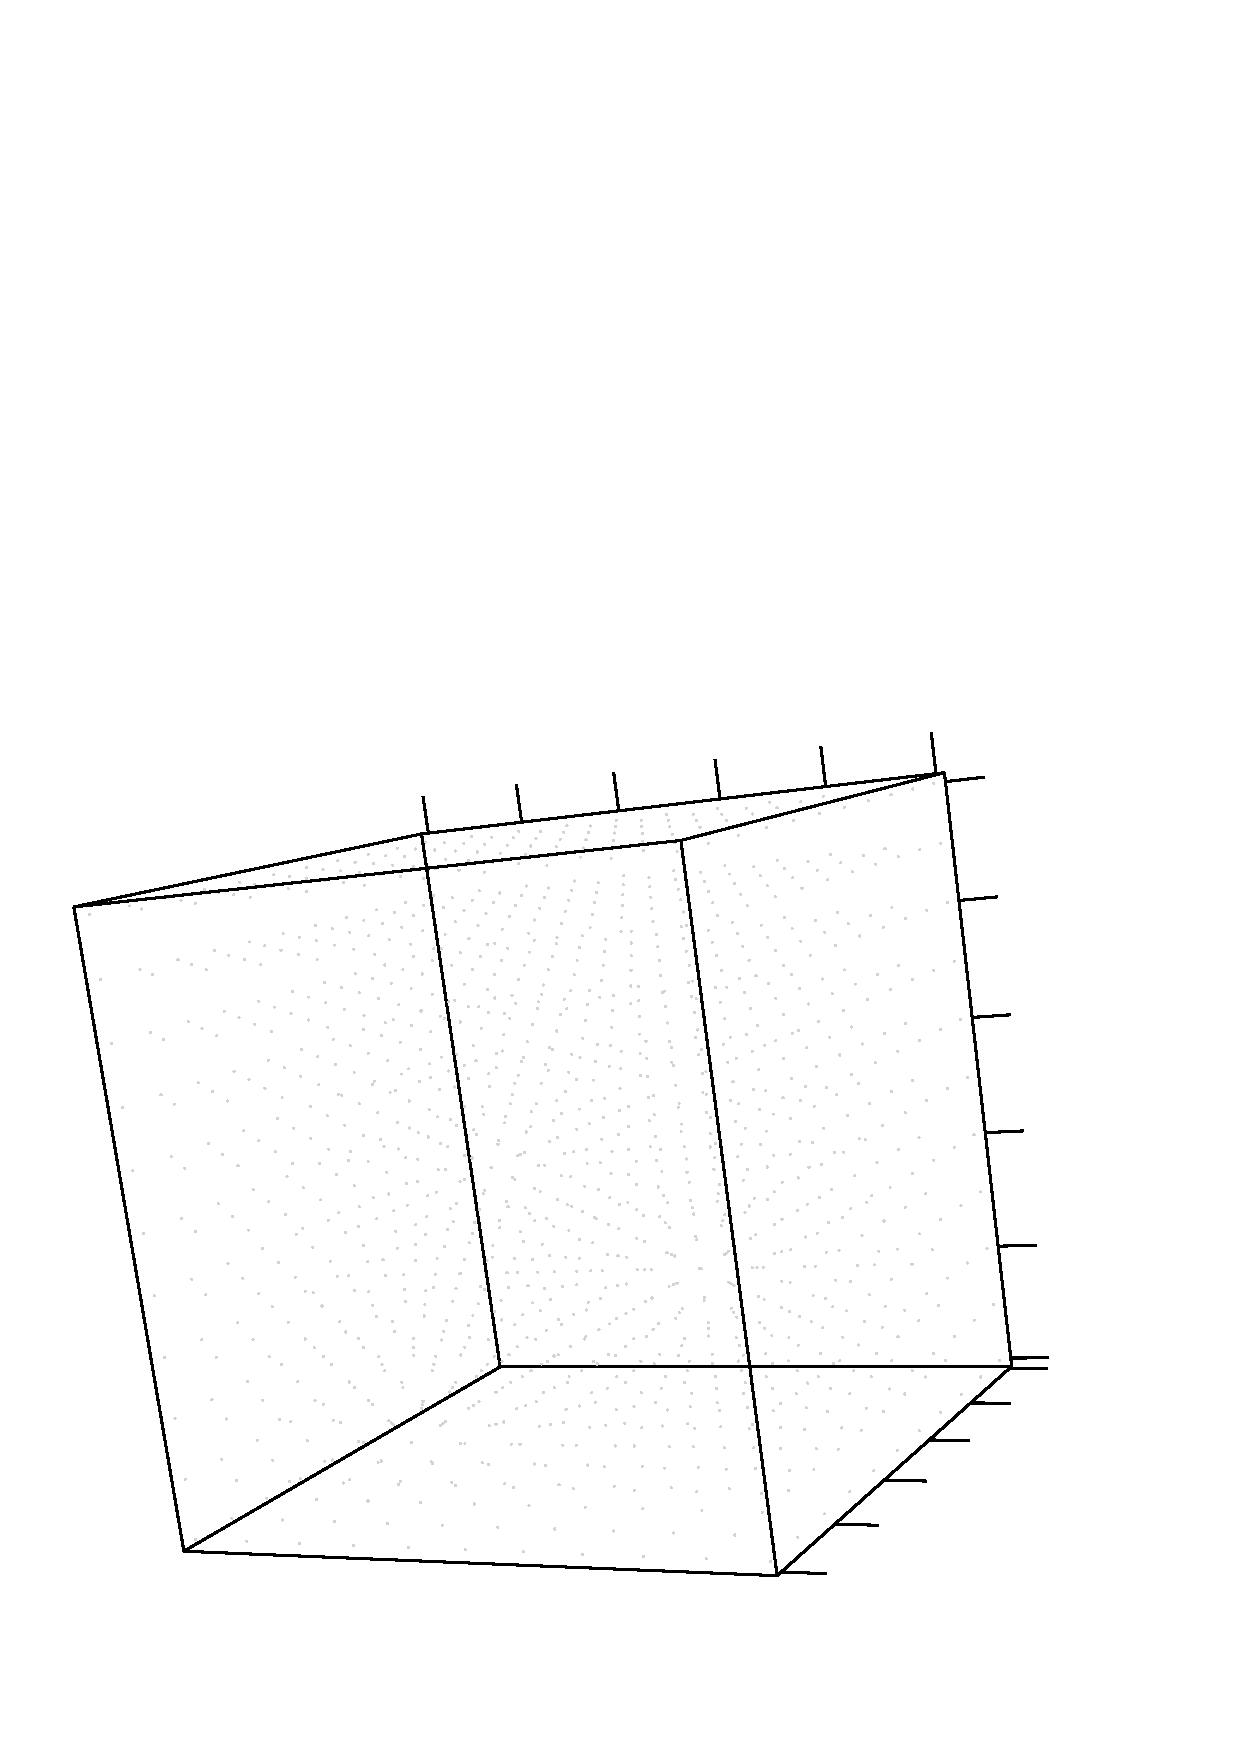
\includegraphics[width=.9\linewidth]{plot3d.pdf}
	\end{sidecaption}
\end{figure}

\begin{testiv}{Curse Dimensionality}{Exemple de Curse Dimensionality avec Simpop Local}

Le tableau ci-dessous présente le domaine de variations retenue par les experts pour les 5 paramètres du modèle agent Simpop Local, ainsi que le domaine de variation extrait de l'ensemble des meilleures valeurs de paramètres trouvées lors du calibrage \autocite{Schmitt2014, Schmitt2015}.

\begin{table}[H]
\centering
\begin{tabular}{@{}lll@{}}
\toprule
                   & Explored Domain & Solutions Domain          \\ \midrule
$P_{creation}$     & {[}0,1{]}       & ~{[} \SI{1.1e-06} ; \SI{1.3e-06} {]} \\
$P_{diffusion}$    & {[}0,1{]}       & ~{[} \SI{6.7e-07} ; \SI{6.9e-07} {]} \\
$InnovationImpact$ & {[}0,2{]}       & ~{[} \SI{7.7e-03} ; \SI{8.4e-03} {]} \\
$DistanceDecay$    & {[}0,4{]}       & ~{[} 0.66; 0.75 {]}       \\
$R_{max}$          & {[}1,40000{]}   & ~{[} 10090; 10465 {]}     \\
Volume             & 320000          & ~ \SI{4.7e-16}{}               \\ \bottomrule
\end{tabular}
%\caption{Valeur }
%\label{my-label}
\end{table}
Quelque soit finalement la résolution du plan d'expérience envisagé par l'utilisateur, celui-ci n'avait dans ce cas là que peu de chances de soulever l'existence d'une zone de solutions potentielles dans un espace de résolution aussi fin; seule l'usage d'une méta-heuristique pouvait détecter cette zone de validité du modèle, dans un volume qui représente au final $\SI{4.7e-16}{} / \num{320000} = \SI{1.5e-21}{} $ du volume total.

\end{testiv}


% Exemple pour illustrer ca au travers des problèmes SLocal qu'on a eu ?

% Jonction des trois fonctions objectifs

% Plutot une argumentation pour justifier de la nécessité d'explorer rapidement les modèles. Mais dans un deuxième temps, sur les analyses de sensibilités, car analyse de sensibilité c'est pas tip top

Contrairement à d'autres méthodes d'optimisations, les métaheuristiques font généralement appel à un processus d'échantillonnage (voir point \ref{enum_meta_b}) pour explorer de façon stochastique un espace de recherche de toute façon beaucoup trop vaste pour être parcouru de façon exhaustive. Cela permet de repousser en partie ce problème de couverture de l'espace de paramètres lié à l'augmentation de la dimensionnalité du problème, car nous verrons que les méta-heuristique opérant dans des espace de paramètres discrets mais aussi continus, sans qu'une discrétisation préalable soit nécessaire en amont.

C'est pour cela que \textcite[7]{Luke2013} nous propose de voir ce type de problème autrement, partant du postulat assez logique qu'une solution \enquote{même non optimale} est un point de départ pour l'amélioration de toute façon bien meilleure que \enquote{pas de solution du tout}.

\foreignblockquote{english}[{\cite[7]{Luke2013}}]{ Metaheuristics are applied to \enquote{I know it when I see it} problems. They're algorithms used to find answers to problems when you have very little to help you: you don't know what the optimal solution looks like, you don't know how to go about finding it in a principled way, you have very little heuristic information to go on, and brute-force search is out of the question because the space is too large. But if you're given a candidate solution to your problem, you can test it and assess how good it is. That is, you know a good one when you see it.}

Suivant ce raisonnement, la connaissance d'un problème se construit au travers d'une confrontation répétée de nos représentations, de nos interrogations avec la forme réelle et encore inconnue prise par celui-ci\Anote{paul_rationalite}. La carte de ce nouveau territoire se révélant peu à peu dans la projection sur l'espace des solutions des choix effectués lors de la sélection des nouveaux candidats à évaluer (solutions candidates).

Les métaheuristiques sont donc là pour faciliter l'exécution de cette tâche complexe et répétitive qui consisterait à améliorer notre connaissance du problème en proposant de façon pertinente de nouvelles solutions candidates à évaluer, ces dernières étant choisies si possible en fonction des résultats obtenus par les précédentes (voir point \ref{enum_meta_i}). La perspective d'une telle automatisation pose évidemment un certain nombre de questions.

Quels sont les choix mis à disposition de l'optimiseur pour améliorer la réponse attendue des solutions candidates entre chaque incrément ? \autocite[19]{Weise2011}

Une comparaison automatisée nécessite pour être mise en oeuvre de définir \begin{enumerate}[label=(\alph*)]
\item sur quelle base se fonde l'évaluation d'une solution,
\item la comparaison entre les solutions évaluées,
\item et la sélection de nouvelles solutions candidates.\end{enumerate}

Car l'optimiseur, tout comme nous, ne connaît pas directement la forme prise par l'espace des solutions, et doit bien concevoir en interne les choix permettant, par la sélection de nouvelles solutions candidates à évaluer, de progresser si possible vers une solution optimum.

De fait dans un tel scénario, et pour éviter une recherche aléatoire, l'évaluation de solution candidate renvoie à l'existence d'une expertise externe à l'optimiseur, le seul capable de formaliser ce qui différencie une bonne solution d'une mauvaise solution. On revient à parler ici d'heuristique, et de leurs diversités, car si celles-ci interviennent dans l'évaluation des solutions candidates (a), elles interviennent aussi dans les autres cas (b) et (c). Elles se présentent sous la forme de différents types de connaissances, interrogent différents espaces, et s'intègrent souvent sous la forme de composants dans la structure plastique des métaheuristiques.

L'injection de connaissances (voir point \ref{enum_meta_h} ) dans ce type d'algorithme métaheuristique est donc double, et opère à la fois de façon précise dans la formalisation d'un ou de plusieurs critères qui vont servir pour l'algorithme optimiseur à déterminer la qualité, bonne ou mauvaise, d'une solution candidate; et de l'autre elle intervient cette fois ci de façon moins contrôlable dans la façon dont l'expérimentateur va construire et paramétrer une métaheuristique pour l'adapter au mieux à son problème. La qualité interne (paramètre, structure) de la métaheuristique définit aussi en quelque sorte le processus d'exploration, ce qui explique aussi la dépendance de ce type d'algorithmes à l'environnement qu'ils doivent explorer.

\begin{figure}[!htb]
	\begin{sidecaption}[Projection de solutions candidates dans l'espace des objectifs]{Projection du vecteur de solution candidates $\{a \dotsc n\}$ dans l'espace des objectifs. Les flèches indiquent dans quel sens et sur quel plan se fait la projection des points. Les couleurs permettent de repérer quelle est la ligne de points que l'on a projetée, de la ligne 1 à 3 sur $(x,v)$ et de la ligne 1 à 4 sur $(y,v)$}[fig:spacePspaceOmultimodal]
	 \centering
	 	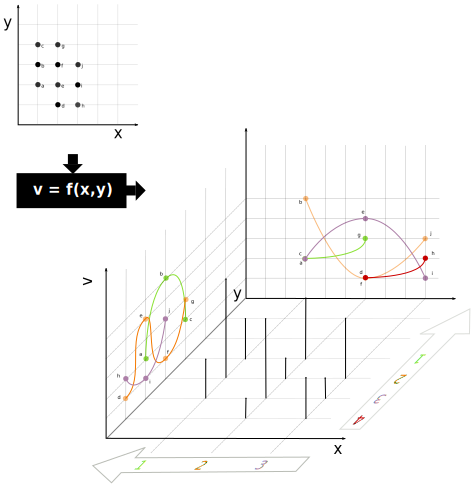
\includegraphics[width=.9\linewidth]{espaceP_espaceO_multimodal.pdf}
	\end{sidecaption}
\end{figure}

L'objectif est rendu complexe car la relation entretenue entre ces deux espaces, celui des solutions candidates disponibles, et celui des évaluations est bien souvent dissymétrique. Pour mieux comprendre cette relation, la figure \ref{fig:spacePspaceOmultimodal} illustre cette correspondance des solutions candidates $\{a \dotsc n\}$ décrites par leurs coordonnées $(x,y)$ lorsqu'elles sont projetées dans l'espace des objectifs $\mathbb{Y}$ en suivant la transformation attendue par la fonction boîte noire de dynamique non linéaire $f(x,y)$. Les valeurs $v = f(x,y)$ des différentes solutions candidates sont également projetées sur le plan 2D $(x,v)$ et $(y,v)$ pour mieux visualiser la forme prise par cette surface en 2D.

Pour visualiser la valeur $v$ prise par chacune des solutions candidates, on projette celle-ci dans l'espace $(x,y)$, ce qui nous permet de mieux constater l'éclatement des valeurs de $v$ sur la figure \ref{fig:xyspacePspaceOmultimodal}.

\begin{figure}[htbp]
	\begin{sidecaption}[Représentation des solutions candidates sur plusieurs plan vis-à-vis de la fitness]{Les couleurs indiquent la valeur $v = f(x,y)$ de chaque solution candidate $\{a \dotsc n\}$. $(v,x)$ et $(v,y)$ sont les plan extrait de la figure \ref{fig:spacePspaceOmultimodal}. On cherche ici à minimiser la valeur de $v$ :
\parbox{\marginparwidth}{
\begin{enumerate}[label={},labelindent=0pt,leftmargin=*]
        \item \sqbox{tangoBlue1} indique une fitness minimale, cf. qui maximise $v$
        \item \sqbox{tangoOrange1} indique une fitness intermédiaire et,
        \item \sqbox{tangoRed1} indique une fitness maximale, cf. qui minimise $v$
\end{enumerate}}}[fig:xyspacePspaceOmultimodal]
	 \centering
	  \subbottom[\label{subfig_xyespaceSolutionCandidate_a}]{
	 	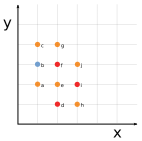
\includegraphics[width=0.4\linewidth]{xyespaceSolutionCandidate_a.pdf}
	 	}
	 \subbottom[\label{subfig_xyespaceSolutionCandidate_b}]{
	 	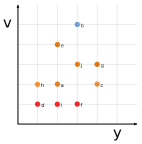
\includegraphics[width=.4\linewidth]{xyespaceSolutionCandidate_b.pdf}
	 	}
	 \subbottom[\label{subfig_xyespaceSolutionCandidate_c}]{
		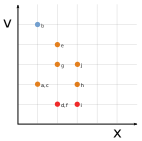
\includegraphics[width=.4\linewidth]{xyespaceSolutionCandidate_c.pdf}
		}
	\end{sidecaption}
\end{figure}


\begin{figure}[!htbp]
	\begin{sidecaption}[Déplacements simultanés dans l'espace des solutions candidates et dans l'espace des objectifs]{Représentation de deux déplacements dans l'espace des solutions candidates et son équivalent dans l'espace des objectifs
	\parbox{\marginparwidth}{
	\begin{enumerate}[label=(\alph*),labelindent=\parindent,leftmargin=*]
	        \item Partant de $b$, on se déplace d'une unité vers $c$ ou $a$, ce qui dans l'espace des objectifs équivaut également à un déplacement vers $h$; $v=2$ pour $v_h, v_a, v_c$
	        \item Partant de $b$, on se déplace toujours d'une unité vers $f$, ce qui dans l'espace des objectifs équivaut également à un déplacement vers $d$ et $i$; $v=1$ pour $v_d,v_i,v_f$
	\end{enumerate}}}[fig:xytrajectoire]
	 \centering
	  \subbottom[\label{subfig_xytrajectoire_a}]{
	 	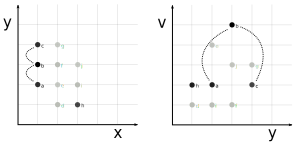
\includegraphics[width=0.8\linewidth]{xytrajectoire_a.pdf}
	 	}\qquad
	 \subbottom[\label{subfig_xytrajectoire_b}]{
	 	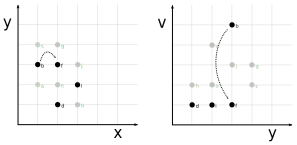
\includegraphics[width=.8\linewidth]{xytrajectoire_b.pdf}
	 	}
	\end{sidecaption}
\end{figure}

Deux solutions proches dans l'espace des solutions candidates peuvent amener à des résultats très différents, et inversement, pour deux évaluations proches peuvent correspondre des solutions candidates très éloignées, comme le détaille la figure \ref{fig:xytrajectoire}. Il s'agit d'une propriété bien connue des fonctions non linéaires, qu'elles soient décrites de façon explicite via le formalisme mathématique, ou de façon implicite dans l'expression des dynamiques complexes de modèles de simulation.

Il est clair que l'information récoltée par un tel déplacement basé sur une distance euclidienne dans le plan $(x,y)$ n'est pas pertinent dans la recherche des emplacements possibles des meilleures solutions (voir figure \ref{fig:xytrajectoire}). Il semble par exemple plus intéressant pour l'optimiseur d'accéder aux solutions par le prisme d'ensembles construits sur la base d'une valeur $v$ commune (voir figure \ref{fig:xyspacePspaceOmultimodal}). Une information qui peut être exploitée de multiples façons, toujours en permettant à l'optimiseur de déterminer un nouvel ensemble de solutions candidates à évaluer.

Si l'obtention d'une cartographie complète d'un tel espace de solutions peut être l'objectif de ce type de raisonnement, la recherche d'un optimum en est un autre. Dans un cas on aura tendance à maximiser la diversité dans le choix de solutions candidates à évaluer, afin d'essayer de couvrir au mieux le territoire à explorer. Cette idée on la retrouve dans l'établissement d'une \textit{fitness landscape}, ou dans sa version multi-objectif, d'un \textit{problem landscape} \autocite[93-94]{Weise2011}, un paysage cumulé de l'espace des objectifs indiquant toutes les valeurs prises par ceux-ci au cours de l'exploration\Anote{paysage_cumule}. Un espace mis à profit par l'optimiseur pour améliorer la proposition de solution candidate, par exemple en se basant sur la construction de cluster de valeurs intéressantes comme indiqué précédemment, ou encore en cherchant à favoriser les zones de cet espace encore peu explorées, etc. Alors que dans le cas d'une optimisation pour la calibration ou la prédiction, trouver le plus rapidement possible un minimum local ou global peut constituer un objectif suffisant.

En réalité, ces deux objectifs sont souvent liés, et c'est souvent l'expertise humaine intervenant de façon externe à l'optimiseur qui va déterminer l'importance de l'un ou de l'autre dans la stratégie à suivre. Dans le cas par exemple d'une optimisation de paramètres nécessaire à la marche efficiente d'une centrale nucléaire, la découverte d'un minimum local robuste peut s'avérer beaucoup plus intéressante qu'un minimum global instable. La topologie proche de l'espace des solutions déjà exploré peut constituer un facteur de connaissance d'intervention plus ou moins importante dans l'expertise d'une bonne ou d'une mauvaise solution.

Cette mécanique on la retrouve également à un autre niveau, dans le fonctionnement interne des métaheuristiques. En effet, celles-ci s'appuient le plus souvent sur la métaphore biologique évolutive pour mettre en tension une recherche de solutions guidée toute à la fois par l'\textit{exploration} (trouver des solutions originales), et l'\textit{exploitation} (améliorer les solutions existantes).

\begin{figure}[!htbp]
\begin{sidecaption}[Recherche d'un minimum global]{Recherche d'un minimum global.}[fig:hmap2ab]
 \centering
 \subbottom[Une fonction $f(x)$ présentant un unique minimum global.\label{subfig_hmap2ab_a}]{
 	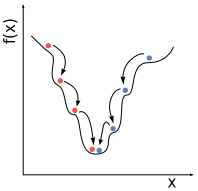
\includegraphics[width=.4\linewidth]{heightmap2a.pdf}
 	}\qquad
 \subbottom[Une fonction $f(x)$ présentant un minimum local et global.\label{subfig_hmap2ab_b}]{
	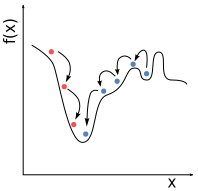
\includegraphics[width=.4\linewidth]{heightmap2b.pdf}
	}
\end{sidecaption}
\end{figure}

Les opérateurs intervenant comme stratégies dans la médiation de ces deux concepts sont conçus pour éviter à l'optimiseur un certain nombre d'écueils. Trop longue pour être abordée ici de façon exhaustive, cette liste évoquant les problèmes et solutions qui résultent du rapport entre les formes de problèmes abordés et les faiblesses génériques ou dépendantes des métaheuristiques utilisées, \textcite{Weise2011} en donne une description experte sur une centaine de pages. On peut également se référer à une autre synthèse, abordant ces problèmes avec un angle un peu plus spécifique aux algorithmes évolutionnaires, réalisée en 2001 par \textcite[316-445]{Deb2001}.

En se limitant aux pièges dépendant de la topologie de l'espace des solutions (voir point \ref{enum_meta_e}), \textcite[140]{Weise2011} a proposé un tableau synthétique dont on extrait ici quelques exemples légèrement modifiés pour éclairer notre argumentaire. Les exemples des figures \ref{fig:hmap2ab} et \ref{fig:hmap2cd} mettent en oeuvre un optimiseur générant de façon incrémentale de nouvelles solutions, chacune représentée par un point. Il faut donc lire ces exemples en tenant compte du fait qu'ils présentent une représentation cumulative des différents points parcourus dans le temps par l'optimiseur.

La figure \ref{fig:hmap2ab} démontre un fonctionnement normal de l'optimiseur, capable quelque soit son placement initial (rouge ou bleu), de trouver le minimum global d'une fonction relativement simple \ref{subfig_hmap2ab_a}. Un comportement équivalent est observable dans la figure \ref{subfig_hmap2ab_b}, le compromis \enquote{exploitation - exploration} étant suffisant pour que l'optimiseur bleu surmonte l'obstacle posé par la présence d'un minimum local dans cette fonction.

\begin{figure}[!htbp]
  \begin{sidecaption}[Des fonctions difficiles à optimiser du fait de paysages complexes]{Deux types de fonctions sont rendues difficiles à optimiser du fait d'une topologie marquée.}[fig:hmap2cd]
  \centering
  \subbottom[Une fonction $f(x)$ multimodale acceptant plusieurs minimum locaux, et un seul minimum global.\label{subfig_hmap2cd_c}]{
  	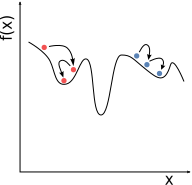
\includegraphics[width=.4\linewidth]{heightmap2e.pdf}
  	}\qquad
  \subbottom[Une fonction $f(x)$ contenant très peu d'information de gradient pour guider l'optimiseur.\label{subfig_hmap2cd_d}]{
	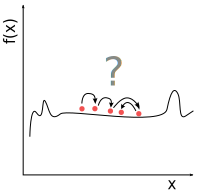
\includegraphics[width=.4\linewidth]{heightmap2c.pdf}
  	}
 \end{sidecaption}
\end{figure}

A l'inverse, on perçoit bien sur ce schéma \ref{subfig_hmap2cd_c} quel effet peut avoir un déséquilibre entre les deux stratégies, une exploitation trop appuyée au détriment de l'exploration amenant souvent à une convergence\Anote{def_convergence} prématurée, c'est-à-dire à un piège dans un optimum local.

La figure \ref{subfig_hmap2cd_d} montre également que face à une topologie de fonction présentant un plateau relativement uniforme, l'optimiseur sera en peine pour trouver un minimum, même local. Un paramétrage différent de l'exploration pourra peut être résoudre ce problème, sans pour autant que l'on en soit sur.

Ce qui nous permet d'évoquer une faiblesse connue des métaheuristiques, héritée des remarques déjà faites sur les algorithmes d'optimisations stochastique\Anote{stochastic_note} dans laquelle on les place habituellement. La découverte garantie d'une solution globale optimale est en général difficile avec ce type d'algorithmes (voir point \ref{enum_meta_d})\Anote{equipe_mixite}, au moins pour deux raisons :

\begin{enumerate}
\item la variabilité qui opère lors de la sélection des solutions candidates à un instant $t$ ne permet pas de garantir qu'il n'existe pas quelque part une solution candidate sélectionée à $t+1$ dont l'évaluation révélera un meilleur optimum. La définition d'un critère d'arrêt est donc rendue délicate.
\item La variabilité dans l'établissement d'une trajectoire de recherche implique qu'un algorithme de même qualité puisse passer une première fois à côté d'un optimum, et une deuxième fois trouver celui-ci.
\end{enumerate}

\begin{figure}[!htbp]
\begin{sidecaption}[Représentation de la navigation indirecte d'une métaheuristique dans un espace de solution]{Représentation d'une navigation indirecte de l'optimiseur dans un espace de solution $z = f(x,y)$.}[fig:hmap1]
  \centering
  \subbottom[\label{subfig_hmap_a}]{
  	\includegraphics[width=.4\linewidth]{heightmap1a.png}
  	}\qquad
  \subbottom[\label{subfig_hmap_b}]{
	\includegraphics[width=.4\linewidth]{heightmap1b.png}
  	}
\end{sidecaption}
\end{figure}

Pour mieux comprendre les problèmes posés par des espaces de solutions multi-modaux, déjà figurés en deux dimensions dans \ref{subfig_hmap2cd_c}, on représente cette fois ci dans la figure \ref{fig:hmap1} l'optimiseur dans un espace en trois dimensions similaire à celui vu dans la figure \ref{fig:spacePspaceOmultimodal}, à la recherche d'un optimum global. La fonction ainsi représentée comporte deux entrées $(x,y)$, et une sortie $z = f(x,y)$ représentant la valeur numérique résultat de l'optimisation.

Attention à la lecture de ces schémas, il ne faut pas oublier que l'optimiseur \textbf{ne se déplace pas directement} sur le terrain visible dans la figure \ref{subfig_hmap_a}, et pour laquelle celui-ci n'a justement aucune visibilité. C'est un peu comme visualiser un labyrinthe de l'extérieur sur une feuille, puis de l'intérieur quand on s'y projette, la difficulté pour résoudre celui-ci n'est plus la même. La visibilité dont dispose l'optimiseur est celle des résultats de solutions candidates déjà évaluées (voir point \ref{enum_meta_i}). Il s'agit donc de proposer de nouvelles solutions candidates soit en les composant à partir d'une manipulation des solutions candidates déjà évaluées, soit en introduisant de toutes nouvelles solutions candidates prises de façon aléatoire. Au cours de l'itération mesurant la progression de l'algorithme, c'est bien l'évaluation de cette nouvelle population de solutions candidates qui détermine s'il y a effectivement eu un déplacement qualitatif dans l'espace des solutions evaluées. Le déplacement du point rouge dans cet espace n'est donc effectif que si on trouve à un instant $t + 1$ une solution plus intéressante qu'à l'instant $t$.

A partir des résultats de la première solution candidate évaluée figurée ici en rouge dans \ref{fig:hmap1}, les opérateurs de recherches soumis à l'aléa d'une recomposition ou d'un tirage aléatoire peuvent tout à fait proposer un candidat à $(x,y)_{t+1}$ qui débouche sur un résultat $z = f(x,y)$ plaçant l'optimiseur dans le sillon d'un gradient de pente parmi plusieurs. Ce qui mènera probablement l'optimiseur à découvrir des optimums de qualités très différentes : $A$ (local), $B$ (global), $C$ (local), $D$ (local).

Autrement dit, en plus de la stochasticité inhérente de ces algorithmes, non seulement un algorithme de type $A$ n'aura pas les mêmes résultats qu'un algorithme de type $B$, mais celui-ci sera également différent d'un algorithme $A'$ du fait d'un paramétrage différent.

Comme déjà évoqué dans les différentes définitions, on retrouve ici la qualité de flexibilité des métaheuristiques, permettant de transformer ce qui pourrait de prime abord paraître pour un défaut, en qualité. L'utilisation de celle-ci permettant d'étendre toujours un peu plus leurs champs d'utilisation, en facilitant la réponse aux questions suivantes\Anote{q_ppr} :
\begin{enumerate}
\item  \foreignquote{english}{What parameter settings do I use to get good results when applying heuristic method X to problem Y?}
\item  \foreignquote{english}{How do I adjust the parameters of heuristic X so I get better results on problem Y?}
\item \foreignquote{english}{Which is \enquote{better}, heuristic X or heuristic Y?}
\end{enumerate}

On pourrait ainsi ne retenir que cette citation de source inconnue, lorsqu'elle définit une métaheuristique comme \foreignquote{english}{ a pretty good rule for finding pretty good rules.}

Cette flexibilité vient compléter et compenser efficacement cet horizon de connaissance assez limité, nécessaire à une généricité d'emploi. Les métaheuristiques fournissent ainsi le support générique initial pour en faire un outil d'usage indépendant du problème, tout en fournissant les outils pour favoriser également leur propre modification en vue d'une amélioration de résultat pour un problème donné. Elles cumulent donc ces deux propriétés de dépendance et d'indépendance face à un problème donné.

De plus, la recherche dans cette discipline ne se contente pas d'organiser une forme de compétition qui mènerait à elle seule, par l'apprentissage répété de fonctions aussi standardisées que celles utilisées dans les figures précédentes, à une surestimation de certains algorithmes\Anote{test_fonction_surutilisation}, et se nourrit également d'une recherche plus appliquée à des problématiques réelles. Ce qui permet par effet retour, d'espérer voir appliquer à des formes de problèmes génériques, des opérateurs dédiés à l'origine à des problématiques spécifiques. La construction et l'évaluation d'heuristiques plus performantes servant indirectement une cause plus générale.

Enfin, une des propriétés qui n'a pas encore été introduite dans ce résumé est la capacité de notation et de description abstraite des métaheuristiques (voir point \ref{enum_meta_f} ). Des concepts de plus haut niveau sont introduits pour désigner l'expression et la manipulation d'heuristiques et de classes d'heuristiques dans un système composant la métaheuristique. Mais avant de pouvoir introduire ces subtilités de typologie propre à chaque classe de métaheuristique, il faut également rappeler l'existence d'une base commune de formalisation mathématique permettant la description des problèmes. Autrement dit, cela revient à introduire ou à poser sur une partie des mots déjà utilisés dans cette section, un certain nombre de notations mathématiques d'utilisation relativement standard dans cette communauté informatique utilisant les métaheuristiques.

Il nous restera également à aborder dans la section suivante, la question des \textbf{moyens} mis à disposition de l'optimiseur pour opérer la sélection de nouveaux candidats à évaluer. Jusqu'ici seule une représentation de ces solutions candidates dans l'espace des solutions candidates possibles a été abordée, ainsi que l'espace contenant les résultats des solutions candidates évaluées. Mais ces deux espaces ne constituent pas les véritables espaces sur lesquels l'optimiseur est amené à travailler, et cela bien qu'il puisse les intégrer à son expertise pour séléctionner de nouveaux candidats à l'évaluation\Anote{remarque_section_metaheuristique}.

L'introduction d'un nouvel \enquote{espace de recherche} est nécessaire, et  correspond à la somme des entrées, des paramètres, sur lequel l'optimiseur va pouvoir jouer directement, afin de modifier cette fois-ci indirectement l'expression de la solution candidate ensuite évaluée.

Autrement dit, il faut retenir qu'une solution candidate fait partie d'un espace de solutions candidates possibles, et que l'exploration de ce dernier est dépendante des bornes fixées par l'expert pour délimiter l'espace de recherche de chacun des entrants. L'objectif étant notamment de limiter le champ de recherche de l'optimiseur à des valeurs empiriquement et théoriquement possibles. Ce qui introduit aussi la possibilité d'un nouveau \textit{mapping} entre les valeurs de ces deux espaces, de recherche et du phénomène à évaluer, qui ne sont pas nécessairement de même nature.

On peut s'appuyer sur l'exemple de bras robotisé donné par \autocite{Weise2011} pour illustrer ce cas. On a d'un côté des bornes de paramètres délimitant le positionnement des différents éléments de bras d'un robot, limité par sa structure, et de l'autre l'expression spatiale qu'il est possible d'exprimer par une combinaison unique de valeurs de paramètres. L'optimiseur s'appuie sur l'évaluation de cette configuration spatiale à l'aide des critères qu'on lui a donnés pour induire des opérations non pas dans l'espace d'expression spatialisée du bras, dont on n'a pas la maitrise directe, mais dans la modification des valeurs de paramètres susceptible d'améliorer ce résultat.

\subsubsection{Une formulation mathématique standardisée pour encadrer les problèmes d'optimisation et les métaheuristiques}
\label{sssec:math_opti}

%search space p 82
%structure p 101
% pareto ranking p 275

Pour comprendre comment se déroule de façon générale la résolution d'un problème d'optimisation, il faut poser un certain nombre de notions qui nous seront utiles par la suite. Cet exercice de description plus mathématique et générique s'appuie là encore principalement sur les écrits de \textcite{Weise2011}

La première étape selon Weise dans la construction d'un problème d'optimisation est de définir le type de structure qui peut être associée à l'expression des solutions possibles et spécifiques à notre problème.

Autrement dit, il s'agit de déterminer quel est l'espace dans lequel évolue la donnée figurant la solution attendue pour cette optimisation. L'expression de cette solution peut appartenir à l'espace des réels $\mathbb{R}$, comme par exemple une valeur numérique se rapportant à l'optimisation d'une fonction mathématique. Mais celle-ci peut également s'exprimer dans un repère beaucoup plus complexe, en faisant référence par exemple à un repère géométrique définissant le cadre  d'une forme à optimiser comme une pièce de moteur, une pièce d'avion, etc. \autocite[43]{Weise2011}
\medskip

Cet espace du problème (\textit{problem space}) $\mathbb{X}$ est défini comme \foreignquote{english}{ [...] the set containing all elements $x$ which could be its solution.}

\medskip

Une solution candidate $x$ est quant à elle définie comme \foreignquote{english}{ [...] an element of the problem space $ \mathbb{X}$ of a certain optimization problem.}

\medskip

L'objectif de l'optimisation est donc de trouver par le biais d'un algorithme adapté l'ensemble des solutions candidates $x^*$ appartenant à l'espace du problème répondant le mieux aux critères définis par l'utilisateur. Ce qui suppose de pouvoir qualifier une solution candidate $x_1$ tiré de $\mathbb{X}$ par rapport à une autre solution candidate $x_2$ elle aussi tiré de $\mathbb{X}$.

\medskip

\textit{Une deuxième étape logique serait donc d'établir comment se fait la mesure établissant la qualité d'une solution ?}

\medskip

Comme défini précédemment, ce qui va guider l'algorithme optimiseur dans sa prise de décision, c'est l'évaluation d'une fonction heuristique, ou d'une fonction objectif (\textit{objective function})\Anote{difference_objective_heuristique}

\medskip

\foreignblockquote{english}{An objective function $f: \mathbb{X} \to \mathbb{R}$ is a mathematical function which is subject to optimization.}

\medskip

Cette fonction objectif lorsqu'elle prend pour paramètre un élément candidat $x$ pris dans l'espace du problème $ \mathbb{X}$ renvoie une valeur définissant sa qualité par rapport au problème posé. \autocite[44]{Weise2011}

\sloppy La plupart des problèmes nécessitent toutefois d'optimiser plusieurs critères simultanément. La relation entre ces critères peut d'ailleurs être elle aussi multiple : dépendante (conflictuelle, en harmonie), indépendante. Nous allons donc nous intéresser directement à la définition de ce type de problème, résumable ainsi :  $min(f_1(x), \dotsc, f_k(x)$ avec $k > 2$

La littérature fait également plus souvent référence à ce type de problème en faisant appel à une notation sous forme de fonction vecteurs. Un ensemble $\vec{f} : \mathbb{X} \to \mathbb{R}^n$ fait de $n$ fonction objectif $f_i : \mathbb{X} \to \mathbb{R}$ avec $\forall i \in 1 \dotsc n$. Appliquée à une solution candidate $x \in \mathbb{X}$ cette fonction renvoie un vecteur de réel de dimension $n$ qui peuvent être projeté dans un espace $\mathbb{R}^n$, aussi appelé espace des objectifs (\textit{objective space}) $\mathbb{Y}$.

En résumé, à chaque association d'un vecteur de fonction objectif $\vec{f}$ et d'une solution candidate $x$ correspond après évaluation un vecteur de réel de dimension $n$ permettant le positionnement de la solution candidate dans l'espace $\mathbb{R}^n$ des objectifs aussi nommé $\mathbb{Y}$.

C'est à partir du positionnement des solutions candidates dans cet espace $\mathbb{Y}$ que l'optimiseur va décider de la prochaine solution candidate à évaluer.
\medskip

\textit{Dès lors, comment ce choix se fait-il dans une perspective multi-objectifs a priori contradictoires ?}

\begin{figure}[!hbtp]
	\begin{sidecaption}[Représentation de la fonction mathématique de Schaffer]{ Pour la valeur $x = 0$, $f1(x) = 0 $ et $f2(x) = 4 $, pour $x = 2$,  $f1(x) = 4 $ et $f2(x) = 0 $ , donc la configuration inverse. La solution pour minimiser les deux fonctions $f1$ et $f2$ tient donc forcément dans un compromis dans la valeur prise par $x$.}[fig:S_Schaffer]
	\centering
	\begin{tikzpicture}[line cap=round,line join=round,>=triangle 45,x=1.0cm,y=1.0cm]
	\draw [color=cqcqcq,dash pattern=on 1pt off 1pt, xstep=1.0cm,ystep=1.0cm] (-5,-1) grid (5,5);
	\draw[->,color=black] (-5,0) -- (5,0);
	\foreach \x in {-5,-4,-3,-2,-1,1,2,3,4}
	\draw[shift={(\x,0)},color=black] (0pt,2pt) -- (0pt,-2pt) node[below] {\footnotesize $\x$};
	\draw[->,color=black] (0,-1) -- (0,5);
	\foreach \y in {-1,1,2,3,4}
	\draw[shift={(0,\y)},color=black] (2pt,0pt) -- (-2pt,0pt) node[left] {\footnotesize $\y$};
	\draw[color=black] (0pt,-10pt) node[right] {\footnotesize $0$};
	\clip(-5,-1) rectangle (5,5);
	\draw[color=ttttff] plot[raw gnuplot, id=func2] function{set samples 100; set xrange [-4.9:4.9]; plot x**2};
	\draw[color=fftttt] plot[raw gnuplot, id=func3] function{set samples 100; set xrange [-4.9:4.9]; plot (x-2)**2};
	\begin{scriptsize}
	\draw[color=ttttff] (-2.26,6.14) node {$f$};
	\draw[color=fftttt] (-0.24,6.14) node {$g$};
	\end{scriptsize}
	\end{tikzpicture}
 \end{sidecaption}
\end{figure}

%\sloppy

\pagebreak

Si on prend pour exemple la fonction multi-objectifs de Schaeffer décrite dans l'équation \ref{eq:schaffer}, $f1(x)$ and $f2(x)$ deux fonctions objectifs à minimiser $\vec{f} = (f1(x),f2(x))^T$  avec $\vec{f}: \mathbb{X} \to \mathbb{R}^2$

\begin{equation} \label{eq:schaffer}
Minimize =
	\begin{cases}
	 f1(x) = x^2 \\
	 f2(x) = (x-2)^2
	\end{cases}
\end{equation}

Si on superpose les deux fonctions comme dans la figure \ref{fig:S_Schaffer}, on voit bien qu'elles sont contradictoires, il s'agit donc de trouver un compromis.

Cette opération que nous pratiquons tous les jours sans forcément le savoir peut être plus facilement expliquée en faisant appel à cet exemple concret. Dans le cas d'un acheteur à la recherche d'une voiture à la fois économe de par sa faible consommation et si possible disponible à un moindre coût, celui-ci devra bien se plier à l'exercice de positionnement des voitures résumé dans le graphique \ref{fig:voiture}.

Dans le graphique \ref{subfig_voiture:b} on constate rapidement que le modèle de voiture que le client est susceptible d'acheter a de fortes chances de se trouver dans la liste de voitures $\{ A,B,C,D,E \}$ colorées en rouge, aussi appelée \enquote{front de Pareto}, ou \enquote{optimum de Pareto}. Ce terme apparaît en économie en 1950, en référence directe des travaux de l'économiste italien Vilfredo Pareto. Le lecteur plus curieux de ces questions pourra trouver de multiples points d'entrées sur ces questions dans les publications suivantes \autocites{Ehrgott2012, Koksalan2011, Koksalan2013}.

%\pagebreak
\bigskip

\begin{testiv}{Définir des objectifs pour le modèle Ants}{Définir des objectifs pour le modèle Ants}

Pour le modèle \textbf{Ants}, on a vu qu'il existait trois paramètres pouvant être amenés à varier en entrée du modèle.

Les paramètres d'évaporation $Evaporation-rate$ et $Diffusion-rate$ varie chacun dans le domaine $\mathbb{R}$, entre les valeurs $0.0$ et $99.0$ auquel on associe maintenant trois fonctions objectifs.

Le paramètre de population est réglé par défaut à $125$ fourmis dans la colonie, mais il est également possible de le faire varier sur $\mathbb{N}$ entre $0$ et $250$.

\begin{itemize}[noitemsep,nolistsep]
\item L'espace $\mathbb{X}$ est un cube $\{\mathbb{N},\mathbb{R},\mathbb{R}\}$ de bornes $\{[0,250], [0,99.0], [0,99.0]\}$
\item L'espace $\mathbb{Y}$ associe pour un point $x \in \mathbb{X}$ un point de valeur ${f_1,f_2,f_3}$ dans le domaine non borné $\{\mathbb{R},\mathbb{R},\mathbb{R}\}$
\end{itemize}

Les fonctions objectifs $\{f_1,f_2,f_3\}$  se base chacune sur le temps écoulé entre le début de la simulation $t_0$ et le temps indiqué pour la disparition complète d'un tas de nourriture.

\begin{enumerate}[noitemsep,nolistsep]
\item $f_1$ stocke le pas de temps de simulation (\textit{ticks}) à laquel le tas de nourriture 1 disparaît.
\item $f_2$ stocke le pas de temps de simulation (\textit{ticks}) à laquel le tas de nourriture 2 disparaît.
\item $f_3$ stocke le pas de temps de simulation (\textit{ticks}) à laquel le tas de nourriture 3 disparaît.
\end{enumerate}

Pour pouvoir rapporter ces valeurs à l'optimiseur, encore faut-il que cette simulation se finisse d'une façon ou d'une autre. Il faut donc fixer \textbf{une condition d'arrêt} pour remplacer le clic sur le bouton stop effectué par l'utilisateur dans Netlogo. La condition d'arrêt la plus simple ici est de stopper la simulation lorsque il n'y a plus aucune nourriture disponible.

Attention toutefois, il faut savoir que l'optimiseur, dans ses multiples tentatives pour trouver le meilleur jeu de valeurs de paramètres qui mimise les trois fonctions objectifs, risque de produire des combinaisons qui peuvent mettre le modèle ou les hypothèses du modèle en difficulté. \textit{Effectivement que se passe-t-il dans notre modèle de simulation si les valeurs de paramètres sont les suivants ? }

\begin{table}[H]
\centering
\caption{Testons ces conditions avec une même graine aléatoire (42)}
\label{tab:experience}
\begin{tabular}{lllll}
\hline
  & $Population$ & $Evaporation-Rate$ & $Diffusion-Rate$ & $t_{stop}$ \\ \hline
1 & 125        & 25.0             & 25.0  & 1554 \textit{ticks} \\
2 & 0          & 25.0             & 25.0  & $\infty$ \\
3 & 25         & 25.0             & 25.0  & 8825 \textit{ticks} \\
4 & 125        & 0.0              & 0.0   & 1374 \textit{ticks} \\
5 & 125        & 99.0             & 0.0   & 1261 \textit{ticks} \\
6 & 125        & 0.0              & 99.0  & 1201 \textit{ticks} \\
7 & 125        & 99.0             & 99.0  & 1254 \textit{ticks} \\ \hline
\end{tabular}
\end{table}

Dans le cas (2) la simulation ne s'arrête jamais, car la condition d'arrêt n'est jamais remplie. Ce comportement n'est clairement pas intéressant et risque tout simplement de bloquer l'exploration réalisée par la métaheuristique, il faut donc fixer une valeur $> 0$ pour la population de fourmis.

Le cas (3) montre qu'avec moins de fourmis, il faut beaucoup plus de temps à la simulation pour que la condition d'arrêt soit remplie. Il peut donc y'avoir une très forte variabilité dans les durées d'exécution du modèle en fonction des valeurs de paramètres sélectionnés pour évaluation.

Les cas (4,5,6) sont intéressants, car ils sont susceptibles de produire des résultats contre-intuitifs. En effet, en terme de durée d'exécution totale, on obtient pour cette graine aléatoire de meilleurs résultats qu'avec des valeurs de paramètres pris au hasard (1). Un mauvais paramétrage produit un effet d'aspiration qui fait que des fourmis se dirigeant potentiellement vers le tas de nourriture sont détournées de leurs traces par cette piste olfactive.

\begin{figure}[H]
	 \centering
	 	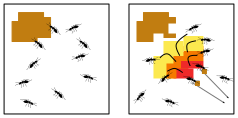
\includegraphics[width=.7\linewidth]{ant.pdf}
\end{figure}

Cela peut également s'expliquer par le débordement et la mise en défaut des mécanismes prévus initialement par le modélisateur, car les fourmis ne captent les traces chimiques qu'entre $0.05$ et $2$. Or la diffusion ou l'évaporation se cumule en partant d'une valeur unitaire à $60$, qui est l'équivalent de la trace chimique déposée sur chaque \textit{patch} pour une fourmi ayant trouvé de la nourriture. Donc dans tous ces cas là, les mécanismes du modèle sont quasi-innefficaces, et se rapportent au cas (3) qui met en jeu une simple marche aléatoire des fourmis.

\textit{L'optimiseur sera-t-il capable de trouver de meilleures valeurs dans cette zone d'activation ?} Si ce n'est pas le cas, il faudra revoir les paramètres ou le fonctionnement de notre mécanisme guidant le comportement de dépôt et de détection de traces associé à chaque fourmi.

Plusieurs pistes peuvent être indiquées au modélisateur pour éviter ou limiter l'apparition de comportement pouvant bloquer l'exploration :

\begin{itemize}[noitemsep,nolistsep]
	\item fixer les valeurs de paramètres pouvant poser problème, quitte à les faire varier par la suite.
	\item identifier en amont les combinaisons de jeu de valeurs de paramètres susceptibles de poser problème, pour ensuite les interdire à l'optimiseur.
	\item introduire un paramètre ou un mécanisme artefact (c'est-à-dire qui est extérieur aux hypothèses originales) dans le modèle, par exemple en fixant un seuil maximum d'objets (tortues dans Netlogo).
	\item introduire des critères d'arrêts plus restrictifs.
	\item pénaliser les comportements posant problème directement dans les fonctions objectifs.
\end{itemize}

Un autre type d'erreur peut encore intervenir lors de telles explorations, l'exploration intensive de l'espace de recherche combiné des différents paramètres et le grand nombre d'exécutions des simulations mettent à rude épreuve le déroulement des programmes, ce qui permet de faire remonter un certain nombre d'erreurs (division par zéro, comportements inattendus, dépassement mémoire, etc.) En ce sens, ce type d'exploration participe de la validation interne du modèle.

\end{testiv}


\begin{figure}[htbp]
	\begin{sidecaption}[Exemple de front de Pareto sur des voitures]{Exemple simplifié d'une catégorisation de voitures selon deux axes comprenant d'une part le coût d'achat et d'autre part la consommation de chaque voiture.}[fig:voiture]
	\centering
	  \subtop[\label{subfig_voiture:a}]{
  	\includegraphics[width=.4\linewidth]{opti1.png}
  	}\qquad
    \subtop[\label{subfig_voiture:b}]{
	\includegraphics[width=.4\linewidth]{opti2.png}
  	}
    \subtop[\label{subfig_voiture:c}]{
  	\includegraphics[width=.4\linewidth]{opti3.png}
  	}
 \end{sidecaption}
\end{figure}

\sloppy En regardant en détail les capacités des voitures figurant dans ce front \ref{subfig_voiture:c}, on voit bien que chacune d'entre elle domine une partie des autres voitures sur au moins un des deux objectifs. Si on prend le cas de la voiture F, celle-ci n'est pas prise en compte dans les solutions optimums, car le point est dominé sur ses deux objectifs par d'autres voitures : $ prix(B) < prix(F) < prix(A) $ et $consommation(A) < consommation (B) < consommation(F)$.

Le front de Pareto renvoie un ensemble de solutions compromis optimal, l'expertise finale sur la ou les solutions à adopter est donc le résultat d'un choix expert externe introduit comme support à l'algorithme optimiseur. Dans notre exemple, l'acheteur devra pour finaliser son achat mettre en avant au moins un des deux critères afin de départager les voitures.

Si certains algorithmes ont introduit cette expertise par le biais d'une sélection interactive guidant l'optimiseur à chaque étape de sa recherche, ce n'est pas cet usage qui nous intéresse ici. L'expertise n'intervient qu'une fois l'ensemble des solutions sélectionnées par l'optimiseur stabilisés, dans l'observation experte des résultats finaux.

Dans notre cas, on considère que l'optimiseur doit sélectionner avec les moyens qu'on lui a fournis les solutions candidates sur lesquels il doit miser pour converger. Il doit donc être capable de séparer les solutions en appliquant un ou plusieurs critères de séparation. Il existe plusieurs types de stratégies (\textit{Agreggation based, Criterion based, Dominance based, Indicator based}), et chacune d'elle peut être croisée ou dérivée en de multiples variantes \autocites[28]{Zitzler1999a, Deb2001}[7]{Liefooghe2009}. Nous limiterons ici notre analyse à un seul de ces cas, en nous focalisant d'ores et déjà sur les méthodes les plus utilisées en EC, basées sur la dominance celles-ci sont directement inspirées des travaux de Pareto.

% TODO : Finir ce paragraphe historique rapide, qui permettra de faire la différence ensuite avec les algorithmes inspirés par Pareto.
% TODO : Ajouter ref de Goldberg sur les sciences humaines + GA dans le chapitre 1

% \begin{figure}[!htbp]
% 	\begin{sidecaption}[fortoc]{Graphique en deux dimensions des fonctions objectifs $f_1$ et $f_2$ du tableau \ref{tab:pranking}}[fig:objf]
% 		\centering
% 		\includegraphics[width=.4\linewidth]{pareto_ranking_a.pdf}
% 	 \end{sidecaption}
% \end{figure}


% \parbox{\marginparwidth}{
% \begin{enumerate}[label=(\alph*),labelindent=0pt,leftmargin=*]
%       \item $v_1$ est une \textit{fitness} calculée sur la base du nombre de dominé $+ 1$, cf. une partie de calcul de fitness de l'algorithme MOGA de \textcite{Fonseca1993}.
%       \item $v_2$ est une \textit{fitness} calculée sur la base du calcul de fronts de l'algorithme NDS de \textcite{Goldberg1989}. L'algorithme est assez simple, on fait comme si il s'agissait de peler un oignon. Au départ $r = 0$. On effectue un calcul de dominance sur une population complète $P$ (étape 1), puis on retire seulement les points non-dominés $P_{t+1} = P_{t} - P_{\varnothing}$ (étape 2) auxquels on attribue également un rang $r = r + 1$.  On recommence à l'étape 1 jusqu'à ce que tous les points possèdent un rang. Il existe également des variantes plus rapide de cet algorithme \autocite{Deb2001}.
% \end{enumerate}}

Pour comprendre comment cette stratégie opère et définir mathématiquement la notion d'optimum de Pareto, il faut introduire la notion de \textit{dominance} sur lequel elle s'appuie. Pour cette tâche on s'appuie sur les définitions données par \textcite[65]{Weise2011} :

\foreignblockquote{english}[{\cite[65]{Weise2011}}]{An element $x_1$ dominates (is preferred to) an element $x_2 (x_1 \dashv x_2)$ if $x_1$ is better than $x_2$ in at least one objective function and not worse with respect to all other objectives.}

Ce qui dans le cas d'une minimisation se traduit mathématiquement par les conditions suivantes :

% TODO : A CORRIGER ABSOLUMENT AVEC WEISE !!
\begin{align*}
	(x_1 \dashv x_2) \Leftrightarrow &\forall i \in 1 \dotsc n \Rightarrow  f_i (x_1) \leq f_i (x_2) \land \\
	&\exists j \in 1 \dotsc n : f_j (x_1) < f_j (x_2)
\end{align*}

Cette notion de \textit{domination} ($\succ$)\Anote{notation_dominance} permet de dégager ces trois possibilités

\begin{itemize}
\item $x_1$ domine $x_2$ , qui peut également s'écrire $x_1 \succ x_2$
\item $x_1$ est dominé par $x_2$
\item $x_1$ n'est pas comparable avec $x_2$
\end{itemize}

Celle-ci possède les propriétés suivantes, qui définissent dans l'espace des objectifs $\mathbb{Y}$ un \textit{strict partial order} :

\begin{enumerate}
\item{\textbf{non reflexive}}  $x_1$ ne peut pas se dominer lui même
\item{\textbf{non symétrique}} $ x_1 \succ x_2$ n'implique pas $x_2 \succ x_1$, alors que l'opposé est vrai, $x_1 \succ x_2$ implique $x_2$ ne domine pas $x_1$
\item{\textbf{transitive} }
\end{enumerate}



\begin{testiv}{Fitness et stochasticité dans les simulations}{}

L'effet de la stochasticité sur les dynamiques à l'oeuvre dans les modèles est un problème difficile à cerner, or celui-ci a un impact très fort sur les résultats d'une exploration lorsqu'on utilise des métaheuristiques. On va voir pourquoi dans cet encadré.

Une des solutions pour lisser les effets de la stochasticité est de réaliser un certain nombre de \textbf{réplications} dans l'exécution des simulations. Cette opération consiste à exécuter plusieurs fois une simulation à jeu de valeurs de paramètres identiques en ne faisant varier que la graine aléatoire, afin de mesurer le poids de l'aléa dans la variation des objectifs mesurés. Contrairement à ce que l'on pourrait penser, il n'y a pas de chiffre \enquote{magique} pour déterminer le nombre correct de réplications. Celui-ci peut varier en fonction de l'objectif mesuré, mais également en fonction des valeurs de paramètres utilisées. Seule une exploration plus systématique peut amener un début de réponse. La forme de la distribution obtenue a également peu de chance d'être une gaussienne, ce qui rend l'utilisation d'une moyenne pour résumer les résultats assez peu recommandé.

\begin{figure}[H]
		\centering
	 	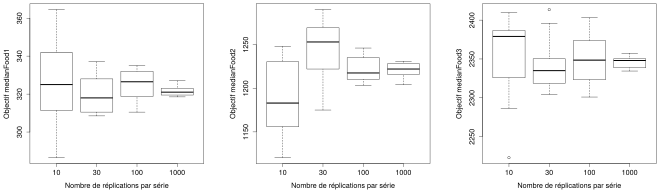
\includegraphics[width=1.0\linewidth]{ant_serie_stoch.pdf}
\end{figure}

Pour réaliser ce type de graphique, on réalise $10$ séries de $10$, de $30$, de $50$, de $100$ puis de $1000$ réplications pour un jeu de valeur de paramètres test fixé à $\{population = 125.0, diffusion-rate = 25.0, evaporation-rate = 25.0\}$. D'autres jeu de valeurs de paramètres donneraient probablement des résultats différents.

Dans le cas de l'exemple \textit{Ants}, on voit bien qu'en fonction du nombre de réplications, la valeur trouvée sur les objectifs ${medianFood1, medianFood2, medianFood3}$ est très variable. Si le nombre de réplications est trop faible, il est tout à fait possible que l'optimiseur sélectionne comme satisfaisantes des solutions candidates qui amènent le calcul d'une \textit{fitness} satisfaisante \enquote{une fois de temps en temps} ...

S'il n'est pas possible de réaliser le nombre de réplications idéales/suffisantes, ce qui est souvent le cas, alors il est conseillé de réévaluer régulièrement les solutions candidates retenues par l'optimiseur. C'est particulièrement important dans le cas des Algorithmes Evolutionnaires mobilisant une population de solutions candidates, car ceux-ci conservent et remobilisent les meilleurs individus entre les différentes itérations. Une fois entré dans cette population \enquote{par chance}, l'individu va continuer à fournir une descendance dont les capacités estimées sont biaisées.

Ce cas a été rencontré lors des expérimentations pour SimpopLocal. Ce modèle de simulation nécessite en effet l'exécution d'au moins $100$ réplications si on veut lisser correctement les erreurs sur les différents objectifs. Devant le nombre d'évaluations du modèle réalisé (plusieurs millions), seul $30$ réplications ont pu être faites pour chaque jeu de valeurs de paramètres. Un mécanisme spécifique à été intégré à MGO pour permettre la réévaluation aléatoire des meilleures solutions conservées par l'optimiseur (Algorithme Evolutionnaire) \autocite[193]{Schmitt2014}.

\end{testiv}


Différents degrés de dominance ont été développés, comme par exemple la notion de \textit{strong dominance} : $x_1$ domine fortement $x_2$ ($x_1 \succ \succ x_2$) si $x_1$ est strictement meilleur que $x_2$ sur tout ses objectifs.

\begin{table}[!h]
	\centering
	\begin{sidecaption}[Règle de dominance pour les points e et f]{Application des règles de dominance aux points $e$ et $f$. \\ \\
		   \begin{tabular}{>{$}l<{$}>{$}l<{$} >{$}l<{$}}
					\toprule
					 & f1 & f2 \\
					\midrule
					e      & 0.5    &  4   \\
					f      & 0.5    & 5,5  \\
					\bottomrule
			\end{tabular}\\ \\
			(a) $e \succ f$ car e est bien le meilleur sur au moins un des deux objectifs, et n'est pas pire sur aucuns des autres objectifs ($e \succeq f$ ) \\
			(b) f ne domine pas e car f n'est pas meilleur sur aucun des deux objectifs et il est pire sur au moins un des deux objectif}[tab:minipranking]

		\begin{minipage}{0.5\textwidth}
			\centering
			\subbottom[e est dominé par f ?\label{pranking_a}]{
				\begin{tabular}{>{$}l<{$}>{$}l<{$} >{$}l<{$}}
					\toprule
					    & f1 & f2 \\
					\midrule
					e \leq f & \text{true} & \text{true} \\
					e < f   & \text{false}  & \text{true} \\
					\bottomrule
				\end{tabular}
		 	}
		 \end{minipage}\hspace{1em}
		 \begin{minipage}{0.5\textwidth}
		 	\centering
			\subbottom[f est dominé par e ?\label{pranking_b}]{
				\begin{tabular}{>{$}l<{$}>{$}l<{$} >{$}l<{$}}
					\toprule
					  & f1 & f2 \\
					\midrule
					f \leq  e & \text{true} & \text{false} \\
					f < e  & \text{false}  & \text{false} \\
					\bottomrule
				\end{tabular}
			}
		\end{minipage}
  \end{sidecaption}
\end{table}

Pour bien comprendre comment se construit l'ensemble $X^*$ de solutions non dominées $x^* \in \mathbb{X}$ ,on peut étudier en détail dans le tableau \ref{tab:minipranking} comment la dominance se calcule entre les points $e$ et $f$, toujours tirés du tableau \ref{tab:pranking}.

Les solutions admises parmi le front de Pareto (voir figure \ref{fig:frontoptimal}) sont donc ici toutes celles qui ne sont pas dominées faiblement ($\succeq$), ce qui revient à exclure les points $f$ et $l$ du front optimum $\{a,b,c,d,e\}$ car ils sont dominés faiblement ($e \succeq f$); alors que dans le cadre d'une dominance forte ($\succ \succ$), ceux-ci auraient fait partie du front $\{a,b,c,d,e,f,l\}$. En effet si on prend toujours le cas de $e$ et $f$, la condition testant que $e$ est strictement meilleur que $f$ sur tous les objectifs n'est pas remplie.

%Cet ensemble de cardinalité forcément inférieure ou égale est qualifié \enquote{d'ensemble fort non dominé} (\textit{Strongly non dominated set}).

Le front de Pareto pour $\succ \succ$ est plus \textbf{grand} que le front de Pareto pour $ \succ $. Or $\succ \succ$ est \textbf{plus stricte} que $\succ$. Le raisonnement est contre-intuitif, par conséquent nous allons le dérouler plus en détail par la suite en observant de plus près le cas litigieux, c'est-à-dire pour le point $f$ et $l$, car $f_1 = e_1$

\pagebreak

On examine si $f$ doit être exclu de l'ensemble Front de Pareto $FP$ dans les deux cas, pour une dominance forte ($\succ \succ$) et une dominance faible ($\succeq$)

\medskip

\textbf{1) Dans le cas d'une dominance forte : }
\begin{align*}
     si f \notin FP & \Rightarrow \exists x \in FP \\
     & \text{tel que }  x \succ \succ f
\end{align*}

On teste tous les éléments de $FP$, le seul qui pose question est le point $e$, on pose donc la question suivante, est ce que $e \succ \succ f$ ?

\textbf{Non,} car $f_1(e) = f_1(f)$ , et donc $e$ ne domine pas fortement $f$. N'étant pas en mesure d'établir un ordre entre ces valeurs, il est impossible d'exclure $f$ de $FP$, et donc $ f \in FP_{\succ \succ}$

\medskip

\textbf{2) Dans le cas d'une dominance faible : }
On reprend la définition qui nous est donné, $ e \succeq f$ si
\begin{enumerate}[label=(\arabic*),labelindent=\parindent,leftmargin=*]
\item $ \forall_i \ e_i \leq f_i$
\item $ \exists_j \ e_j < f_j$
\end{enumerate}

\medskip

Or (1) est bien $True$ d'après le tableau \ref{pranking_a}, il est donc possible d'écrire $e_1 \leq f_1$ et $e_2 \leq f_2$. Le cas (2) est également $True$ car $e_2 < f_2$

\medskip

\textbf{Par conséquent}, le fait que (1) et (2) soit égal à $True$ permet, à la différence de la dominance forte, de discriminer $e$ par rapport à $f$, ce qui fait  que $e_2 \succeq f_2$. Donc $f \notin FP_{\succeq}$

\begin{table}[!p]

\begin{sidecaption}[Tableau résumé des fonctions objectifs, et de différentes valeurs de fitness associées]{Tableau de résultats des fonctions objectifs $f_1$ et $f_2$ pour un vecteur de solutions candidates $\{a \dotsc p\}$ dans l'espace des objectifs $\mathbb{Y}$, et résultat du \textit{Pareto Ranking}, intervenant ensuite dans le calcul de \textit{fitness} de différentes façons selon les algorithmes utilisés.}
	[tab:pranking]
	\centering
	 \subbottom[Graphique en deux dimensions des fonctions objectifs $f_1$ et $f_2$ du tableau ci-dessous.\label{pranking:a}]{
  		\includegraphics[width=.4\linewidth]{pareto_ranking_a.pdf}
  	}\qquad
	\subbottom[Tableau de données pour les solutions candidates des différents exemples.\label{pranking:b}]{
	\begin{threeparttable}
	\begin{tabular}{>{$}l<{$} >{$}l<{$} >{$}l<{$} >{$}l<{$} >{$}l<{$} >{$}l<{$}}
			\toprule
			\text{solutions candidates} & f_1 & f_2 & \text{dominé par} & v_1\tnote{1} & v_2\tnote{2} \\
			\midrule
			a      & 3.5    & 1    &  \varnothing & 1 & 1 \\
			b      & 3      & 1,5  &  \varnothing & 1 & 1 \\
			c      & 2      & 2    &  \varnothing & 1 & 1 \\
			d      & 1      & 3    &  \varnothing & 1 & 1 \\
			e      & 0.5    & 4    &  \varnothing & 1 & 1 \\
			f      & 0.5    & 4.5  &  \{e \}      & 2 & 2 \\
			g      & 1.5    & 4.5  &  \{d,e,f,h \} & 5 & 3 \\
			h      & 1.5    & 3.5  &  \{d \}      & 2 & 2 \\
			i      & 2      & 3.5  &  \{c,d,h \}  & 4 & 3 \\
			j      & 2.5    & 3    &  \{c,d \}    & 3 & 2 \\
			k      & 3.5    & 2    &  \{a,b,c \}  & 4 & 2 \\
			l      & 4.5    & 1    &  \{a \}      & 2 & 2 \\
			m      & 4.5    & 2.5  &  \{a,b,c,k,l \} & 6 & 3 \\
			n      & 4      & 4    &  \{a,b,c,d,e,h,i,j,k,o \} & 11 & 5 \\
			o      & 3      & 4    &  \{b,c,d,e,h,i,j \} & 8 & 4 \\
			p      & 5     & 4.5   &  \{a,b,c,d,e,f,g,h,i,j,k,l,m,n,o \} & 16 & 6 \\
			\bottomrule
	\end{tabular}
	\begin{tablenotes}
      \small
      \item[1] $v_1$ est une \textit{fitness} calculée sur la base du nombre de dominé $+ 1$, cf. une partie de calcul de fitness de l'algorithme MOGA de \textcite{Fonseca1993}.
      \item[2] $v_2$ est une \textit{fitness} calculée sur la base du calcul de fronts de l'algorithme NDS de \textcite{Goldberg1989}. L'algorithme est assez simple, on fait comme s'il s'agissait de peler un oignon. Au départ $r = 0$. On effectue un calcul de dominance sur une population complète $P$ (étape 1), puis on retire seulement les points non-dominés $P_{t+1} = P_{t} - P_{\{\varnothing\}}$ (étape 2) auxquels on attribue également un rang $r = r + 1$.  On recommence à l'étape 1 jusqu'à ce que tous les points possèdent un rang. Il existe également des variantes plus rapide de cet algorithme \autocite{Deb2001}.
    \end{tablenotes}
	\end{threeparttable}}
  \end{sidecaption}
\end{table}

\pagebreak

\begin{figure}[!htb]
	\begin{sidecaption}[Tracé d'un front de Pareto]{Tracé du front optimum à partir du calcul des individus non dominés, cf. l'ensemble vide $\varnothing$ dans le tableau \ref{tab:pranking}}[fig:frontoptimal]
		\centering
		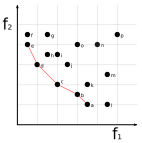
\includegraphics[width=.4\linewidth]{pareto_front.pdf}{
		}
  \end{sidecaption}
\end{figure}

Le front de Pareto n'est en général jamais entièrement couvert, cela pour diverses raisons :

\begin{itemize}
\item L'évaluation de la fonction à optimiser est souvent coûteuse, comme dans le cas de modèle de simulation dont l'exécution peut prendre jusqu'à plusieurs dizaines de minutes,
\item La zone d'exploration est volontairement bornée du fait des objectifs des expérimentateurs,
\item La stochasticité oblige l'exécution de nombreuses réplications d'une même évaluation,
\item On dispose de ressources finies, or l'espace du front est souvent continu et non borné en dehors des contraintes que l'on aura nous-mêmes fixées.
\end{itemize}

Selon \textcite[70]{Weise2011} et \textcite[19]{Zitzler1999a}, on peut s'aider dans cette tâche d'établissement d'un front de Pareto correct en étant attentif aux points suivants:

\begin{enumerate}
\item{\textbf{Proximité}} Les solutions découvertes doivent être les plus proches possibles du front de Pareto optimal.
\item{\textbf{Diversité}} Si le front optimal possible est trop large, la répartition des solutions \textit{spread} doit être maximisé sur toute la surface de celui-ci, si possible suivant une distribution uniforme.
\item{\textbf{Pertinence}} Les solutions découvertes doivent correspondre aux intérêts définis par le problème, et n'ont aucun intérêt si l'opérateur humain ne peut, ou ne sait les utiliser.
\end{enumerate}

On retrouve dans ces objectifs la tension entre exploration et exploitation, le front de Pareto devant être exploité de façon homogène, tout en garantissant à terme (et si possible le plus vite possible) la convergence vers une zone d'intérêt pour l'expérimentateur (voir figure \ref{fig:convergence_diversite}). Les métaheuristiques n'ayant pas d'apriori sur la forme de problème abordée, c'est dans l'originalité, la diversité des constructions proposées qu'une solution optimale et dédiée peut être trouvée. Il est donc très difficile de faire un listing des meilleures stratégies, et des meilleures combinaisons de stratégies permettant une sélection garantie des meilleurs candidats en fonction de ces objectifs, l'établissement de cette liste ne pouvant être que contextuelle d'un problème d'optimisation donné\Anote{no_free_lunch}.

Heureusement, un certain nombre de combinaisons, souvent éprouvées par de multiple tests sur des fonctions aux caractéristiques et difficultés soigneusement étudiées (ZDT, etc.), se démarquent par des capacités de résolution acceptable. C'est d'ailleurs souvent sur cette première base que se construisent ensuite les améliorations nécessaires à une réponse optimale, cela en partie grâce à la flexibilité des composantes caractéristique des métaheuristiques.

\begin{figure}[!htbp]
  \begin{sidecaption}[Comparaison entre deux fronts de Pareto, avec et sans maintien de la diversité]{Convergence et maintien de la diversité au sein du front de Pareto}[fig:convergence_diversite]
  \centering
  \subbottom[Un front de pareto sans maintien suffisant de la diversité.\label{subfig_convergence_diversite:a}]{
  	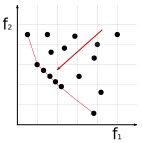
\includegraphics[width=.4\linewidth]{pareto_convergence_a.pdf}
  	}\qquad
  \subbottom[Un front de pareto avec maintien de la diversité.\label{subfig_convergence_diversite:b}]{
	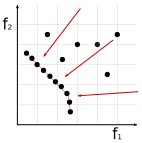
\includegraphics[width=.4\linewidth]{pareto_convergence_b.pdf}
  	}
 \end{sidecaption}
\end{figure}

\textit{Une fois défini cet ordre partiel entre les solutions candidates évaluées, sur quelle base l'optimiseur prend sa décision pour sélectionner les individus les plus prometteurs ? et comment celui-ci garantit l'évolution des solutions candidates selectionnées au regard des trois objectifs fixés ?}

Comme le dit de façon très claire,\textcite[94]{Weise2011} \foreignquote{english}{Such comparisons, however, only state whether one candidate solution is better than another one or not, but give no information on \textbf{how much} it is better or worse and \textbf{how interesting} it is for further investigation. Often, such a scalar, relative measure is needed.}

L'optimiseur n'ayant pas les capacités pour comparer des fonctions entre elles, c'est par l'attribution d'un scalarlaire caractérisant chaque vecteur $z^* \in \mathbb{Y}$ résultat de l'évaluation d'une solution candidate, que celles-ci vont pouvoir être départagées. On parle de \enquote{fonction d'utilité}, ou de \enquote{fonction \textit{fitness}} pour désigner cette opération de transformation dont le résultat $z$ est utile uniquement en se plaçant dans le référentiel de l'optimiseur. Il s'agit d'un classement relatif des solutions les unes par rapport aux autres, calculés indépendamment des valeurs prises par les fonctions objectives, et intégrant un certain nombre d'autres critères, définis en réponse aux exigences des trois objectifs déjà évoqués (respect de la diversité, qualité de convergence, pertinence vis-à-vis du problème).

Ainsi, un des tout premiers paramètres à intégrer dans le calcul de cette fonction \textit{fitness} tient évidemment dans le choix d'une stratégie adaptée pour tirer le meilleur parti des informations récoltées dans l'application de cet ordre partiel sur l'espace $\mathbb{Y}$. Là ou des algorithmes vont appuyer la sélection des solutions à partir d'un calcul de rang (je ne garde que les $n$ premiers rangs), d'autres vont le faire à partir d'un décompte des non dominés (je ne garde que les individus non dominés $< n$), à partir d'une profondeur (je ne garde que les $n$ premiers fronts), ou encore en mélangeant ces différentes informations (voir les calculs effectués dans le tableau \ref{tab:pranking}) A cela il faut également ajouter la diversité de choix à disposition dans la selection d'une dominance, par le changement de l'opérateur utilisé dans le calcul (\textit{weak dominance}, \textit{strong dominance}, etc.), ou même la relaxe de celui-ci (\textit{epsilon-dominance}). Des choix de première importance, car ils interviennent directement dans la construction de l'ensemble de solutions retenues.

%\pagebreak

\bigskip

\begin{testiv}{L'epsilon dominance par l'exemple}{}

Soit deux fonctions objectifs $f_1$ et $f_2$, et une population de $10$ solutions candidates parmi lesquels l'optimiseur ne peux choisir que les $5$ meilleurs valeurs pour formuler les prochaines solutions candidates à évaluer. Une fois triés par ordre descendant sur les deux objectifs, on vient bien que l'optimiseur s'est focalisé autour de $[25.00, 25.05]$.

\begin{figure}[H]
	 \centering
	 	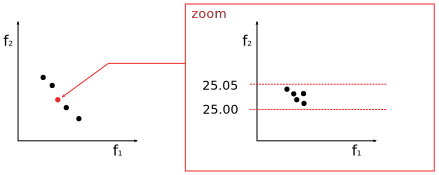
\includegraphics[width=0.8\linewidth]{epsilon_dominance.pdf}
	 	\label{fig:epsilon}
\end{figure}

La diversité à ce niveau de résolution doit paraître suffisante à l'optimiseur pour qu'il continue à sélectionner des candidats proches de $25$. Mais le gain est minime et cette pression sur $f_{2}$ masque peut être l'existence de meilleur compromis ailleurs.

\begin{table}[H]
	\centering
		\begin{minipage}{0.5\textwidth}
			\centering
			\subbottom[Valeurs triés pour $f_{1}$ et $f_{2}$ \label{epsilon_a}]{
			\resizebox{0.6\textwidth}{!}{%
				\begin{tabular}{@{}lll@{}}
				\toprule
				 & $f_{1}$ & $f_{2}$ \\ \midrule
				 1 & 9 & 25.00993 \\
				 2 & 9 & 25.01002 \\
				 3 & 10 & 25.01012 \\
				 4 & 10 & 25.01041 \\
				 5 & 11 & 25.01056 \\
				6 & 19 & 25.05121 \\
				7 & 20 & 16.3084 \\
				8 & 24 & 18.1433 \\
				9 & 26 & 18.2331 \\
				10 & 30 & 45.3212 \\ \bottomrule
				\end{tabular}%
		 }
		 }
		 \end{minipage}\hspace{0.2em}
		 \begin{minipage}{0.6\textwidth}
			\centering
			\subbottom[Mise en place d'un epsilon de $0.5$ \label{epsilon_b}]{
			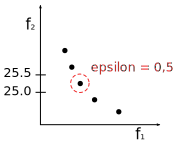
\includegraphics[width=0.8\linewidth]{epsilon_dominance_avec.pdf}
			}
		\end{minipage}
\end{table}

Une des possibilités est donc d'utiliser un epsilon de $0.05$ indiquant à l'optimiseur, au moment du calcul de la dominance, de considérer comme équivalentes les solutions dans ce radius autour d'un individu. Cela revient à relâcher la pression sur un des objectifs pour permettre à l'autre de s'exprimer. Dans notre exemple les $5$ premières solutions seront alors considérées comme équivalentes par l'optimiseur, et celui-ci se focalisera donc moins sur les micro-gains possibles sur $f_{2}$ au profit d'une plus grande diversité sur $f_{1}$. 

Une \textit{epsilon-dominance} a également été utilisée pour SimpopLocal, car un des objectif (population) était beaucoup trop sensible (voir annexe \ref{sec:simpoplocal}).

\end{testiv}

C'est donc dans l'espace des objectifs $\mathbb{Y}$ que se révèle la première information pertinente pour l'optimiseur, nous indiquant, peu importe la forme de l'une ou de l'autre des fonctions et le positionnement des points sur celles-ci, une première sélection de solutions parmi les solutions candidates évaluées sur laquelle l'effort de l'optimiseur doit porter en priorité.

Mais lorsque l'on reprojette les résultats du front de Pareto dans l'espace figurant la dynamique supposée de chacune des deux fonctions objectifs, on observe que la prise de décision basée sur le seul ordonnancement des solutions n'est pas suffisante pour garantir une selection optimale des meilleurs candidats à l'évolution (voir figure \ref{fig:mo_landscape}).

La forme des fonctions dans cette figure est représentée en pointillé car elle n'est qu'une description temporaire d'un paysage en partie inconnu, en attente d'être révisée par l'évaluation de nouveaux points. Le tracé d'un paysage ne se confond plus comme cela pouvait être le cas dans une optimisation mono-objectif avec la valeur prise par la fonction objectif, et doit maintenant intégrer un intermédiaire supplémentaire plus complexe qui est le calcul d'une fonction \textit{fitness}, et dont la formulation, dépendante de nombreuses stratégies, va modifier les solutions choisies dans le futur, et donc modifier la façon dont on va découvrir l'approximation de ce paysage, cela de façon indépendante aux objectifs choisis. \autocite{Weise2011}

\begin{figure}[!htbp]
	\begin{sidecaption}[Projection des individus extraits du front de Pareto dans l'espace des paramètres]{Projection du front de Pareto optimal (point \sqbox{tangoBlack1}), et des autres solutions candidates dominées (point \sqbox{tangoGrey1}) sur l'espace de variation du paramètre $x \in \mathbb{R}$, un schéma inspiré par \textcite[67]{Weise2011}
	\parbox{\marginparwidth}{
	\begin{enumerate}[label={},labelindent=0pt,leftmargin=*]
	      \item \sqbox{tangoBlue1} $f_{1}(x)$
	      \item \sqbox{tangoRed1} $f_{2}(x)$
	\end{enumerate}}\\
	Les fonctions $f_{1}(x)$ et $f_{2}(x)$ sont représentées en pointillé car elles sont inconnues de l'optimiseur, et ne servent que de repère au lecteur pour mieux comprendre comment un paysage caractérisant l'intersection des deux fonctions peut émerger durant l'optimisation, et pourquoi cela peut être intéressant d'intégrer son analyse à l'optimiseur.}[fig:mo_landscape]
	 \centering
	 	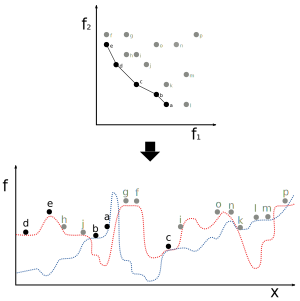
\includegraphics[width=0.8\linewidth]{multi_objective_landscape.pdf}
	\end{sidecaption}
\end{figure}

%on se rend également compte qu'un surplus d'information tiré de l'exploitation d'autres espaces pourrait être utile au choix de l'optimiseur

%\Anote{weise_multi2D}
Déjà beaucoup plus difficile à imaginer que dans l'exemple précédent de l'équation de Schaeffer, la re-projection des solutions candidates évaluées se fait sur un nouvel espace $\mathbb{G}$ (voir figure \ref{fig:relation_espaces}), qui inclut l'ensemble de tout les éléments $g \in \mathbb{G}$ pouvant être manipulés par les opérateurs de recherche à disposition de l'optimiseur \autocite[82]{Weise2011}. Un processus détaillé un peu plus tard dans cette section.

Dans notre cas $x \in \mathbb{R}$, on a donc un paramètre qui est manipulable et peut prendre une infinité de valeurs dans le cadre des contraintes définies pour $x$ (par exemple une valeur de 0 à 10 pour $x$)\Anote{remarque_resolution}. L'espace $\mathbb{G}$ contient la codification du problème, ce qui par exemple dans le cadre de simulation, se traduit pour chaque élément $g$ par l'attribution d'un vecteur de paramètres définissant les entrées de la simulation sur lequel l'optimiseur va pouvoir \enquote{jouer} pour optimiser les différentes fonctions objectifs.

La fonction $gpm : \mathbb{G} \to \mathbb{X}$ est une translation opérée lorsque les deux espaces sont de nature différente, par exemple pour passer d'un espace Binaire à un espace de Réels $\mathbb{B} \to \mathbb{R}$. Dans le cadre de simulations, les deux espaces sont souvent de nature similaire $\mathbb{G} = \mathbb{R}$. On pourra se référer à \textcite[86-88]{Weise2011} pour plus de détails.

\begin{figure}[!htbp]
	\begin{sidecaption}[Résumé des relations entres les différents espaces d'une optimisation]{Résumé des relations entre les différents espaces dans une optimisation}[fig:relation_espaces]
		\centering
		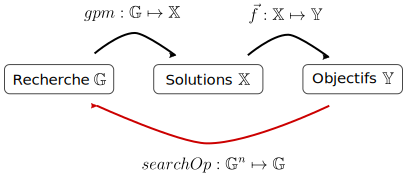
\includegraphics[width=.7\linewidth]{objectifsToSearchSpace.pdf}
  \end{sidecaption}
\end{figure}

%D'une part, l'observation de dynamiques en partie contraires sur ces deux fonctions $f_1$ et $f_2$ nous permet de constater encore une fois pourquoi un déplacement de l'optimiseur sur l'une ou l'autre des fonctions dirigé par la recherche d'un optimum n'a aucun sens.

L'opération de sélection des solutions candidates est souvent rattachée au processus de convergence. L'objectif de l'optimiseur est d'évaluer au mieux le potentiel de chacune des solutions durant cette phase de sélection pour intégrer et conserver les meilleurs éléments à son référentiel entre deux itérations. On imagine pourtant très bien l'effet que peut avoir une sélection trop restrictive sur le maintien de la diversité. C'est le cas par exemple si l'optimiseur ne décide de garder que le front de Pareto, on voit bien sur la figure \ref{fig:mo_landscape} à quel point la couverture de la dynamique des deux fonctions ressortirait considérablement appauvrie à la suite d'un tel choix. On en déduit que la frontière entre stratégies de convergence, et stratégies de maintien de la diversité doit être assez perméable pour garantir le choix de solutions candidates pertinentes en dehors du seul front de Pareto. \textcite{Zitzler1999a} retient par exemple parmi ces classes de stratégies celle s'appuyant sur le couple associant espace des objectifs et au choix la dominance, la densité, le temps, ou encore la chance. Ce sont des heuristiques qui vont intervenir en amont sur la qualité et la diversité des solutions candidates (par exemple les stratégies de \textit{sharing}, \textit{crowding}, etc.) qui peuvent ensuite être manipulées par les opérateurs de recherches de l'optimiseur.

Viennent ensuite les stratégies de recombinaison des solutions selectionnées, créatrices de nouvelles solutions candidates à évaluer. Un processus qui peut être là aussi rattaché tout autant au maintien de la diversité qu'à une volonté de convergence accrue. Il n'y a là encore aucune règle d'applications spécifiques, et tout dépend de l'objectif fixé de façon initiale ou au cours de l'expérimentation. Ainsi, certaines stratégies intégrées aux opérateurs peuvent être mis en place pour limiter une convergence trop rapide des solutions (\textit{premature convergence} généralement associé à une perte de diversité), alors que d'autres vont tenter d'accélérer cette convergence par la mise en oeuvre d'opérateur de recherche plus agressif, soit pour trouver le plus rapidement possible un minimum (ou maximum) local, soit car la topologie de l'espace des objectifs est difficile.

La sélection de candidats à la manipulation dans l'espace des objectifs $\mathbb{X}$ se réfère, une fois projetée dans cet espace $\mathbb{G}$, aux éléments $g$ accessibles à la manipulation par les opérateurs de recherche de la fonction $searchOp$. Chacun de ces opérateurs, dont le nombre et la nature est un paramètre de l'optimiseur, s'appuie sur la transformation d'une ou plusieurs solutions candidates dirigée par la création d'un nouvel élément $g$, dont on attend si possible un meilleur résultat à l'itération suivante. Un postulat très fort est posé par ce type de méthodes d'optimisation, l'introduction de petites variations sur les valeurs de l'espace de recherche est également censée apporter de petites variations dans l'espace des objectifs, que cela résulte en une amélioration ou en une dégradation de la qualité. Appelée \textit{strong causality}\Anote{note_strong}, cette propriété est évidemment dépendante de la forme prise par le paysage du problème (\textit{problem landscape}), et plus celui-ci est accidenté, rugueux, plus sa résolution est considérée comme complexe\Anote{note_weak}.

En relation avec cette observation, l'éclatement de cette population de solutions candidates évaluées sur le paysage nous permet de constater (voir la figure \ref{fig:mo_landscape}) à quel point la notion de distance entre les points paraît différente entre ces deux espaces. $f$ et $c$ apparaissent ici beaucoup plus proches d'un optimum global que $a$ et $b$, ces deux derniers étant pourtant plus proches de $c$ que $f$ dans l'espace des objectifs. On voit bien ici que la sélection de solutions candidates intéressantes peut intégrer d'autres informations utiles, en supplément de celles fournies par l'analyse de $\mathbb{Y}$, au travers de l'analyse de cet espace $\mathbb{G}$; et cela toujours afin de guider au mieux l'optimiseur dans la sélection des candidats à l'évolution. Un croisement du positionnement des individus $f$ et $c$ donnerait ainsi une bien meilleure valeur de $x$ à évaluer, probablement meilleure que celle d'un individu $a$ et $c$. Si la solution $f$ avait été éliminée sur le fait d'une sélection aux critères plus drastiques, c'est aussi la possibilité d'un croisement fructueux avec $c$ qui disparaît.

%A ces stratégies principales s'ajoute un autre ensembles de stratégies, dont certaines sont plus spécifiques, ou constitutives des types d'algorithmes utilisés. %Le maintien d'une diversité de solutions entre les itérations fait partie de ces stratégies qui font partie d'un set plus large de stratégies permettant de contrer l'émergence des différentes difficultés (stochasticité, topologie, etc.) caractéristique d'un problème de résolution unique.

%Généralement nommé \foreignquote{english}{Pareto Ranking}\Anote{utilisation_pareto_ranking} aussi nommé par Weise \foreignquote{english}{Prevalence Ranking}.

%\pagebreak
\bigskip

\begin{testiv}{De l'espace de paramètre à l'espace des objectifs sur l'exemple Ants}{}

\begin{center}
	 	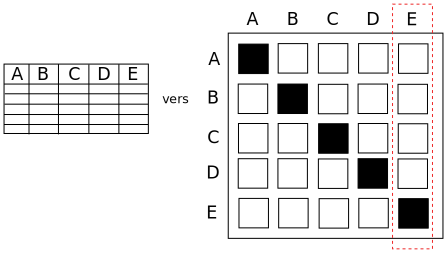
\includegraphics[width=0.6\linewidth]{matrix.pdf}
\end{center}

Un algorithme évolutionnaire a été utilisé pour trouver quels étaient les valeurs minimales de valeurs objectifs atteignables avec le modèle \textbf{Ants}. Autrement dit, on demande à l'algorithme d'optimisation de nous dire, dans la mesure du possible, quels sont les valeurs de paramètres (génome) nous permettant de minimiser au mieux la durée (trois fonctions objectifs ${f1,f2,f3}$) pour consommer le tas de nourriture 1, 2 et 3. Au bout d'un certain nombre d'itérations, cet algorithme nous propose un ensemble de solutions résultats incluant le front de Pareto, constitué ici de 3 dimension. Une vidéo de l'optimisation, les données au format csv, et le \textit{workflow} ayant permis d'arriver à ces résultats sont accessibles sur le site compagnon de la thèse (voir notes de lecture).

Comme il n'existe pas d'outil facile d'emploi permettant de sélectionner des points dans un espace en 3 dimensions tout en affichant simultanément les valeurs de paramètres auxquelles chacun de ces points est rattaché, nous allons nous contenter d'un autre outil en deux dimensions. Connu sous le nom de \textit{scatterplot matrix}, celui-ci permet de représenter un ensemble de points présents sous forme tabulaire classique vers la forme de matrice, comme représenté dans la figure ci-dessus.

Dans une forme interactive de cette représentation\Anote{scattrplot}, la sélection à la souris d'un ensemble de points met automatiquement en lumière la position de ceux-ci dans l'ensemble de la matrice. Dans notre cas, à chaque point sont associées les valeurs de paramètres suivantes $(diffusion-rate,evaporation-rate, medianFood1, medianFood2, medianFood3)$ Cette représentation permet d'explorer la relation entre l'espace des objectifs et l'espace des valeurs de paramètres en mettant tout sur le même plan 2D. Cette exercice d'analyse, encore faisable en deux dimensions, devient un peu plus difficile à réaliser à chaque fois que l'on ajoute des paramètres ou des objectifs. Afin de ne pas encombrer ce chapitre par des dizaines de matrices, j'ai choisi de réunir dans un seul et même schéma les différentes sélections (voir la zone encadrée de pointillé rouge dans la matrice) en prenant pour axe $x$ de référence l'objectif $f3$ minimisant la durée pour épuiser le tas de nourriture 3 le plus éloigné du nid.

\begin{center}
	\includegraphics[width=0.9\linewidth]{resume.jpg}
\end{center}

Il ne faut pas oublier que cette analyse se fait sur une population de solutions évaluées stabilisée, elle est donc très resserrée autour de certains comportements clefs. Des frontières qui renseignent le modélisateur sur les contradictions auxquelles l'algorithme d'optimisation doit faire face pour minimiser ces trois objectifs à la fois. On voit bien que les écarts sont très différents selon les objectifs, ce qui peut parfois poser problème à l'optimiseur.

\begin{itemize}[nolistsep]
	\item Dans la colonne (a), on s'intéresse à un premier cluster de valeurs d'évaporation compris entre $[5.5, 10]$. On voit que pour cette sélection le taux de diffusion est très étalé, entre $[20, 80]$, ce qui indique le peu d'impact de celui-ci dans cette dynamique. Quelque soit la valeur dans cet intervalle, le modèle est toujours proche de valeurs égale à $800$ à +/- $100$ près pour \textit{medianFood3}. S'il y a bien une forme de stabilité exprimée pour ce troisième objectif, le deuxième objectif est par contre beaucoup plus sensible car sa valeur peut varier entre $[300, 550]$. De la même façon, la valeur de l'objectif \textit{medianFood1} est très étalée entre $205$ et $230$. On pourrait qualifier de comportement moyen ce profil, car il ne donne pas les pires résultats sur l'objectif \textit{medianFood3}, il donne des résultats assez resserrés entre $[200, 230]$ sur l'objectif \textit{medianFood1}. Pour l'objectif \textit{medianFood2} par contre, c'est moins clair, il semble y'avoir un effet de seuil.
	\item On sélectionne un cluster qui partage certaines valeurs avec le précédent, sur les valeurs d'évaporations comprises entre $[5, 6]$. On voit qu'avec ces valeurs-là, il est possible d'atteindre des valeurs minimales sur l'objectif \textit{medianFood3}, aux environs de $600$. La lecture de $diffusion-rate$ nous indique qu'il faut se concentrer sur des valeurs comprises entre $[15, 40]$ pour observer cet effet. Des valeurs qui se chevauchent avec la tranche donnée précédemment dans la colonne (a), entre $[20, 60]$. Il faut que ces deux conditions réunies (taux d'évaporation $< 6$ et taux de diffusion compris entre $[20, 40]$) pour qu'une valeur minimale puisse etre atteinte sur l'objectif \textit{medianFood3}. Dans cette configuration, les résultats sur l'objectif \textit{medianFood1} sont moins bons que précédemment, l'optimiseur a du faire un compromis. La valeur sur l'objectif \textit{medianFood2} est stable autour de $400$, alors dans la colonne (a) ce n'était pas le cas. Le point de tension semble donc plus être entre l'objectif \textit{medianFood1} et \textit{medianFood3}, ce qui semble assez logique vu la configuration des tas de nourriture 1 et 3. Il faut toutefois aussi relativiser la dégradation des performances sur cet objectif \textit{medianFood1}, elles sont minimes entre (a) et (b) (entre $0$ et $50$ d'écart max avec (a)), surtout en comparaison du gain obtenu sur l'objectif \textit{medianFood2}, devenu plus stable, et \textit{medianFood3} moins long de $200$ vis à vis de (a). Cette configuration de paramètres paraît etre la plus intéressante pour le moment, tout dépend de l'importance accordée par le modélisateur à la dégradation de performance sur l'ojectif \textit{medianFood1}.
	\item La colonne (c) montre de toute évidence que les candidats les meilleurs sur l'objectif \textit{medianFood1} $< 200$, sont aussi potentiellement les plus mauvais sur l'objectif \textit{medianFood2} et \textit{medianFood3}. Plus on se rapproche de l'intervalle $[80, 100]$ sur la diffusion, en restant au delà de $10$ sur $evaporation-rate$, et plus les résultats sur l'objectif \textit{medianFood2} et \textit{medianFood3} se dégrade. Toutefois par recoupement avec ce que l'on a observé dans la colonne (a), il semblerait qu'un point se détache du lot dans ce paquet, et permette d'obtenir une valeur de $800$ sur l'objectif \textit{medianFood3}, environ $350$ sur l'objectif \textit{medianFood2}, et $ < 200$ sur l'objectif \textit{medianFood1}. Toutefois, et c'était quelque chose que l'on avait déjà ressenti dans l'analyse de la colonne (a), l'objectif \textit{medianFood2} a l'air assez sensible sur l'un ou l'autre de ces intervalles (passe de $350$ à $500$). Cela constitue un autre jeu de valeur de paramètre intéressant, si on n'est pas pret à sacrifier une partie de la performance obtenue sur l'objectif \textit{medianFood1}.
	\item La colonne (d) s'intéresse au groupe de valeurs $[300, 400]$ sur l'objectif  \textit{medianFood2}. On voit que la sélection recoupe clairement ce que l'on a vu dans les colonne (a) et (b). Si on veut obtenir une valeur pour l'objectif \textit{medianFood3} entre $[600, 800]$, et une valeur aux alentours de $400$ pour l'objectif \textit{medianFood2}, il suffit de prendre une valeur au hasard dans cet intervalle de valeurs comprises entre $[15, 80]$ pour la diffusion, et $[5, 10]$ pour l'évaporation.
\end{itemize}

\end{testiv}

% Ou introduire la notion d'individu ?

\pagebreak

\begin{figure}[ht]
	\begin{sidecaption}[Résumé d'une optimisation]{Résumé simplifié du déroulement d'une optimisation selon \textcite[109]{Weise2011}}[fig:resume_opti]
		\centering
		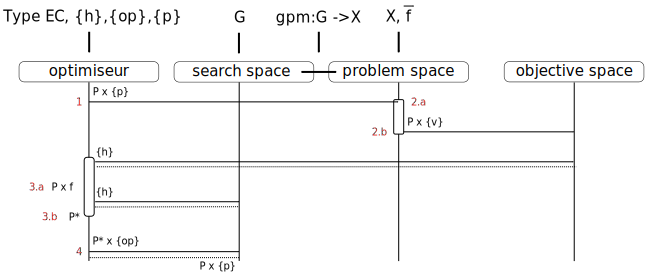
\includegraphics[width=\linewidth]{espace_resume.pdf}{
		}
  \end{sidecaption}
\end{figure}


La description des étapes de la figure \ref{fig:resume_opti} sont les suivantes :

\begin{itemize}[label=\textbullet]
	\litem{1} Une première population $P \in \{1 \dotsc n\}$ de vecteurs paramètres ${p}$ est générée par l'optimiseur ou introduite par l'expérimentateur, puis soumis à évaluation.
	\litem{2.a} La fonction à optimiser est évaluée autant de fois qu'il y a de vecteurs ${p}$
	\litem{2.b} Les fonctions objectifs $\vec{f}$ sont calculés, ce qui permet de créer autant de vecteur ${v}$, contenant chacun le résultats des fonctions après évaluation, qu'il y a de $P$ évalué. Ces vecteurs $P(v)$ peuvent être positionnés dans un espace des objectifs $\mathbb{Y}$
	\litem{3.a} Le calcul de \textit{fitness} $f$ est effectué pour chaque élément de $P$ en utilisant les informations rapportées par un ensemble d'heuristiques sur $\mathbb{Y}$ et/ou $\mathbb{G}$
	\litem{3.b} A partir du calcul de cette \textit{fitness} $f$ pour chacun des éléments de $P$, on selectionne les $P^*$ meilleurs éléments.
	\litem{4} A partir d'un ensemble d'opérateur ${op}$ on va générer de nouveaux vecteurs de paramètres $P(p)$, qui va constituer le nouveau jeu de solution candidates à évaluer à l'étape (1), et dont on espère qu'elles seront si possible meilleures que les précédentes.
\end{itemize}




%\hl{Manque la notion d'invididu = fitness + genotype + phenotype}





% Penser à dire qu'il y a plusieurs stratégies de comparaison autre que Pareto ?


%Si on transfère ce langage neutre au vocabulaire que l'on peut trouver courrament dans l'EC, alors l'espace des solution devient le \textit{phenome}, et le point de cet espace qui correspond à la solution candidate devient un \textit{phenotype}.


%Dans notre étude, l'objet à optimiser ne se réfère pas à une expression mathématique, mais à un modèle de simulation, sur lequel on va déterminer un ensemble de critères qui vont faire figure d'équivalent de ces fonction objectives. Dans ce cas d'utilisation, l'optimisation est plus souvent employé comme une forme de calibration inversé \autocite{Grimm2011}, dans laquelle on cherche à déterminer si il existe un ou plusieurs jeu de valeur de paramètres du modèles de simulation respectant la plage de valeur viable empiriquement qui permettent de maximiser l'obtention d'un ou de plusieurs critères experts. Il est plus parlant dans notre cas de désigner l'espace de recherche comme l'espace des paramètres.

La branche des métaheuristiques EC que nous allons étudier plus spécifiquement s'appuie sur l'observation de phénomènes naturels, comme l'évolution, ou l'organisation, pour la construction et la mise en oeuvre d'algorithmes mimant certaines propriétés intéressantes de ces processus, cela sans être rattaché à une contrainte de réalisme biologique.

\subsection{Les métaheuristiques bio-inspirées, la branche des Algorithmes Evolutionnaires}
\label{ssec:EA}

\subsubsection{Un rapide historique de la discipline}
\label{sssec:historique_EA}

On a rapidement décrit dans les annexes \ref{chap:double_foyer_sma} abordant le thème de l'\textit{Artificial Life} les deux voies qu'il était possible d'emprunter dans l'intérêt porté sur la définition du processus naturel d'évolution.

Il existe en effet au moins deux façons aujourd'hui d'introduire des développements informatiques se rapportant à ce processus évolutif. D'un côté, les tentatives de reproduction plus ou moins fidèles des différents mécanismes à l'oeuvre dans le processus d'évolution mettent en avant un objectif de compréhension, alors que la focalisation sur ces mêmes mécanismes pour leur seule capacité d'apprentissage tend à s'éloigner de la réalité biologique pour s'orienter plus vers le développement d'algorithmes désignés comme métaheuristiques. Autrement dit, là ou des chercheurs vont tenter de reproduire au mieux le processus d'évolution dans ce qu'il a de créatif, de non optimisé, de coévolutif car construit par\Anote{note_pattee_semantic_closure} et avec l'environnement, d'autres vont reprendre ce même processus en vue d'une évolution si possible bornée et dirigée par la résolution efficace d'un ou de plusieurs objectifs définis de façon fixe et extrinsèque \autocites{Taylor2001, Taylor2012}.

Lorsqu'on s'intéresse de plus près à la littérature scientifique de ces algorithmes regroupés depuis Fogel sous le terme d'\foreignquote{english}{Evolutionary Computation} (EC), on constate pour toute une partie des publications une de-contextualisation complète de leur utilisation. La question d'une similitude initiale avec le vivant n'étant le plus souvent évoquée que pour illustrer des racines historiques éloignées, alors qu'une meilleure connaissance de cette histoire pourrait au mieux participer d'une amélioration des algorithmes, et au pire au moins éviter la persistance de certains malentendus \autocite{DeJong1993a}. Ce qui peut apparaître comme une forme de surspécialisation est en quelque sorte le prix à payer d'une évolution de la discipline avant tout dirigée par une communauté de chercheurs informatiques motivés par la recherche d'algorithmes performants et d'applications génériques.

Si aujourd'hui on peut observer un tel cloisonnement, un regard sur l'histoire de la discipline tend à montrer tout l'inverse, car nombreux sont les pionniers ayant développé des intérêts simultanés pour ces deux approches : les expériences très longtemps restées inconnues du mathématicien Barricelli dès 1954\Anote{barricelli_multi_utilisation}, l'approche du généticien \textcite{Fraser1957} qui décrit et simule l'évolution de population génétique dès 1957\Anote{fraser_comment}, les travaux de Pattee et Conrad avec EVOLVE à la fin des années 1960 \autocite{Conrad1970}, les algorithmes génétiques\Anote{holland_multi_utilisation} de Holland, un élève de Burks, un scientifique dont on a indiqué qu'il était proche de Von Neumman.

Il existe toutefois une littérature scientifique parallèle qui continue de motiver la rencontre autour de disciplines scientifiques ayant un intérêt pour la recherche en \textit{Artificial Life}. C'est le cas par exemple de la biologie, ou de l'écologie \autocite{Hamblin2013} qui organisent autour de publications transverses la réflexion sur la reintroduction des outils tels qu'ils sont développés en informatique, entraînant de fait aussi la création et l'évolution de ces derniers \autocite{Hogeweg2011}. C'est également le cas en biologie, ou on imagine l'importance que peuvent avoir les travaux de \textcites{Taylor2001}[221]{Taylor1999} pour la mise en oeuvre de modèles de simulation dirigés vers l'émergence \enquote{créative} de nouveaux phénotypes dans un environnement ouvert \autocite[33]{Taylor1999}. Une critique récurrente adressée aux modèles d'auto-organisation actuels \autocite{Pumain2003}, encore incapables de simuler l'émergence de nouvelles structures, de nouvelles entités de façon crédible. Une autre forme de relation entre les deux approches est également envisageable dans certaines disciplines, comme en écologie, où celles-ci peuvent parfaitement se côtoyer :
\foreignblockquote{english}[\cite{Dorin2008}]{The first of these requires the application of the evolutionary process in much the same way as it has been traditionally applied within A-Life: as a means to dynamically adjust agent parameter values to support their viability and reproduction within the virtual environment. [...] The second approach we suggest employs artificial evolution to match simulation patterns against data gathered from the level of specific species up to data concerning specific ecosystems. Once the parameters of the system have been optimised so as to reproduce the patterns observed in field data, the evolution algorithm is turned off. The model may then be employed to answer questions relating to the specific ecosystem and species that it represents. Unfortunately it may not then be used to study the evolution of these specific species in specific environments. This is a shortcoming of the artificial evolution algorithm (it does not model real evolution in detail) that would be worth overcoming.}

Le lecteur souhaitant obtenir une vue plus globale des différents concepts et ramifications disciplinaires réunies sous le terme parapluie d'\textit{Artificial Life} peuvent se référer à l'article d'\textcite{Aguilar2014} qui concentre un grand nombre d'entrées bibliographiques essentielles pour aborder les entrées de cette thématique dans chacune des disciplines. On trouvera également une description plus précise sur l'histoire commune de ces deux voies de recherches, telles qu'elles sont perçues par les acteurs historiques de l'EC, dans les ouvrages de \autocites{DeJong2006a, Fogel1998, Fogel2006a, Fogel2006b, Back1996, Back1997}.

Dans cette section, c'est bien la deuxième branche de recherche qui est suivie, celle visant l'\enquote{optimisation}. Les développements tels qu'ils sont abordés ne se mesurent donc plus en fonction d'un critère de réalisme biologique, mais en fonction de critères informatiques et mathématiques se rapportant plus à la capacité de résolution des algorithmes, et aux supports de mise en oeuvre et de mesure de ces derniers : rapidité, diversité, robustesse, qualité, etc.

\textcite{DeJong2006a} retient trois foyers importants pour le développement de cette deuxième branche dans les années 1960, la \textit{Technical University} de Berlin avec Rechenberg, Biernet et Schwefel \autocite{Beyer2002}, UCLA à la même période avec Lawrence J. Fogel, et l'université du Michigan avec John Holland.

De ces trois branches vont émerger au cours des années 1970 ce que \textcite{DeJong2006a} qualifie comme des \foreignquote{english}{Evolutionary Algorithms (EA)} canoniques. Autrement dit, ce sont des algorithmes matures, qui ont prouvé leur capacité à produire des solutions dans un contexte précis : \foreignquote{english}{Evolutionary Programming (EP)}, \foreignquote{english}{Evolution Strategy (ES)}, \foreignquote{english}{Genetic Algorithm (GA)}

Ils vont représenter chacun le foyer d'un développement qui va s'accélérer dans les années 1980, avec l'amorce d'une popularisation de ces techniques permises entre autres par l'avènement de capacités de calcul plus conséquentes et la reconnaissance de l'efficacité de ces algorithmes pour la résolution de problématiques industrielles plus concrètes. L'ouvrage de synthèse écrit par \textcite{Goldberg1989} contribue de façon très importante à cette diffusion, et constitue également un apport théorique important dans la naissance de la branche multi-objectif de cette discipline.

Les années 1990 vont quant à elles consacrer la rencontre et l'unification de ces différentes approches restées jusqu'alors assez indépendantes si on en croit \textcite{DeJong2006a}. De cette confrontation naît la reconnaissance d'un seul terme fédérateur, l'\textit{Evolutionary Computation (EC)} motivant alors la création de nouvelles conférences et de nouveaux journaux structurant cette nouvelle discipline. C'est aussi à partir de cette période que l'on observe la mise en place d'une hybridation accélérée entre les différentes approches qui s'accompagne d'une forme de remise à plat théorique et l'émergence d'un cadre de réflexion unifié. \autocites[23-31]{DeJong2006a}{Back1997}

Si on se concentre plus précisément sur la branche multi-objectif de la discipline, la première introduction théorique d'une stratégie s'appuyant sur le calcul de l'optimum de Pareto pour définir un classement original des solutions évaluées est présenté à la page 197 de \textcite[197]{Goldberg1989}. Cette technique nommé \textit{Non Dominated Sorting} (NDS) \autocite[40-43]{Deb2001}, probablement la plus efficace et plus célèbre, sera reprise et implémentée presque dix ans plus tard en 1994, dans l'algorithme célèbre NSGA (Non dominated Sorting Algorithm) de Deb et Srinivas.

Les travaux de \textcite{Goldberg1989} ont influencé toute une génération de chercheurs à partir de cette simple ébauche théorique de tri basé sur la dominance de Pareto, et nombreux sont ceux qui se sont par la suite appuyés \autocite[175, 235]{Deb2001} sur les informations du calcul de dominance pour développer diverses stratégies d'attribution de \textit{fitness}, comme MOGA \autocite{Fonseca1993}, NPGA (Horn et Nafpliotis 1994), NSGA \autocite{Srinivas1994}, et bien d'autres \autocite[14]{Zitzler1999a}. Ce que l'on peut considérer comme la génération suivante d'algorithmes, que \textcite{Coello2006}\Anote{coello_note} fait démarrer avec l'apparition de l'élitisme\Anote{note_elitisme}, est plus axée encore sur l'efficacité de ces derniers avec notamment l'ouverture d'une branche de recherche développant des métriques de performance, et de nouveaux standards de mesures \autocites{Coello2006, Zitzler2003,Huband2006}, dont on s'aperçoit qu'elles sont devenues nécessaires pour comparer correctement les algorithmes entre eux \autocite[14-15]{Zitzler1999a}. Parmi ces nouveaux algorithmes, devenus depuis canoniques, on trouve PAES (Knwoles and Corne 2000), SPEA \autocite{Zitzler1999b}, ou encore NSGA 2 \autocite{Deb2000a}, etc. On trouve à ce sujet un état de l'art et des exemples de calculs à la main pour ces différents algorithmes dans un des premiers et très bon ouvrage de synthèse de \textcite{Deb2001}, aux chapitres 5 et 6. Il est toutefois à noter, comme le fait déjà Golberg en 1989, que cette problématique de recherche d'une solution à un problème multi-critères, puis multi-objectifs est d'origine bien plus ancienne, et a pu servir de support à la mise en oeuvre de techniques plus ou moins similaires à celle de Pareto. Ainsi, les premières traces en EA d'un intérêt théorique et parfois pratique de ces problèmes semblent remonter à Box et Draper (1957), Fogel (1966), Rosenberg (1967) \autocite[174-175]{Deb2001}. Mais la première implémentation informatique est en général attribuée à David Schaffer, avec son travail de thèse (1984) et l'implémentation de l'algorithme d'optimisation VEGA (\textit{Vector Evaluated Genetic Algorithm}) \autocite{Schaffer1985}. Un autre état de l'art sur l'optimisation multi-objectifs s'appuyant sur Pareto en dehors des techniques purement évolutionnaire est également possible. C'est grâce à l'existence de ce cadre formel mathématique permettant la description d'un problème d'optimisation, tel que nous l'avons un peu abordé dans la section précédente en s'appuyant sur les écrits de \autocite{Weise2011}, que \textcite[50-79]{Deb2001} indique par exemple comment certaines de ces stratégies hors EC ont été pour certaines également transférées avec plus ou moins de succès aux EA \textcite[171-237]{Deb2001}.

Enfin on notera qu'il existe également une autre classe proche d'algorithmes d'optimisation basée sur une observation des mécanismes naturels, celle-ci n'étant plus basée sur la métaphore évolutive par reproduction (même si l'hybridation est envisageable), mais sur les capacités d'organisation et d'auto-organisation observées chez certains animaux comme les fourmis, les abeilles. Ces comportements ont d'abord inspiré les développements de plateformes informatiques adaptées à l'émergence de ce type de comportements, avant d'être repris et utilisé de façon beaucoup plus abstraites par la suite pour résoudre des problèmes d'optimisation. Aujourd'hui regroupées sous le terme de \foreignquote{english}{Swarm Intelligence}, ce sont par exemple les algorithmes PSO (Particle Swarm Optimization), ACO (Ant Colony Algorithms), ABC (Artificial Bee Colony), etc.

\subsubsection{Les principes sous-jacents aux Algorithmes Evolutionnaires (EA)}
\label{ssec:principesEA}

Pour illustrer, formaliser et capitaliser sur cette capacité d'adaptation  permise par l'hétérogénéité et la grande flexibilité structurelle de ce type d'algorithmes, \textcite[49]{DeJong2006a} a considéré la mise en oeuvre d'un modèle conceptuel plus abstrait capable d'englober dans sa description les mécanismes des trois versions canoniques GA, ES et EP. Les concepts clefs qui se dégagent d'une telle prise de distance peuvent ainsi être repris non seulement pour décrire les versions canoniques, mais également pour développer de nouvelles variantes ou extensions d'algorithmes.

Les éléments communs retenus sont les suivants :

\begin{itemize}
\item Une population de taille constante $m$ évolue au cours du temps
\item La population courante est utilisée comme une source de parents pour produire une progéniture (\textit{offsprings}) de taille $n$
\item La population étendue ainsi constituée est réduite de $m + n$ à $m$ individus.
\end{itemize}

Une telle boucle évolutive ainsi maintenue sur plusieurs générations successives, lorsqu'elle est contrainte par des fonctions objectifs explicites, a clairement pour horizon la constitution d'une population de solutions idéales pour la résolution d'un problème donné. 
Encore une fois, il est important ici de rappeler que ces techniques évolutionnaires \textbf{ne sont pas bornées à cette seule fonction d'optimiseurs} \autocites{DeJong1993a}[262]{Weise2011}\Anote{weise_natural}, et un regard sur l'historique de ces techniques est là pour en attester (voir annexe \ref{sec:vie_artificielle}).

Une autre représentation, encore plus claire, est donnée par \textcite[254]{Weise2011} dans la figure \ref{fig:S_evolution}. On ne détaillera pas beaucoup plus chacune de ces étapes par la suite, pour plusieurs raisons : (a)elles sont documentées de façon exhaustive depuis plusieurs décennies, (b) les principaux concepts de l'optimisation et des métaheuristiques multi-objectifs ont été avancés de façon simplifiée dans la section précédente, et le lecteur curieux d'explorer plus en avant les spécificités propres aux différents classes d'algorithmes évolutionnaires pourra se référer à l'ouvrage de \textcite{Weise2011} (voir le tableau \ref{tab:ptraduction}), (c) on se concentre plus par la suite sur la création du support logiciel permettant justement de masquer cette complexité pour accéder à toute la puissance de ces techniques sans être un expert du domaine.

\begin{figure}[htbp]
	\begin{sidecaption}[Cycle d'évolution générique d'un Algorithme Evolutionnaire (EA)]{Cycle générique proposé par \textcite[211]{Weise2011} pour caractériser les différentes étapes constitutives d'un algorithme évolutionnaire}[fig:S_evolution]
	  \centering
	 \includegraphics[width=1.0\linewidth]{evolution_weise.jpg}
	  \end{sidecaption}
\end{figure}

\pagebreak

% En général puis recentrage sur les détails ?
\paragraph{Les avantages et les inconvénients d'une terminologie spécifique}

En 2014 une publication sur le blog du spécialiste de la discipline Thomas Weise's\Anote{billet_weise} revient longuemment sur les problématiques de ce vocabulaire inspiré par la biologie et ancré dans les différentes branches composantes l'EC. Il retient quatre problématiques dans l'usage de cette terminologie, parmi lesquelles l'incompatibilité des terminologies entre les différentes branches, la dissonance entre la terminologie et la réalité d'application des algorithmes, le fait que l'optimisation au sens naturel n'est pas forcément une bonne optimisation, le fait également que cette terminologie sonne comme anti--professionnelle\Anote{note_pengouin}. Le plus grand problème étant dans ce cadre l'invention de néologisme ne faisant référence ni au domaine biologique, ni au domaine informatique. Ce n'est pas la seule voix à se faire entendre sur ce sujet, comme l'article de \textcite{Sorensen2013b} qui pointe clairement les dérives néfastes associées à l'usage systématique et surtout non réellement argumenté de nouvelles analogies ou métaphores, que celle-ci soit biologique ou pas ...

Si la perspective d'un changement d'annotation et de vocabulaire est probablement conçue comme une étape majeure dans la progression et l'unification d'une discipline depuis quelques années déjà sur la voie de la maturité, Weise tout en prônant au maximum la bonne parole continue comme beaucoup d'autres à utiliser cette terminologie \autocite{Weise2011}, très ancrée dans un folklore qui tient à l'historique de la discipline. La librairie logicielle MGO décrite par la suite s'appuie elle aussi sur cette terminologie, aussi nous n'utiliserons donc les terminologies alternatives proposées par Weise que sous forme de complément, afin de ne pas introduire trop de distance entre les termes décrivant les algorithmes dans ce manuscrit et la réalité du programme tel qu'il est conçu pour le moment.

\begin{table}[!htbp]
\begin{sidecaption}[Tableau de correspondance entre les notations biologiques et génériques de l'optimisation]{Tableau de correspondance entre les notations à consonances biologiques et les notations plus génériques liées à l'optimisation, lorsque celles-ci existent. Une traduction appuyée sur la section précédente, et les travaux de \textcite{Weise2011}}
	[tab:ptraduction]
	\centering
	\resizebox{1.0\textwidth}{!}{%
	\begin{tabular}{ll}
		\toprule
		générique & biologique (FR)\\
		\midrule
		Espace du problème ($\mathbb{X}$) & Phénome \\
		Espace de recherche ($\mathbb{G}$)   &  Génome \\
		Point dans un espace de recherche ($g \in \mathbb{G}$) & Génotype \\
		Solution candidate, Point dans un espace de solutions ($x \in \mathbb{X}$) & Phénotype \\
		Opérateurs de recherches ($searchOp$) & Reproduction \\
		Opérateur de recherche Unaire & Mutation \\
		Opérateur de recherche Binaire & Crossover \\
		Itération & Génération \\
		?  & Progéniture (\textit{Offsprings}) \\
		?  & ? \textit{Mating pool} \\
		\bottomrule
	\end{tabular}%
	}
  \end{sidecaption}
\end{table}

\paragraph{Les avantages et les inconvénients des EA}

Ces deux listes comparant les avantages et les inconvénients des algorithmes évolutionnaires sont tirés des ouvrages de \textcites{Deb2001, Fogel2000, Back1997}[104,105]{DeJong2006a} mais également \textcites{Diplock1996,Openshaw1988} qui ont exploré ces techniques en géographie.

\begin{enumerate}[label=(\alph*),labelindent=\parindent,leftmargin=*]

	\item évaluation d'une population entière par génération, ce qui n'est pas le cas de nombre de techniques fournissant une seule solution par exécution d'algorithme.
	\item facile à paralléliser, une propriété étudiée très tôt \autocite[444]{Alba2002}.
	\item ne demande a priori aucune connaissance de la forme du paysage à parcourir, même si en réalité cette connaissance est un plus pour bien choisir et paramétrer les métaheuristiques.
	\item applicable à des problèmes continus, discrets, ou les deux.
	\item ne demande pas forcément de repartir de zéro entre chaque analyse en comparaison à d'autres algorithmes.
	\item le nombre de degrés de liberté accessible pour modifier une métaheuristique est important, ce qui augmente les chances de trouver une combinaison adaptée à un problème complexe donné.
	\item les principes de mise en oeuvre sont relativement faciles à comprendre
    \item efficace, même sous une forme canonique.
    \item capacité à explorer de très larges espaces de recherche.
\end{enumerate}

Les désavantages, limitations :

\begin{enumerate}[label=(\alph*),labelindent=\parindent,leftmargin=*]
	\item la dynamique de fonctionnement reste opaque, et elle n'est souvent pas tractable mathématiquement.
	\item la stochasticité demande la mise en oeuvre de réplication.
	\item pas de garantie de trouver un optimum global.
	\item le nombre de degrés de liberté demande une certaine forme expertise pour en tirer le meilleur parti, la construction d'un EA optimal pour un problème donné étant progressif, incrémental.
    \item trop facile à comprendre, il en résulte une certaine illusion quant aux capacités \enquote{magiques} de ce type d'algorithme.
    \item necessite une source conséquente de puissance pour réaliser de grands nombres de calculs en parallèle.
    \item les performances se dégradent avec l'augmentation de l'espace de recherche (dimensionnalité) ou le nombre d'objectifs (on touche les limites de l'approche Pareto) \autocite[24]{Zitzler1999a}.
\end{enumerate}

%\hl{2 paragraphe qui suivent à replacer au bon endroit}

L'optimisation de paramètres est un domaine d'application reconnu des EA du fait aussi de la facilité de \textit{mapping} entre un vecteur de paramètres et un génome \autocite[83]{DeJong2006a}. Cette branche spécifique des EA est également celle qui est à la fois la facile d'accès en terme de compréhension pour les débutants tout en restant également suffisamment flexible et efficace pour convenir à notre utilisation. Certains des désavantages évoqués ont également des conséquences plus limitées dans le cadre de nos objectifs. En effet, pour le profil d'\enquote{utilisateur modélisateur} que nous ciblons, la garantie d'un optimum global n'est pas la priorité immédiate en comparaison de l'importance d'accéder rapidement à des premiers résultats. Le premier EA canonique/ générique utilisé pourra de toute façon être amélioré, restructuré dans un deuxième temps afin de mieux s'adapter au problème, si nécessaire.

Enfin, il est important de noter que cette classe d'algorithmes accueille les approches les plus efficaces pour la résolution de problèmes multi-objectifs, une propriété courante des problèmes abordés dans notre discipline, car les modèles de simulation construisent souvent leur crédibilité aux croisements de multiples critères experts.

%\hl{Introduction à un algorithme simplifié, soit sous forme d'algorithme, soit sous forme de schéma}

% \begin{algorithm}[H]
%  \KwData{this text}
%  \KwResult{how to write algorithm with \LaTeX2e }
%  initialization\;
%  \While{not at end of this document}{
%   read current\;
%   \eIf{understand}{
%    go to next section\;
%    current section becomes this one\;
%    }{
%    go back to the beginning of current section\;
%   }
%  }
%  \caption{How to write algorithms}
% \end{algorithm}

%Chacun de ces items ouvre quasiment la voie à des sous-domaines d'expertises spécifiques.
Voici un aperçu cumulatif des éléments susceptibles de varier d'un algorithme à un autre, et d'une application à une autre, dont certain sont hérités de la nature métaheuristique des EC, puis de la nature spécifique des EA, et enfin de la nature multi-objectifs (*) : \autocites[69,72,115]{DeJong2006a}[264-269]{Weise2011}[91]{Liefooghe2010} :

\begin{itemize}
\item la stratégie de représentation interne d'une solution
\item la stratégie d'initialisation et de maintien d'une ou de plusieurs populations
\item les stratégies de sélection des parents pour la reproduction
\item les stratégies de réintroduction des enfants dans la ou les population(s)
\item le groupe d'opérateurs choisi et la stratégie d'utilisation de ces opérateurs dans le processus de reproduction
\item le choix d'une fonction de translation \textit{gpm} entre $\mathbb{G}$ et $\mathbb{X}$
\item (*) les stratégies de préservation de la diversité
\item (*) les stratégies élitistes de sélection et de maintien des survivants
\item (*) la méthode d'attribution d'une \textit{fitness} $v$
\item le critère d'arrêt
\end{itemize}

Si cette liste de classe de choix permet de cerner de façon plus globale les questions à se poser lorsqu'on construit ce type d'algorithmes, cette représentation est encore trop vague, trop linéaire, et ne rend pas compte de la plasticité et des contraintes voulues ou imposées par la construction dynamique d'un algorithme véritablement adapté au problème. Les dépendances entre éléments de la liste n'apparaissent pas dans cette représentation, or pour chacun des choix réalisés par l'expérimentateur a lieu un recalcul des degrés de liberté, ce qui entraine l'apparition ou la disparition de nouveaux choix, en fonction des dépendances existantes entre chaque élément\Anote{reflexion_DeJong}.

Par exemple, le choix d'une représentation interne d'une solution sous forme de vecteur de binaire, réel ou encore mixte, de taille dynamique ou fixe, doublé ou non de paramètres spécifiques de convergence, joue de façon assez logique sur les choix disponibles dans chacune de ces classes. Ainsi le groupe d'opérateurs choisis pour manipuler ces vecteurs lors de la reproduction des individus ne seront pas les mêmes selon qu'on manipule des éléments Binaires ou Réels.

De plus, il faut imaginer que chaque stratégie est accompagnée de son lot de paramètres associés, et ce n'est qu'à terme d'une construction, lorsque le choix d'une combinaison d'éléments est actée, que la liste de paramètres définitive de la métaheuristique apparait de façon claire à l'expérimentateur.

Enfin, dans notre cas, où il est question d'utiliser ces algorithmes évolutionnaires en s'appuyant sur toute la puissance informatique disponible, de nombreux nouveaux choix \autocite[221-224]{DeJong2006a} émergent à la lumière des modèles dédiés à une plus grande parallélisation des EA. Par exemple la mise en place d'une stratégie de parallélisation en ilôts de population - optimale pour une utilisation des métaheuristiques sur une grille de calcul - pose les nouvelles questions suivantes :

\begin{itemize}
	\item quelles sont les stratégies de migration des individus entre les différentes populations ?
	\item combien d'ilots sont nécessaires ?
	\item les populations initiales de chaque ilot sont-elles identiques ou différentes ?
	\item quelle topologie d'ilot est la plus adaptée ?
	\item etc.
\end{itemize}

C'est un aperçu des problèmes que nous tenterons de résoudre avec la construction d'une librairie logicielle à l'architecture originale, couplée avec OpenMOLE pour gérer la partie parallélisation, et qui sera exposée dans les sections suivantes.

Une partie de la modularité inhérente aux métaheuristiques a déjà pu par chance être saisie dans le développement de nombreuses librairies logicielles, il est alors légitime de se poser la question suivante, \textit{pourquoi développer et surtout maintenir une nouvelle librairie ? }

Ce choix est expliqué à la fois par l'établissement d'une liste de cas d'utilisation identifiant les usages spécifiques des modélisateurs, ainsi qu'une observation des architectures techniques utilisées dans les librairies existantes, réalisée un peu plus loin dans la section \ref{sssec:EC_existantes}.

\subsection{Quelques cas d'utilisation identifiés}
\label{ssec:casUtilisation}

\subsubsection{Au niveau utilisateur, cas d'utilisation orienté vers les métaheuristiques}

MGO devra être supporté par une architecture qui répond aux exigences différentes d'un public novice et expert, ce qui suppose une analyse de la possible évolution des besoins.

\begin{enumerate}
	\item{\textbf{Besoin de plus de flexibilité ?}} L'algorithme évolutionnaire proposé en l'état (canonique) ne donne pas de bons résultats, le programme doit permettre d'accéder \textbf{facilement} à toute la combinatoire offerte par la variation des différents composants intégrant cette branche des métaheuristiques.

	\item{\textbf{Besoin de plus de puissance ?}} Fonctionnel sur une machine standard, les algorithmes évolutionnaires doivent pouvoir tirer parti de ressources informatiques plus importantes de façon locale (multi-coeur) ou de façon distribuée (cluster, grille de calcul), et cela en utilisant des algorithmes EA adaptées. Ce passage d'une exécution locale à une exécution distribuée des algorithmes EA doit être envisageable le plus \textbf{facilement} possible.

	\item{\textbf{Besoin de plus d'extensibilité ?}} Je ne trouve pas le composant nécessaire à la construction d'une métaheuristique adaptée à mon problème, quels sont les outils mis à ma disposition pour que je puisse ajouter le ou les composants facilement, à moindre coût, sans que l'ensemble du programme ne soit affecté par mes modifications ?
\end{enumerate}

Mais si on se contente d'évoquer seulement ces objectifs-là, on reste dans une construction isolée dont il faut encore l'interfacer, la relier à l'exécution de nos modèles de simulation. Ce qui suppose d'un point de vue technique la prise en compte d'un certain nombre de problématiques techniques qui tiennent déjà en réalité d'expertises très différentes.

Un processus au coeur de l'optimisation, car c'est bien sur la base des résultats fournis par l'évaluation d'une population de modèles, devant encore être passés au crible des critères objectifs définis par les modélisateurs, que l'optimiseur va se baser pour cheminer vers des solutions quasi optimales.

\subsubsection{Au niveau utilisateur, cas d'utilisation orienté vers la modélisation }

%\hl{a developper} Qu'est ce qui fait la facilité de prise en main ? Respecter les pratiques existantes, tout en offrant des solutions alternatives dès que le modélisateur en ressent le besoin, si possible à moindre coût.

\begin{enumerate}

	\item{\textbf{Changement de simulateur ?}} Mon modèle évolue pour changer de plateforme de simulation, en passant par exemple de Netlogo à Gama. Est-il possible de conserver mon expérience définissant l'optimisation et les paramètres de l'optimisation au cours de ce changement ? Autrement dit, changer le moteur implique-t-il le changement automatique de toute la voiture ?

	\item{\textbf{Bibliothèque d'exemples disponibles ?}} Existe-t-il une bibliothèque d'expérimentations comportant un ou plusieurs exemples ou patron(s) pour une utilisation du modèle de simulation avec des métaheuristiques ?

	\item{\textbf{Liens entre logiciels de modélisation et ressources informatiques ?}} L'utilisateur doit-il réaliser lui-même la brique logicielle permettant le couplage entre le simulateur et les différents logiciels spécialisés pour utiliser des ressources informatiques distribuées ?

	\item{\textbf{Comment se définissent les expériences ?}} Existe-t-il des facilités pour décrire les plans d'expériences ? Comment le modèle est-il intégré dans une chaîne de traitement comportant une optimisation par métaheuristique ? Comment réalise-t-on le \textit{mapping} entre les paramètres du modèle et la représentation interne d'une solution dans l'optimiseur ? Comment décrire et transmettre les fonctions objectifs aux algorithmes pour évaluer les sorties du modèle une fois celui-ci exécuté ?

	\item{\textbf{Quels supports d'interactions ?}} Est-ce que les fonctionnalités sont accessibles par une manipulation interactive dans un logiciel ou par le biais de commandes dans des scripts ?

	\item{\textbf{Quelle reproductibilité ?}} Au-delà de la simple réplication des simulations, quel niveau de reproductibilité, quelle confiance peut-on attendre d'un couplage de logiciels aussi complexe ?

\end{enumerate}


% En résumé, MGO doit assurer :

% \begin{itemize}
% 	\item La mise à disposition d'une collection d'algorithmes évolutionnaire mono et multi-objectifs, directement utilisable
% 	\item mais également extensible et modifiable car décrit dans une syntaxe lisible exposant la structure interne en partie modulaire de ces métaheuristique.
% 	\item Une prise en charge automatique et transparente des architecture multi-coeur locale ou distribué
% \end{itemize}

%\paragraph{Au niveau institutionel, cas d'utilisation orienté vers le déploiement }


%Question de la distribution des algorithmes évolutionnaires. Quel cas d'utilisation est le plus aisé à mettre en place dans des laboratoires de science humaines ?

%\hl{en cours}

% Les questions à ce niveau là sont encore plus nombreuses.

% - Modulation de l'accès à la puissance informatique indépendante du modèle : Intégré à OpenMOLE, le couplage doit apparaitre comme transparent, tout en restant hautement flexible ce qui suppose l'existence de primitive de plus haut niveau qui assure la partie parallélisation nécessaire à l'usage confortable de tels algorithmes.

% - Découpler les plateformes de simulation

% - Supporter différents niveau de parallélisme au niveau des métaheuristiques

% - La facilité d'ajout de nouveaux composants

% - Une bibliothèque d'algorithmes canonique à disposition

% - La documentation

% Dans l'association entre modèle de simulation et métaheuristique : Modalités de jointure entre le modèle de simulation \enquote{tel qu'il est développé} et la librairie d'algorithme évolutionnaire.

% - Séparation entre modèle de simulation
% -

% Deux phases ?
% - Usage indépendant
% - Usage associé à openMOLE

% fait apparaitre l'optimisation comme une étape supplémentaire dans l'expérimentation,


% State of the Art
% Flexibilité

% Facilité de parallélisation
% Facilité de construction

\subsubsection{Un point rapide sur les solutions EC existantes}
\label{sssec:EC_existantes}

Les librairies logicielles permettant la mise en oeuvre d'algorithmes évolutionnaires existent dans de très nombreux langages informatiques. Les \textit{survey} ou \textit{state of the art} sont régulièrement mis à jour dans cette discipline, et il est inutile de se substituer ici à ce type de travaux en évoquant les avantages et les inconvénients comparés de toutes ces librairies. Le lecteur pourra se référer à l'étude très complète de \textcite{Parejo2012} comparant selon $271$ critères $11$ des plus importantes plateformes sur les $33$ qu'ils ont identifiés. On se contentera ici d'illustrer ce que l'on considère comme les principaux défauts du point de vue de notre grille de lecture en sélectionnant pour cette critique une ou plusieurs librairies parmi les plus usitées.

Un premier filtre permet d'éliminer toutes celles qui ne s'adressent qu'à une seule branche des EA, ou qui n'implémentent aucun des algorithmes multi-objectifs.

\medskip
Un deuxième filtre permet d'éliminer également toutes les librairies qui sont intégrées à un logiciel, donc impossibles à utiliser en dehors de celui-ci. Le cas particulier des logiciels de modélisations (simulateurs) intégrant des algorithmes EC sera tout de même abordé dans la section suivante afin de situer les limites de ces approches. Comme la librairie logicielle réalisée doit être compatible \textit{a minima} avec plusieurs logiciels de modélisations existants, il ne paraît pas intéressant de partir vers une solution se basant sur l'extension de ces derniers.

Afin de satisfaire les objectifs que nous avons fixés, la librairie doit pouvoir fonctionner avec OpenMOLE, car une des tâches de ce dernier va être d'orchestrer de façon transparente la parallélisation de ces algorithmes évolutionnaires, ce qui suppose une interaction assez fine entre les deux outils, et un langage informatique compatible avec Java ou Scala, les deux langages sur lesquels est construit OpenMOLE.

Il ne reste plus que quelques librairies en Java dans notre liste, comme \href{http://jmetal.sourceforge.net/}{@JMetal} (2010), ou \href{http://opt4j.sourceforge.net/}{@Opt4J (Java) 2011}. Si nous n'avons rien à redire sur les fonctionnalités offertes par ces librairies, aucune d'entre elles n'est capable d'offrir cette modularité dont nous avons besoin pour une intégration avec OpenMOLE. Comme il n'existe pas d'équivalent de ces librairies en Scala, nous décidons donc de partir sur une solution originale en s'appuyant sur l'amélioration d'une base de code source existante développée en interne à l'Institut des Systèmes Complexes Paris Ile-de-France (ISC-PIF).

% \subsubsection{Le choix d'un nouvelle librairie compatible avec openMOLE}
% \label{sssec:choix_lib_EA}

% %La généricité d'application de cette librairie à différentes classes de problèmes tient dans la sémantique associé à chacun des éléments de la terminologie.

% %Dans notre étude, les \textit{individus} représentent une instance de simulation,


% Apache Commons

% \href{http://www.moea\textit{framework}.org/}{@MOEA\textit{framework}}

% \href{http://dev.heuristiclab.com/}{@HeuristicLab 2002 .Net CSharp Microsoft dependent}

% \href{http://jmetal.sourceforge.net/}{JMetal (2010)}

% \href{http://image.diku.dk/shark/sphinx_pages/build/html/index.html}{Shark machine learning library (c++)}

% \href{http://www.tik.ee.ethz.ch/sop/pisa/?page=documentation.php}{PISA (C / C++) 2003}

% Paradiseo-MOEO et Paradiseo-PEO (C ++)
% Logiciels de l'INRA

% \href{http://cs.gmu.edu/~eclab/projects/ecj/}{ECJ (1998) (orienté GP)}

% \href{http://opt4j.sourceforge.net/}{Opt4J (Java) 2011}

% \href{http://esa.github.io/pygmo/}{Pygmo (Python) PaGMO (C++) (ESA)}

% \href{http://jgap.sourceforge.net/}{JGAP}

\subsection{Bref historique du \textit{\textit{framework}} MGO}
\label{ssec:historique_mgo}

Le projet démarre un peu avant 2010, à l'Institut des Systèmes Complexes, principalement sous l'impulsion de Romain Reuillon, Salma Mesmoudi et Evelyne Luthon. Un premier prototype est utilisé pour isoler un ensemble viable de trajectoires dans un processus maîtrisé d'affinage de camembert. La définition de ce problème constitue un problème multi-objectifs nécessitant l'usage de ressources informatiques importantes, si possible parallélisé, pour être résolu de façon exhaustive. C'est à la convergence d'une triple expertise, entre génie des procédés agro-alimentaires, expertise dans le domaine des EC et du calcul distribué que naît le premier prototype de ce programme \autocite{Mesmoudi2010}.

Bien que conçue dès le départ pour être adossée à OpenMole, cette librairie pour le moment de conception très classique va subir un redéveloppement majeur en 2011-2012 sous l'impulsion de Gabriel Cardoso, Romain Reuillon et Sébastien Rey-Coyrehourcq, avec la migration progressive d'une architecture classique vers une architecture construite sur la base d'un système inter-connecté de composants, décrits par la suite, et toujours en cours de développement.

Ce redéveloppement poursuit un triple objectif initial, a) il s'agit d'affirmer MGO comme un \textit{framework} totalement indépendant implémentant les tout derniers algorithmes issus de la littérature méta-heuristique, b) s'appuyant sur les dernières innovations en génie logiciel permettant de dévoiler la structure interne des méta-heuristiques, c) pour faciliter leur modification, leur extension d) dirigé par un objectif de parallélisation grâce à un meilleur couplage de ce \textit{framework} avec OpenMOLE.

%tout en servant d'architecture support pour l'exploitation et la création de toutes nouvelles méta-heuristiques, c) dont certaines adaptés pour exploiter la puissance informatique à disposition d'environnements distribués.

L'enjeu est donc double, les algorithmes doivent pouvoir s'exécuter indépendamment d'OpenMOLE, comme une librairie standard, mais les composants constitutifs doivent également pouvoir être adaptés sous forme de tâches intégrées dans un \textit{workflow} OpenMOLE permettant la mise en oeuvre de versions parallélisées de ces derniers.

En résumé, MGO fournit les briques et les algorithmes méta-heuristique utilisant ces briques, alors que OpenMOLE réutilise les briques dans des \textit{workflows} en décrivant si possible de nouvelles versions parallélisées de ces algorithmes.

\subsection{Des principes de conception innovants}

Écrite dans le langage informatique Scala, cette librairie s'appuie sur la possibilité d'application d'une technique informatique particulière permettant une plus grande souplesse dans la manipulation des différentes briques composant les algorithmes evolutionnaires, sans sacrifier l'extensibilité et en garantissant une plus grande lisibilité sur la structure interne de ces algorithmes à destination d'un public moins initié.

Cette technique est plus connue sous le nom d'\enquote{injection de dépendance} (\textit{dependency injection}). Le meilleur moyen de comprendre cette technique est encore de donner un exemple pour illustrer son fonctionnement sans utiliser de jargon informatique.

\foreignblockquote{english}[\cite{Seemann2011}]{When you go and get things out of the refrigerator for yourself, you can cause problems. You might leave the door open, you might get something Mommy or Daddy doesn't want you to have. You might even be looking for something we don't even have or which has expired.

What you should be doing is stating a need, \enquote{I need something to drink with lunch,} and then we will make sure you have something when you sit down to eat.}

Ce qui signifie que le programme informatique, tout comme le petit garçon ou la petite fille de notre exemple, fait état de ses besoins minimums à l'utilisateur pour être fonctionnel, puis il attend. Ce qui est intéressant avec cette technique, c'est qu'elle intègre spontanément le principe dit d'inversion de contrôle (\textit{Inversion Control}) et d'inversion de dépendance (\textit{Dependency Inversion}).

Le premier principe d'inversion de contrôle renvoie à la possibilité d'externalisation du programme ou des composants du programme. Les appels ne sont plus limités à un contrôle interne, statique, et peuvent être commandés par des appels extérieurs, par un utilisateur, ou un autre programme, souvent de façon dynamique. C'est typiquement ce qu'on observe lorsqu'un utilisateur manipule une interface graphique. Chaque action réalisée, par exemple l'appui par l'utilisateur d'un bouton sur cette interface, renvoie à l'exécution d'un ou de plusieurs bouts de code dans le programme, de façon dynamique, sans que cette invocation en particulier soit décrite physiquement dans le programme. De nombreux langages intègrent ou étendent ce principe sous divers noms et techniques : \textit{Events} et \textit{Callbacks}, \textit{Reactive programming}, \textit{Observer Pattern}, etc.

L'inversion de dépendance est un principe un peu plus complexe à comprendre, et celui-ci pourra sûrement être mieux compris avec l'appel à un schéma simplifié, comme celui de la figure \ref{fig:decouplage_principe}. Celui-ci questionne la façon dont les dépendances sont fixées entre les composants de notre programme informatique. Le fait que les dépendances soient fixées par le composant lui-même est caractéristique d'une inversion de contrôle, et le fait que celui-ci les obtienne de l'extérieur, et non pas par une création interne est une inversion de dépendance (voir \ref{subfig_decouplage:b}).

L'avantage de voir le déroulement d'un programme de cette façon, c'est que chaque composant est défini en fonction d'une tâche en particulier, si possible la plus atomique possible, afin de maximiser sa réutilisation, et de limiter les effets de bords - c'est-à-dire les comportements imprévus - en cas de remplacement de celui-ci. C'est un jeu de brique, vous définissez les briques de façon à pouvoir les réutiliser si possible dans toutes vos constructions, et si possible sans avoir à les remodifier. Ce faisant vous n'avez pas à vous soucier de ce que font ou permettent les autres briques autour de vous, en dehors de celles dont vous dépendez pour fonctionner correctement.

Le flot d'exécution du programme ne s'appuie plus sur une description statique des dépendances entre objets composants le système, qui rendent au départ sa modification plus difficile. Ainsi, dans notre cadre, l'inversion de contrôle renvoie à l'expression des dépendances entre composants d'un programme, celles-ci étant fournies au cas par cas pour chaque composant de façon automatique par le reste du programme, car nécessaire à son fonctionnement. On lui préfère une description sous forme de graphe de composants. Chaque composant du graphe fait état de ses besoins pour fonctionner, ce qui le rend en partie indépendant du reste du fonctionnement du programme. Lors de l'exécution, le programme se déroule en interprétant de façon dynamique le graphe de composants tel qu'il a été défini par l'utilisateur.

\begin{figure}[!htbp]
  \begin{sidecaption}[Stratégies de découplage de composants logiciels]{Illustrations simplifiées des stratégies possibles pour découpler des composants logiciels entres eux. \parbox{\marginparwidth}{
	\begin{enumerate}[label=(\alph*),labelindent=\parindent,leftmargin=*]
	        \item Le composant \sqbox{tangoBlue1} définit ses dépendances à \sqbox{tangoOrange1} et \sqbox{tangoRed1} de façon interne, le couplage entre les composants est très fort. Si ces deux dépendances sont présentes dans de très nombreux autres composants, alors un changement même mineur dans la forme d'un de ces deux composants entraîne de nombreuses modifications du programme.
	        \item Une première solution pour rendre les composants plus indépendants est de déclarer les dépendances au niveau de \sqbox{tangoBlue1}, et de fournir ces composants de façon externe à celui-ci. Cette solution ne résout toutefois pas le problème d'un changement de forme.
	        \item Une solution s'appuyant sur (b) est d'utiliser un composant abstrait intermédiaire, qui reste toujours valable du point de vue de la forme attendue par \sqbox{tangoBlue1}. A charge des composants \sqbox{tangoOrange1} et \sqbox{tangoRed1} d'implémenter le minimum requis par ce composant abstrait.
	\end{enumerate}}}[fig:decouplage_principe]
  \centering
  \subbottom[\label{subfig_decouplage:a}]{
  	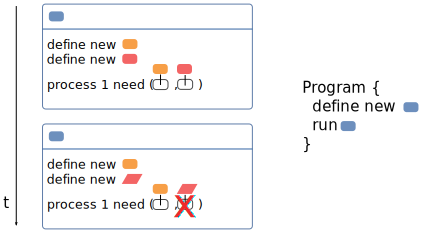
\includegraphics[width=.7\linewidth]{composants_principes_a.pdf}
  	}\qquad
  \subbottom[\label{subfig_decouplage:b}]{
	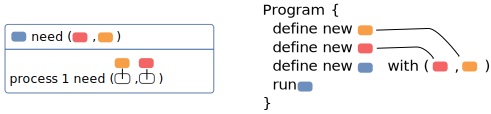
\includegraphics[width=.8\linewidth]{composants_principes_c.pdf}
  	}
  \subbottom[\label{subfig_decouplage:c}]{
	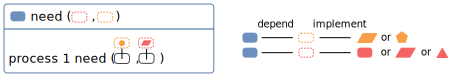
\includegraphics[width=.8\linewidth]{composants_principes_d.pdf}
  	}
 \end{sidecaption}
\end{figure}

Si l'on recontextualise ces principes dans le cadre de notre problématique, les classes de composants nécessaires à l'exécution minimale d'un algorithme évolutionnaire dans MGO sont décrites dans la figure \ref{fig:cake_classe}, et s'appuient sur le travail déjà décrit de la communauté des EA pour unifier la description de ces algorithmes.

\begin{figure}[!htbp]
	\begin{sidecaption}[Classe de composants nécessaires à l'exécution d'un algorithme évolutionnaire]{Classe de composants nécessaires pour l'exécution d'un EA.}[fig:cake_classe]
		\centering
		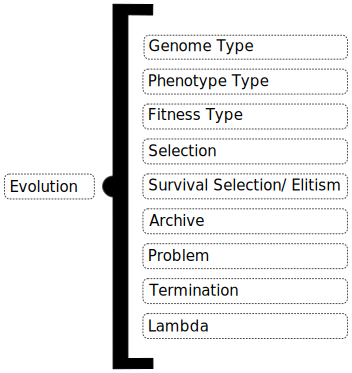
\includegraphics[width=0.7\linewidth]{cake_example.pdf}{
		}
  \end{sidecaption}
\end{figure}

Chacune de ces classes de composants est définie comme nécessaire pour le fonctionnement d'un algorithme d'évolution, dont la mise en dynamique du comportement générique est implémentée dans le composant \keyword{Evolution}. Tant que l'utilisateur n'aura pas fourni un composant compatible avec chacun de ces types de composants, alors le composant \keyword{Evolution} ne pourra pas s'exécuter. Le programme est défini comme un texte à trou, les boîtes sont bien placées, et le programme prêt à être exécuté suivant cet ordre, seulement ce n'est qu'un patron, une image, et cet ensemble de boîtes dont seule une partie de la logique a été intégrée, doit encore être complété par l'utilisateur. C'est un peu comme un puzzle dans lequel il manque des pièces, vous devez soit créer de nouvelles pièces, soit retrouver les pièces qui respectent la forme de chaque emplacement pour que le puzzle soit de nouveau complet.

L'inversion de contrôle détaillée dans les paragraphes précédents se matérialise de nouveau ici au travers du fait que c'est l'utilisateur qui définit sa composition, en s'assurant avec l'aide des instructions du programme que les dépendances propres au fonctionnement de chacun des composants sont bien fournies. Tout programme ne remplissant pas les conditions renverra un message d'erreur à son exécution. En ce sens MGO est probablement plus un \textit{\textit{framework}} qu'une librairie logicielle\Anote{martin_fowler}. L'autre avantage d'une telle approche c'est que l'application peut être livrée avec un vaste catalogue de pièces compatibles avec chaque type d'emplacement, laissant à l'utilisateur la possibilité de choisir sa propre combinaison, voire même de créer ses propres pièces s'il estime qu'elles sont manquantes.

Il existe différentes techniques pour qu'une telle architecture puisse être mise en oeuvre. Par exemple, l'utilisation mixte de \textit{classe abstraite} et d'\textit{interfaces} permettent dans de nombreux langages informatiques, comme Java ou C\#, de reproduire le découplage entre composants tel qu'on l'a vu dans la figure \ref{fig:decouplage_principe}.

En réalité, pour certains programmeurs \textcite{Odersky2005}\Anote{odersky_note_cake} ce type de techniques, dont l'existence, les avantages et les contraintes ont largement été discutés, ne constitue pas selon lui la meilleure réponse d'un point de vue technique pour garantir une meilleure réutilisabilité des composants informatiques. Il faut savoir à ce sujet qu'il existe en informatique une branche de recherche tournée vers la construction de langage de programmation aux caractéristiques innovantes. Ainsi les propriétés du langage Scala utilisé pour implémenter MGO exposent la solution fournie par Martin Odersky à cette problématique que représente la recherche d'une meilleure modularité des programmes informatiques. Tout comme dans les années 1980, le langage Smalltalk d'Alan Kay a introduit une autre façon de structurer les programmes avec le paradigme Orienté Objet, Scala permet ici de penser de façon originale la modularité des composants en usant d'un tout nouveau couplage de différentes abstractions informatiques ( \textit{abstract type members}, \textit{explicit self-types}, \textit{modular mixin composition})\Anote{note_informatique_mixin}. Autrement dit, ce que Scala va nous permettre d'exprimer comme degré de modularité lors de la description informatique de nos composants constitue en soi une innovation qui n'est pas présente, ou présente sous des formes trop complexes vis-à-vis de notre cahier des charges, dans bien d'autres langages informatiques.

%Si l'utilisation de classe abstraite est donc intéressante, elle ne résout pas tout les problèmes à elle seule. Ainsi par exemple, lorsqu'on utilise des classes abstraites, il n'est pas possible d'utiliser des dépendances cycliques entre composants, et la nécessité de respecter un ordre d'initialisation entre composants devient également rapidement une contrainte.

%Scala permet par exemple de définir des \keyword{traits} qui possède des caractéristiques plus intéressant que des classes abstraites ou des interfaces, tout en assurant à minima un comportement similaire. Il est par exemple possible d'assembler, de mixer de façon dynamique plusieurs traits, et l'addition des comportements se fait automatiquement.

%Il est également possible de définir des traits qui contiennent totalité ou seulement partie d'une implémentation. Ce type de programmation n'est pas permises par d'autres langage informatique, comme Java par exemple.

Souvent appelé de façon jargonnesque \foreignquote{english}{Cake Pattern} pour la possibilité de composition qu'elles offrent (comme dans un cake, un gâteau dont la recette peut accueillir une très grande variété d'étapes, de composantes), ces outils aussi connus sous le nom \foreignquote{english}{Scalable Component Abstractions} ou encore \foreignquote{english}{Component Based Dependency Injection} regroupent  l'ensemble des techniques permettant d'accéder à cette modularité qui est donc présente de façon native dans le langage, car pensée et implémentée par son créateur \autocite{Odersky2005}. La figure \ref{fig:principe_mixin} expose plus en détail ce principe, et les conséquences que cela peut avoir dans la construction d'un programme.


%Utilisé de façon complémentaire ces deux techniques permettent une grande flexibilité, une méthode ou un attribut est définit comme abstrait, et son implémentation doit être apportée par un composant externe.

%utilisant le cake pattern ( abstract type members, explicit self-types, modular mixin composition )
\cite{}
\begin{figure}[!p]
	\begin{sidecaption}[Illustrations des erreurs amenées par la découverte d'éléments manquants]{Un exemple plus proche de l'implémentation, appuyé par une version UML orientée Scala \autocite{Rachimow2009}, pour comprendre comment les élements manquants (attributs, méthodes) définis en \sqbox{tangoRed1} dans ce diagramme de classe sont indiqués au programme lors de la création de nouveaux objets. Les boîtes rouges représentent les erreurs retournées à l'utilisateur lors des tentatives successives de déclaration d'un nouvel élément \keywordmin{D1}, puis \keywordmin{D2}. \parbox{\marginparwidth}{
\begin{enumerate}[label=(\alph*),labelindent=\parindent,leftmargin=*]
       \item Un diagramme UML pour illustrer un scénario de dépendance entre trois composants exemples \keywordmin{A}, \keywordmin{B}, et \keywordmin{C}. Le composant A utilise une fonction run qui nécessite la définition d'une \keywordmin{methode\_b} et d'une \keywordmin{methode\_c} provenant d'un composant de type \keywordmin{B} et \keywordmin{C}.
       \item Un premier scénario illustre de façon simplifiée la logique d'héritage permettant la création d'un nouveau composant D1 à partir des composants A, B1 et C1.
       \item Dans ce deuxième scénario, on illustre la nécessité de redéfinir dans D2 les attributs, mais également les méthodes, qui n'ont pas été apportés par des composants extérieurs.
\end{enumerate}}}[fig:principe_mixin]
	\centering
	\subbottom[\label{subfig_principe_mixin_a}]{
		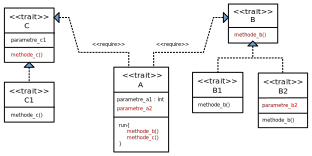
\includegraphics[width=0.8\linewidth]{exemple_mixin.pdf}
		}
	\subbottom[\label{subfig_principe_mixin_b}]{
		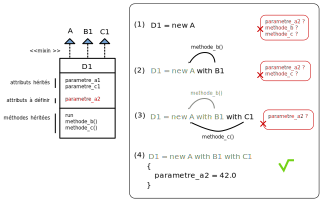
\includegraphics[width=0.8\linewidth]{exemple_mixin2.pdf}
		}
	\subbottom[\label{subfig_principe_mixin_c}]{
		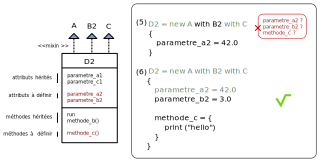
\includegraphics[width=0.8\linewidth]{exemple_mixin3.pdf}
		}
	\end{sidecaption}
\end{figure}

\pagebreak

\subsubsection{Mobiliser les bons composants}

Un des grands défauts de cette technique, c'est qu'elle rend souvent la lecture du code source plus difficile du point de vue d'un observateur extérieur. Le programme est en effet morcelé dans un ensemble de composants contenant chacun une petite partie de la logique du programme total, assemblé par le compilateur avant l'exécution du programme. De plus, lorsque l'utilisateur choisit un composant, celui-ci ne fait pas qu'offrir de nouvelles alternatives à l'utilisateur, il en retire également, comme on pourrait s'y attendre lorsqu'on manipule un arbre de dépendance complexe.

\begin{figure}[!htbp]
	\begin{sidecaption}[Scénario pour la sélection de composants]{Illustration d'un premier scénario dans la sélection de composant parmi les types $X$, et $Z$}[fig:composant_expli1]
		\centering
		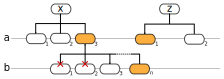
\includegraphics[width=0.7\linewidth]{dependanceExemple.pdf}{
		}
  \end{sidecaption}
\end{figure}

Si l'on considère un programme simplifié ayant besoin de deux types de composants pour fonctionner : $X$ et $Z$. Dans le premier scenario \ref{fig:composant_expli1}, l'utilisateur a choisi le composant $Z(a1)$ autonome, ainsi que le composant $X(a3)$. Ce dernier, contrairement au composant $X(a1)$ et $X(a2)$, dépend de nouveaux composant définis sur la ligne $b$ du schéma. On voit que dans les nombreux composants disponibles dans cette catégorie, seuls quelque-uns s'avérent compatibles avec le reste de la configuration de composants choisis par l'utilisateur. Que se passe-t-il lorsque l'utilisateur choisit pour $Z$ le deuxième composant $Z(2a)$ ?

\begin{figure}[!htbp]
	\begin{sidecaption}[Deuxième scénario pour la sélection de composant]{Illustration d'un deuxième scénario dans la sélection de composant parmi les types $X$, et $Z$.}[fig:composant_expli2]
		\centering
		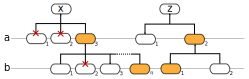
\includegraphics[width=0.7\linewidth]{dependanceExemple2.pdf}{
		}
  \end{sidecaption}
\end{figure}

C'est ce scénario qui est développé dans l'exemple \ref{fig:composant_expli2}. On voit que le choix de $Z(2a)$ implique de nouvelles restrictions de choix dans la branche $X$, mais aussi la possibilité de nouveaux choix. Ainsi $X(b1)$ qui n'était pas compatible avec le composant $Z(a1)$ dans le premier scénario, redevient ici compatible avec le composant $Z(b1)$ dont dépend $Z(a2)$ selectionné par l'utilisateur.

%Prenons un exemple simple, si l'utilisateur décide de ne pas utiliser de composant pour l'\keyword{Archive} des meilleurs individus, alors c'est tout un ensemble de stratégies dépendant de l'existence de ce composant dans le programme qui ne peux plus être mobilisé.

\subsubsection{Définition d'une méta-heuristique dans MGO}

L'implémentation d'un algorithme méta-heuristique prend cette forme dans MGO :

\begin{listing}[H]

\begin{minted}[linenos=true,frame=single,fontsize=\footnotesize]{scala}

trait NSGAII <: Evolution
  with BinaryTournamentSelection
  with TournamentOnRankAndDiversity
  with NonDominatedSorting
  with SBXCrossover
  with PolynomialGAMutation
  with GAGenome
  with Crowding
  with Pareto
  with NonStrictDominance
  with NoArchive
  with GeneticBreeding
  with MGFitness

\end{minted}
\caption{Exemple de définition d'une méta-heuristique dans MGO}
\label{alg:nsga2}
\end{listing}

La structure interne des composants constitutifs de l'algorithme NSGA2 est lisible dès lors qu'on a déjà étudié le fonctionnement de métaheuristique. Chacune des briques (ici une par ligne) peut être remplacée ou modifiée à partir du moment où les conditions de dépendance entre composants sont respectées (voir la figure \ref{fig:nsga_mgo} pour un exemple)

\begin{figure}[ht]
	\begin{sidecaption}[Représentation de NSGA2 dans MGO sous forme de composants]{Schéma de dépendance existant entre les différents types de composants pour la définition de l'algorithme NSGA2 sous MGO}[fig:nsga_mgo]
		\centering
		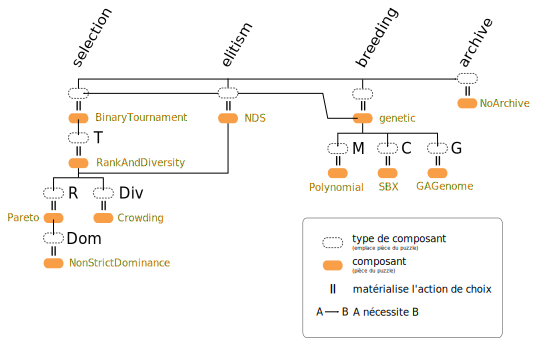
\includegraphics[width=0.9\linewidth]{diagrammeclassemgo.pdf}{
		}
  \end{sidecaption}
\end{figure}

Avoir accès de façon aussi lisible à la structure interne des algorithmes métaheuristiques permet de mieux comprendre ce qui les différencie. Prenons un exemple simple de construction d'algorithme génétique multi-objectif utilisant l'algorithme de classement de solution candidates dites du \textit{Non Dominated Sorting} (NDS), tiré de \autocite{Goldberg1989} et implémenté par Deb dans NSGA \autocite{Srinivas1994} puis NSGA2 \autocite{Deb2001}. Pour fonctionner dans ces deux variantes, \enquote{élitistes} ou \enquote{non élitistes}, ce composant NDS a besoin que l'utilisateur choisisse deux autres composants de type \keyword{Ranking}, et de type \keyword{Diversity}. Dans sa version non élitiste, le composant \keyword{Diversity} n'est pas utilisé.

Dans cette brique NDS, les individus $x$ de la population $p_1$ sont partitionnés selon un premier critère $c_1$, et de l'ensemble de partitions ainsi formées, on ne retient que la première pour former un front $f$. Les individus qui intègrent ce front sont supprimés de la population $p_1$, puis on recommence cette opération $n$ fois, cela jusqu'à ce que la somme des individus contenus dans l'ensemble des fronts $f_n$ soit égale à la population attendue à la fin de cette opération, c'est-à-dire $p_2$.

\begin{itemize}
\item Dans une utilisation non élitiste de cet algorithme, comme NSGA, la population au départ et la même qu'à la fin : $p_1 = p_2$. On a juste effectué un classement de cette population.
\item Dans une version élitiste, comme celle de NSGA2, la population $p_1$ est supérieur en taille à la population $p_2$. $p_1$ accueille ainsi la population $p_2$ précédemment évalué auquel on ajoute les résultats de sa progéniture (\textit{offspring}) évalué à $t + 1$. Comme tous les individus de $p_1$ ne pourront pas participer à $p_2$ car $p_2 = p_1 / 2$, l'inclusion du dernier front dans $p_2$ doit être géré comme un cas particulier (exemple, si le dernier front calculé dans $p_1$ contient $5$ individus, mais que la place disponible dans $p_2$ est de $3$ individus seulement) et $p_1$ doit être tronqué de façon intelligente, pour éviter de perdre en diversité de solution. On fait donc appel à une méthode supplémentaire de calcul de diversité qui constitue en soit un deuxième critère de selection $c_2$ discriminant les individus les uns par rapport aux autres.
\end{itemize}

Le choix d'un composant \keyword{Ranking} va déterminer quel va être le critère $c_1$ utilisé, et le choix d'un composant \keyword{Diversity} va déterminer selon quel critère $c_2$ les individus participant au dernier front vont être sélectionnés.

On voit bien que les stratégies permettant de fixer ces deux critères peuvent être de nature très différentes. Pour $c_1$ le critère le plus classique est le critère de dominance de Pareto défini par le composant du même nom \keyword{ParetoRanking}, mais d'autres critères sont tout à fait envisageables.

Inversement, la même brique atomique \keyword{ParetoRanking} définissant le calcul de dominance de Pareto est ainsi utilisée pour différents algorithmes canoniques, comme MOGA ou bien NSGA2. Seulement là ou NSGA2 va faire appel à cette brique plusieurs fois dans le composant NDS (le calcul de dominance est réalisé à chaque retrait d'individus de la population $p_1$ afin de recalculer les nouveaux individus non dominés), MOGA va utiliser ce composant une seule fois en l'encapsulant dans un autre composant qui implémente la façon dont MOGA partitionne les individus. On peut voir le détail de ces calculs et leur impact sur la valeur de \textit{fitness} associée à chaque individu dans le tableau \ref{pranking:b} déjà présenté.

Pour $c_2$, le critère utilisé par NSGA2 est une distance de \textit{crowding}, mais là aussi d'autres variantes existent, comme par exemple le calcul d'Hypervolume \autocite{Fonseca2006}. Cette brique \keyword{HypervolumeMetric} est aussi implémentée dans MGO, et participe à différentes étapes dans l'algorithme métaheuristique SMS-EMOA de \textcite{Emmerich2005}.

Le défaut majeur d'une telle approche, c'est qu'elle ne renseigne pas immédiatemment l'expérimentateur sur les choix valides ou invalides qui sont à sa disposition, et celui-ci peut alors se perdre dans une logique d'exécution du code très éclaté. Pour résoudre ce problème, deux stratégies sont mises en oeuvre, la première c'est celle que l'on observe dans le listing \ref{alg:nsga2}, à savoir l'implémentation pré-existante dans le \textit{framework} de plusieurs algorithmes évolutionnaires canoniques prêt à l'emploi, et donc également prêt à être modifiés, comme CMAES \autocite{Hansen2001}, NSGA2 \autocite{Deb2001}, ou SMS-EMOA \autocite{Emmerich2005}. La deuxième stratégie repose sur un outil en cours de développement par Mathieu Leclaire. Nommée \textit{JANET}, cette application est capable de lire et de reconstruire le graphe de dépendance entre les différents composants d'un programme qu'on lui donne à explorer. A partir de là, il autorise l'expérimentateur à composer son propre graphe de façon totalement interactive, en cliquant sur les composants du graphe.

A chaque sélection de composant dans le graphe, l'ensemble des dépendances est recalculé afin de montrer à l'utilisateur quelles dépendances sont accessibles et valides/invalides à partir de son choix. Enfin \textit{JANET} est capable de générer un squelette de code à partir de la sélection réalisée par l'utilisateur, similaire à celui exprimé dans le listing \ref{alg:nsga2}, utilisable directement comme nouvel algorithme.

\subsubsection{Définition d'un problème d'optimisation}

La librairie est conçue de façon à être totalement indépendante, car elle intègre à la fois les concepts nécessaires à la définition, et la résolution de problèmes d'optimisations. En ce sens, elle peut être utilisée ou intégrée à n'importe quel autre logiciel qui respecte le formalisme mis en place.

Le listing \ref{alg:Schaffer} est un exemple de définition d'un problème d'optimisation dans MGO. Dans celui-ci, il s'agit de résoudre la fonction test F2 multi-objectif de Schaffer \textcite[94]{Schaffer1985}, déjà définie dans l'équation \ref{eq:schaffer}.

\begin{listing}[!htbp]

\begin{minted}[linenos=true,frame=single,fontsize=\footnotesize]{scala}

trait Schaffer extends GAProblem with MGFitness {

  def genomeSize = 1
  def min = Seq.fill(genomeSize)(-100000.0)
  def max = Seq.fill(genomeSize)(100000.0)

  type P = Seq[Double]

  override def express(g: Seq[Double], rng: Random) = Seq(f1(g(0)), f2(g(0)))
  override def evaluate(p: P, rng: Random) = p

  def f1(x: Double) = pow(x, 2)
  def f2(x: Double) = pow(x - 2, 2)

}

\end{minted}
\caption{Exemple de définition d'un problème multi-objectifs dans MGO}
\label{alg:Schaffer}
\end{listing}

La ligne 5 contient la signature du composant, et indique à MGO qu'il s'agit d'un problème de type algorithmes génétiques \keyword{GAProblem} de type multi-objectif \keyword{MGFitness}.

Pour que le composant \keyword{GAProblem} soit opérationnel, celui-ci a besoin que l'utilisateur lui fournisse un certain nombre d'éléments en entrée : une taille de génome \keyword{genomeSize}, un type de Phenotype \keyword{P}, la définition des fonctions \keyword{express(...)} et \keyword{evaluate(...)}.

\begin{figure}[ht]
	\begin{sidecaption}[Hiérarchie entre les composants pour la fonction test F2 de Schaffer]{Hiérarchie entre les composants pour la définition d'un problème, un exemple avec la fonction de test F2 de Schaffer}[fig:hierarchieComposants]
	 \centering
	 	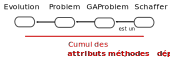
\includegraphics[width=.5\linewidth]{HierarchieComposants.pdf}
	\end{sidecaption}
\end{figure}

Si l'on regarde les dépendances de \keyword{GAProblem}, alors on voit qu'il dépend de \keyword{Problem}, lui-même étant défini comme étant une extension d'\keyword{Evolution}. Concrétement, cela veut dire que le problème Schaffer ne pourra être résolu que si l'ensemble des composantes cumulées de \keyword{GAProblem} , \keyword{Problem} et \keyword{Evolution} sont satisfaites au moment de la résolution du programme par le compilateur, défini dans la section ci-dessous.

Les fonctions $f1$ et $f2$ prennent un seul et même paramètre de variation $x$ non contraint. La taille \keyword{genomeSize} du génome est donc fixée à $1$, et la définition des variables \keyword{min} et \keyword{max} permet d'associer à $x$ un intervalle de variation autorisé compris entre $[-10^{5}$, $10^{5}]$.

Le type \emph{P} indique la nature du phénotype attendu pour ce problème. Dans notre cas, la représentation d'une solution candidate dans l'espace de solution $\mathbb{X}$ correspond à un vecteur de réels \emph{Seq[Double]} qui accueille le résultat des fonctions objectifs $f1$ et $f2$.

Les deux fonctions \keyword{express(...)} et \keyword{evaluate(...)} doivent également être définies car elles sont utilisées par le composant \keyword{Evolution}, et fixent les règles de constitution d'un \keyword{Individu}, une structure de données permettant de regrouper le génome, le résultat des fonctions objectifs pour ce génome, ainsi que le résultat de la future \textit{fitness}.

\begin{itemize}[label=\textbullet, noitemsep, topsep=0pt, parsep=0pt, partopsep=0pt]
\litem{\keyword{express()}} prend en paramètre un vecteur de double qui correspond à la taille du génome. Dans le cas de Schaffer, il n'y a qu'un seul paramètre $x$, donc le génome $g$ est de taille 1, et donc $g(0)$ correspond forcément à la seule valeur $x$ contenue dans le génome. Cette fonction retourne l'\enquote{expression de la fonction objective à évaluer}, donc un vecteur contenant l'expression (ou la définition) des deux fonctions objectives $f1$ et $f2$ à évaluer. Cette fonction n'évalue pas, mais définit quelle est la marche à suivre pour évaluer.

\litem{\keyword{evaluate()}} est une fonction qui prend un phénotype en entrée et renvoie en sortie un vecteur de valeur correspondant à l'évaluation des fonctions objectifs. Ici les valeurs de $f1$ et $f2$.

\end{itemize}

Dans le cas d'une simulation, \keyword{express()} est la fonction qui va \textbf{exécuter le modèle de simulation} et récupérer les valeurs résultats en sortie, qui constitue le Phénotype. Dans ce cas-là, le phénotype ne permet pas forcément de discriminer les résultats de deux simulations. Ces sorties peuvent donc prendre la forme d'indicateurs directement utilisables comme fonction objectifs, mais elles peuvent également n'être que des données brutes dont il faut encore faire l'analyse pour dériver des fonctions objectifs. La fonction \keyword{evaluate()} \textbf{renvoie le vecteur résultat des fonctions objectifs après application sur les sorties de simulation}. Un \keyword{Individu} dans la \keyword{Population} est une structure de données composée d'un Genome (paramètres du modèle de simulation), du résultat de la fonction \keyword{express} qui transforme un Génome en Phénotype (exécution de la simulation et récupération des résultats), et du résultat de la fonction \keyword{evaluate} qui transforme un Phenotype en vecteur de valeurs d'objectifs.

%difference par rapport aux autres librairies ?

\paragraph{Exécution d'un problème d'optimisation avec MGO}

\begin{listing}[H]

\begin{minted}[linenos=true,frame=single,fontsize=\footnotesize]{scala}

object TestNSGAII extends App {

  val resolve =
    new Schaffer with NSGAII with CounterTermination {
      def steps = 1000
      def mu = 200
      def lambda = 200
      def genomeSize = 1
    }

  implicit val rng = newRNG(42)

  val res =
    resolve.evolve.untilConverged {
      s => println(s.generation)
    }
}

\end{minted}
\caption{Evaluation d'un problème multi-objectifs à l'aide de l'algorithme NSGA2}
\label{alg:Evaluation_Schaffer}
\end{listing}

Dans l'implémentation \ref{alg:Evaluation_Schaffer}, la variable \keyword{resolve} contient la définition de la marche à suivre : il s'agit ici de résoudre le problème \keyword{Schaffer} (voir \ref{alg:Schaffer}) en utilisant la métaheuristique \keyword{NSGA2} (voir \ref{alg:nsga2}) en utilisant un indicateur de fin d'optimisation de type compteur de générations \keyword{CounterTermination}.

Les variables \keyword{steps} (nombre d'itérations avant arrêt de la métaheuristique), \keyword{mu} (taille de la population), \keyword{lambda} (taille de la progéniture), \keyword{genomeSize} (taille du génome) sont des variables qui n'ont pas trouvé de valeurs dans la résolution du graphe de dépendance reliant les différents composants.

En cas de non-définition de ces quatre variables (ce qui n'est pas le cas ici, comme on le voit dans \keyword{resolve}), le compilateur fera remonter sous forme d'erreurs à la compilation la nécessité pour l'utilisateur de définir ces variables.

\subsubsection{La mise en oeuvre du couplage MGO - OpenMOLE }

Dans la section justifiant la création d'un nouveau \textit{framework} dédié aux méta-heuristiques, on a abordé des points d'objectifs à la fois centrés sur les capacités finales de MGO en tant que \textit{framework} flexible, extensible, autonome; mais également sur les autres capacités attendues pour une utilisation de ce \textit{framework} dans un outil spécialisé dans la distribution transparente des calculs sur environnement HPC, à savoir OpenMOLE.

Concevoir des logiciels capables de s'exécuter sur des environnement distribués est une spécialité informatique en tant que telle, usant de technologies et de jargon déjà difficiles d'accès à des développeurs spécialisés, et donc encore moins accessibles à un public plus interdisciplinaire comme les chercheurs en SHS.

Il n'est donc pas question d'associer, du moins dans un premier temps, une myriade d'interfaces au \textit{framework} MGO à destination d'un couplage direct avec les technologies \textit{HPC} ou de \textit{Grid Computing}. Il me semble être beaucoup plus intéressant de ne pas complexifier outre mesure la librairie MGO, et de profiter du fait qu'il s'agit d'un \textit{\textit{framework}} pour composer des métaheuristiques plus adaptées à l'usage maximum qui peut être fait des ressources disponibles. En soit, MGO peut dans sa version autonome satisfaire un public scientifique exigeant sur le volet d'une recherche théorique dans le domaine des méta-heuristiques, tout en proposant dans un plugin pour OpenMOLE, des métaheuristiques adaptées à un tout autre public. Les modélisateurs sont attirés par l'efficience de ces algorithmes et leurs utilisations dans des cas d'utilisations spécifiques, souvent très différents des \textit{benchmarks} que l'on trouve par exemple dans la littérature des EA. Dans cette configuration, composer ses propres métaheuristiques reste toujours possible, mais demande un peu plus de connaissance technique pour modifier le code du plugin faisant l'interface entre MGO et openMOLE. Le tableau \ref{tab:resume_public_cible} aborde de façon synthétique ces deux points de vue utilisateurs par rapport aux principales qualités attendues du programme : Flexibilité, Extensibilité, Utilisabilité.

% http://www.tablesgenerator.com/latex_tables#
% Ajouter une couleur sur la partie +++ a mettre en valeur coté plugin MGO

\begin{table}[!htbp]
\begin{sidecaption}[Résumé des avantages et inconvénients à atteindre selon le public cible pour MGO]{Résumé des avantages et des inconvénients à atteindre selon le public cible. \parbox{\marginparwidth}{
\begin{enumerate}[label={},noitemsep,  parsep=0pt, partopsep=0pt, labelindent=0pt,leftmargin=*]
		\item $-$ assez difficile
		\item $-{}-$ difficile
		\item $-{}-{}-$ très difficile
		\item $+$ assez facile
		\item $++$ facile
		\item $+++$ très facile
\end{enumerate}}}
	[tab:resume_public_cible]
	\centering
	\begin{tabular}{llllll}
		\toprule
		\multicolumn{2}{l}{\multirow{2}{*}{}} & \multicolumn{2}{l}{modélisateur} & \multicolumn{2}{l}{informaticien} \\ \cline{3-6}
		\multicolumn{2}{l}{} & Plugin Mgo & Mgo & Plugin Mgo & Mgo \\
		\midrule
		(1) & Flexible & $-{}-$ & $+$ & $+$ & $+++$ \\
		(2) & Extensible & $-{}-{}-$ & $-$ & $+$ & $++$ \\
		(3) & Utilisable & $+++$ & $+$ & $+++$ & $+++$ \\
		\bottomrule
		\end{tabular}
  \end{sidecaption}
\end{table}

\begin{enumerate}[label=(\arabic*)]
\item du point de vue de la flexibilité des métaheuristiques proposées, c'est-à-dire de la possibilité de combinaisons de composants offertes par MGO, celle-ci doit être identique avec le plugin OpenMOLE ou directement dans MGO. Pour des non informaticiens, cette flexibilité reste beaucoup plus difficile à mettre en oeuvre avec le plugin OpenMOLE, car la logique d'exécution des métaheuristiques est \enquote{éclatée} dans différentes tâches d'un \textit{workflow} OpenMOLE afin que certaines d'entre elles soient parallélisées (voir la section suivante \ref{p:prototype_fonctionel}). De nouveaux algorithmes métaheuristiques plus spécialisés pour une utilisation sur grille de calcul font également leur apparition dans le plugin, et constituent des \textit{worflows} beaucoup plus complexes, assez difficilement accessibles à la modification par des modélisateurs géographes.

\item ajouter ou modifier de nouveaux algorithmes dans le plugin OpenMOLE nécessite de maîtriser suffisamment bien à la fois l'ensemble du vocabulaire (aussi appellé \textit{Domain Specific Language} DSL OpenMOLE) nécessaire pour définir des \textit{workflows}, mais également le langage de programmation Scala qui le supporte. Une fois ces premières connaissances acquises, et avant même de pouvoir créer de nouvelles métaheuristiques, il faudra comprendre en observant les métaheuristiques déjà implémentées comment d'une part, les composants MGO sont encapsulés et chaînés dans un \textit{workflow} complexe mêlant Scala et DSL OpenMOLE, et d'autre part, comment ce \textit{workflow} définissant l'algorithme peut être encapsulé dans une nouvelle primitive accessible directement au niveau du DSL (une forme \textit{workflow} paramétrable permis par les \textit{PuzzleWorkflows}). Si ce travail peut effectivement être réalisé sans trop de difficulté par un informaticien un peu expérimenté, l'exercice paraîtra très difficile voire hors de portée à un modélisateur géographe.

\item l'utilisation du plugin dans OpenMOLE doit être rendue la plus simple possible pour le modélisateur et l'informaticien. En revanche l'utilisation du \textit{framework} de façon autonome demande pour un modélisateur quelques compétences techniques supplémentaires pour installer les logiciels adéquats permettant de modifier et compiler MGO. Une fois cette barrière technique dépassée, la connaissance du langage Java ou Scala est certes nécessaire pour modifier ou ajouter des composants, mais elle ne l'est pas forcément lorsqu'il s'agit d'imbriquer et de paramétrer les composants correctement.

\end{enumerate}

Si le \textit{framework} MGO est parfaitement utilisable de façon autonome, celui-ci ne bénéficie pas dans ce mode d'utilisation des algorithmes dédiés pour une utilisation sur des environnements distribués. Or, c'est bien ce cas d'utilisation que nous voulons rendre disponible aux modélisateurs, à la différence des librairies intégrées existantes, par exemple dans le \textit{behaviorSearch} de Netlogo \autocite{Stonedahl2011a}.

La mise à disposition de ce \textit{framework} dans le cadre d'un plugin pour OpenMOLE fait intervenir de tous nouveaux objectifs, cette fois-ci relatifs aux intérêts des modélisateurs. En effet, si les métaheuristiques se doivent effectivement d'être modifiables, ce n'est pas forcément cet aspect qui prime pour une utilisation dans la modélisation; qui appelle une fois la base du modèle réalisé, des cycles de développements assez courts, ceux-ci se limitant la plupart du temps à des ajouts, des modifications, ou des retraits d'hypothèses. L'utilisation de métaheuristiques, même canoniques, est un premier palier d'utilisation utile pour tenter de discriminer au plus vite les modèles de simulation. Dans ce cas, c'est bien les propriétés d'efficacité et d'indépendance au problème que l'on mobilise dans l'utilisation de métaheuristique.

La modification de la structure interne d'une métaheuristique est un cas d'utilisation qui vise l'adaptation plus précise et ciblée de la réponse d'une métaheuristique pour un problème donné. Il en résulte une perte de généralité nécessaire.

\subsection{Premier prototype fonctionnel}
\label{p:prototype_fonctionel}

La constitution d'un premier prototype fonctionnel constitue pour l'équipe un triple retour d'expérience, pour MGO, pour OpenMOLE, et évidemment pour le modèle utilisé, à savoir SimpopLocal.

Avant mars 2012, le couplage entre MGO et OpenMOLE est réalisé par l'utilisateur lors de la définition des \textit{workflows}. Grâce à la nature autonome et modulaire des composantes fournis par l'univers du \textit{framework} MGO, la logique d'exécution d'une métaheuristique peut facilement être retranscrite dans le référentiel d'OpenMOLE. Les tâches d'un \textit{workflow} vont tout simplement encapsuler les appels et les objets spécifiques aux différentes composantes de la métaheuristique, en apportant la logique nécessaire à une exécution de certaines de ces composantes dans un environnement de calcul distribué.

Autrement dit, la logique d'exécution générique d'une métaheuristique décrite dans la composante \keyword{Evolution} est d'abord instanciée (par exemple on choisit d'utiliser les composants de NSGA2) puis éclatée dans un ensemble de tâches dont l'organisation est guidée à la fois par la reproduction de cette optimisation, mais aussi par la parallélisation de certaines de ces tâches.

Un tel \textit{workflow} doit également s'acclimater de toute la logique d'expérimentation pour un modèle de simulation. Des tâches intermédiaires font donc leur apparition dans le \textit{workflow} pour gérer ce tout nouveau plan d'expérience particulier.

La nature intrinsèquement parallèle des algorithmes évolutionnaires tient dans la possibilité d'évaluer non pas les solutions candidates une par une, mais bien d'un seul coup, par l'évaluation de l'ensemble des solutions candidates d'une population à un instant $t$. La première étape a donc été de distribuer l'évaluation des solutions candidates sur un environnement distribué, afin de bénéficier d'une exécution quasi-simultanée de l'ensemble des solutions candidates de la population.

\begin{figure}[H]
	\begin{sidecaption}[Le premier workflow prototype pour utiliser des algorithmes évolutionnaire avec MGO dans OpenMOLE]{La tâche d'exploration est en bleu \sqbox{tangoBlue1}, celle d'agrégation en rouge \sqbox{tangoRed1}}[fig:openmole_wf]
		\centering
		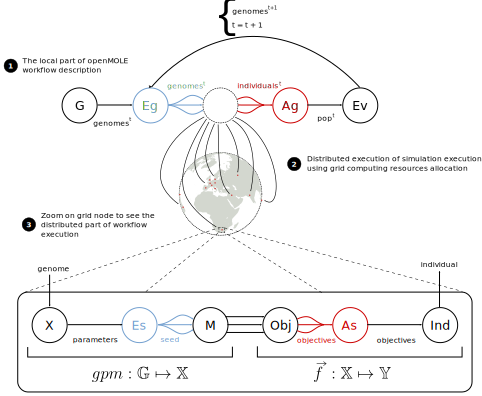
\includegraphics[width=1.1\linewidth]{wf_openmole_mgo_1.pdf}{
		}
  \end{sidecaption}
\end{figure}

On considère les paramètres suivants, une population initiale de génomes $n$, et le nombre de réplications à exécuter pour chacun de ces génomes équivalent à $r$; Autrement dit, à chaque itération $t$ de l'algorithme d'optimisation, c'est $n$ jeu de valeurs de paramètres différents ($= n$ génomes) qui vont chacun être testés $r$ fois avec des graines aléatoires différentes. Soit un total final de $n * r * t$ simulations.

Avant de rentrer dans les détails du \textit{workflow}, il est également important de rappeller que dans celui-ci, un \keyword{Genome}, et par la suite un \keyword{Individu} dans une \keyword{Population}, sont deux dénominations qui désignent avant tout un jeu de valeurs de paramètres, même si un individu représente on va le voir un peu plus que çà. Autrement dit, quand on discute ici de la qualité d'un \keyword{Individu} et de son positionnement dans l'espace des objectifs $\mathbb{Y}$, c'est sous-entendu en référence au jeu de valeurs de paramètres qui a permis d'obtenir ce même \keyword{Individu}.

Le premier niveau de \textit{workflow} (étape \circled{1} dans la figure \ref{fig:openmole_wf}) opérant de façon locale sur la machine ou le serveur de l'utilisateur est décrit ainsi :

%\begin{itemize}[label=\textbullet]

\begin{myitemize}

\item[G] Cette tâche définit comment le problème va être représenté par le \keyword{Genome} durant l'optimisation. C'est aussi à ce moment là que le mapping est réalisé avec les paramètres du modèles, avec par défaut 1 gène par paramètre $p$ du modèle. Cette tâche génère ensuite un ensemble de génomes $g_i \in \{g\}, i \in \{1 \dotsc n\}$ chacun étant initialisé par des valeurs de paramètres aléatoires.

\item[Eg] Cette première tâche d'exploration exécute un plan d'expérience qui associe à chaque \keyword{Genome} $g_i$ une liste de graines aléatoires  - ou \textit{seeds} - $\{s_i\}$. Cette liste d'éléments $s_{i,r} , s_{i,r} \in \{s_i\}, r \in \{1 \dotsc r\}$ est de taille égale au nombre de réplications $r$ définies en paramètre de l'expérimentation. De ce plan d'expérience résulte la création d'un ensemble $\{w\}$ de sous \textit{workflows} équivalent au nombre de génomes initial $n$. Chaque $w_i$ est organisé selon la description du deuxième niveau de \textit{workflow} décrit ci-dessous, distribué de façon transparente sur un des noeud de la grille de calcul par OpenMOLE (étape \circled{2} dans la figure \ref{fig:openmole_wf}) avec pour paramètre d'entrée le vecteur $(g_i, \{s_i\})$.

\item[Ag] Chaque sous \textit{workflow} $w_i$ s'executant sur grille renvoie un \keyword{Individu} évalué, une structure de donnée qui associe pour chaque \keyword{Genome} $g_i$, un \keyword{Phenotype} et un vecteur d'objectifs $f_i$. Cette tâche d'aggrégation collecte ces individus auprès de l'ensemble des sous \textit{workflow} de façon à former un ensemble d'\keyword{Individu} formant une nouvelle \keyword{Population} $P$. Cette dernière est ensuite transmise pour examen à la tâche suivante \textit{Ev}.

\item[Ev] Cette tâche contient le coeur de l'algorithme d'optimisation, dont le comportement est fonction de l'algorithme évolutionnaire selectionné ou composé, et des paramètres choisi par l'utilisateur pour celui-ci. Dans une première phase, la population nouvellement constituée est fusionnée avec la population d'individu de la génération précédente. Une fitness est attribuée à chaque individu de cette nouvelle population, ce qui permet de caractériser la qualité de chacune de ces solutions dans l'espace des objectifs de façon relative à l'algorithme utilisé. S'ensuit alors une première phase élitiste de selection qui opère sur la base de ce score. Les individus selectionnés participent ensuite de nouveau à un tirage au sort pour tenter d'intégrer le pool d'individu (\textit{mating pool}) participant à la reproduction, étape durant laquelle emerge un ensemble de nouveaux génomes à évaluer, transmis à la tâche \textit{Ev} pour une nouvelle distribution.
\end{myitemize}

Le deuxième niveau de workflow (étape \circled{3} dans la figure \ref{fig:openmole_wf}), celui qui s'exécute sur un noeud distant de la grille de calcul, contient les tâches suivantes :

\begin{myitemize}

\item[X] Cette tâche extrait les valeurs de paramètre du génome $g_i$ qui est donné en entrée de ce sous workflow, et les transmets avec l'ensemble des $r$différentes \textit{seeds} de l'ensemble $\{s_i\}$ à une nouvelle tâche d'exploration \textit{Es}

\item[Es] définit un nouveau plan d'expérience pour exécuter l'ensemble des réplications $s_{i,r}$ sur ce noeud local de la grille. A chaque réplication du modèle de simulation est associé un jeu de valeur de paramètre tel qu'il a été extrait du génome $g_i$ (toujours identique donc), ainsi qu'une \textit{seed}, prise dans $s_{i,r}$ avec $r$ différent pour chaque réplication.

\item[M] exécute le modèle de simulation avec la graine aléatoire $s_{i,r}$ et le jeu de valeur de paramètre fourni. Cette étape est équivalente à la constitution du Phénotype.

\item[Obj] applique aux résultats de la simulation les fonctions objectifs définis par l'utilisateur dans le \textit{workflow}

\item[As] récupère les vecteurs de valeurs objectifs associées à chaque réplication du modèle de simulation, et les agrège selon une fonction statistique choisie par l'utilisateur, une moyenne ou une médiane par exemple.

\item[Ind] crée un \keyword{Individu}, une structure de donnée associant le \keyword{Genome} $g_i$ évalué et les valeurs d'objectifs. La \textit{seed} n'est pas conservé dans cette expérience ou on recherche avant tout un comportement robuste à l'aléa.

\end{myitemize}


Les premières explorations du modèle SimpopLocal ont été faites suivant ce \textit{workflow} à partir d'avril 2011, mais c'est seulement en septembre 2011 que le couplage est présenté aux géographes à l'ECQTG d'Athènes, puis à des informaticiens à la conférence V2CS à Paris.

Les premiers \textit{workflows}\Anote{cas_utilisation_wfom}, assez complexes et uniquement accessibles au format \enquote{scripts}, ont rapidement constitués des fichiers de plusieurs centaines de lignes (voir le site compagnon de la thèse). Cette évolution dans la taille des \textit{workflows} est rapidement devenue problématique à la fois pour la maintenance mais également pour la lisibilité de telles expérimentations. Un obstacle vis-à-vis de notre principal objectif, mettre à disposition des modélisateurs un outil dont le premier avantage est sa facilité de mise en oeuvre et sa réutilisabilité.

En mars 2012, Romain Reuillon décide d'intégrer ce \textit{workflow} présenté dans la figure \ref{fig:openmole_wf} directement dans OpenMOLE sous la forme d'un \textit{workflow} paramétrable (concept de \textit{Puzzle Workflow}). Il devient alors très facile de déclarer une exploration utilisant des Algorithmes Evolutionnaires au format scripts, quelques lignes suffisent, comme le montre l'encadré sur Ants. L'avantage d'une telle solution c'est qu'elle permet d'encapsuler cette complexité dans un workflow \enquote{prêt à lancer} tout en laissant la possibilité aux utilisateurs plus avancés de continuer à créer leurs propres workflows d'Algorithmes Evolutionnaire s'ils le souhaitent.

Si l'exécution d'un tel \textit{workflow} est déjà un premier pas vers une systématisation dans l'application de ces techniques d'optimisation à l'exploration des modèles de simulations, il faut soulever un autre point important aux yeux de l'utilisateur. Quelle performance peut-on en effet attendre d'un tel \textit{workflow} d'optimisation distribué lorsqu'il est appliqué sur un modèle de simulation relativement rapide en Netlogo ?

Si $n=200$, $r = 30$, $t=2000$, cela équivaut donc à $12$ millions de simulations. Pour nous donner une durée, il faut encore multiplier par la durée d'exécution du modèle : un modèle jugé relativement rapide s'exécutant en moyenne en $2$ minutes sous Netlogo revient à cumuler environ $46$ années de calcul sur un seul processeur. Sur une grille de calcul disposant de $1000$ processeurs, cette durée descend à $17$ jours. Sachant que de tels Algorithmes Evolutionnaires ne garantissent pas d'optimum global, ceux-ci doivent également être répliqués afin de vérifier si l'algorithme, ne serait pas malheureusement tombé dans un optimum local.

Il y a deux possibilités pour gagner en temps de calcul et permettre un retour d'expérience plus rapide sur les modèles pour les modélisateurs. En effet, soit le modèle de simulation peut être optimisé ou réécrit, soit l'algorithme métaheuristique distribuant les simulations peut encore être amélioré. Seule la deuxième voie offre un gain de temps générique, quel que soit le modèle. C'est pourquoi Romain Reuillon développe dès le mois d'Août 2012 une version des algorithmes évolutionnaire en îlots \autocite{Whitley1997}. L'idée est relativement simple (il existe plusieurs versions, on développe seulement la plus simple ici), au lieu d'avoir une seule population centrale, on propose d'avoir une population par noeud exploitée sur l'environnement distribué. Chacune de ces populations fonctionne de façon autonome sur le noeud, en exploitant les ressources disponibles sur celui-ci (les simulations sont lancées en parallèle si le noeud dispose de plusieurs processeurs/coeurs), et s'exécute ainsi jusqu'à ce que la condition d'arrêt soit remplie (durée, nombre de génération, convergence, etc.). Dès que l'un de ces noeuds termine, les meilleures solutions de cette population sont immédiatement rapatriées, puis comparées et hybridées avec une population centralisée sur l'ordinateur ou le serveur qui exécute le \textit{workflow}. Une nouvelle population de génome (valeurs de paramètres) est générée à partir de la population centrale, puis celle-ci est envoyée pour exécution autonome sur un noeud disponible dans l'environnement distribué. Avec cette stratégie, il n'y a plus aucun temps de latence dans le déroulement du \textit{workflow}, et le parallélisme des Algorithmes Evolutionnaires est exploité de façon maximale sur chaque noeud.

Dans le cas de SimpopLocal, la première voie a également été explorée, et le modèle écrit initialement en Netlogo, a d'abord accueilli un plugin en Scala pour externaliser les traitements les plus longs, avant d'être finalement réécrit complétement en Scala. Les Algorithmes Evolutionnaires en îlots ont également été utilisés pour l'exploration de SimpopLocal. On trouvera le \textit{workflow} correspondant à la publication \autocite{Schmitt2015} sur le ( \href{http://iscpif.github.io/ simpoplocal-epb/}{@site}.
